\documentclass[11pt]{article}
\usepackage[T1]{fontenc}
\usepackage[utf8]{inputenc}
\usepackage{geometry}
%\geometry{letterpaper,landscape}
\geometry{paperwidth=9in,paperheight=7in}
%\usepackage{hyperref}
\usepackage[pdftex,
            pdfauthor={Bruno Ruviaro},
            pdftitle={Uma Gentil Introdução ao SuperCollider},
            pdfsubject={tutorial de SuperCollider},
            pdfkeywords={computação musical, SuperCollider, programação, música},
            pdfproducer={LaTeX},
            pdfcreator={pdflatex}]{hyperref}
            
\usepackage{enumerate}
\usepackage{graphicx}
\usepackage{endnotes}
\usepackage{listings}

\usepackage{listings}
\lstset{%
        inputencoding=utf8,
        extendedchars=true,
        literate=%
        {é}{{\'{e}}}1
        {è}{{\`{e}}}1
        {ê}{{\^{e}}}1
        {ë}{{\¨{e}}}1
        {É}{{\'{E}}}1
        {Ê}{{\^{E}}}1
        {û}{{\^{u}}}1
        {ú}{{\'{u}}}1
        {â}{{\^{a}}}1
        {à}{{\`{a}}}1
        {á}{{\'{a}}}1
        {ã}{{\~{a}}}1
        {Á}{{\'{A}}}1
        {Â}{{\^{A}}}1
        {Ã}{{\~{A}}}1
        {ç}{{\c{c}}}1
        {Ç}{{\c{C}}}1
        {õ}{{\~{o}}}1
        {ó}{{\'{o}}}1
        {ô}{{\^{o}}}1
        {Õ}{{\~{O}}}1
        {Ó}{{\'{O}}}1
        {Ô}{{\^{O}}}1
        {î}{{\^{i}}}1
        {Î}{{\^{I}}}1
        {í}{{\'{i}}}1
        {Í}{{\~{Í}}}1
}

\usepackage[symbol*, perpage]{footmisc}
\usepackage[colorinlistoftodos]{todonotes}
\usepackage[framed, numbered]{sclang-prettifier}
\renewcommand{\lstlistingname}{Example}
\title{\textbf{A Gentle Introduction to SuperCollider}}
\author{Bruno Ruviaro}
\usepackage[yyyymmdd]{datetime}
\renewcommand{\dateseparator}{-}
\date{\today}
%\DeclareUnicodeCharacter{0177}{\^y}
\usepackage[brazilian]{babel}

\begin{document}

% This is the first page, just title, no page number
\topskip0pt
\vspace*{\fill}
\begin{center}
{\LARGE \textbf{Uma Gentil Introdução ao SuperCollider}}

\bigskip
por Bruno Ruviaro

\medskip
revisão \today

tradução: Rodolfo Valente e Bruno Ruviaro


\bigskip
\bigskip

\begin{figure}[h]
\begin{center}

\includegraphics[scale=1]{fig-by-sa.png}
\end{center}
\end{figure}

\bigskip
Esta obra é disponibilizada sob a licença Creative Commons

Attribution-ShareAlike 4.0 International License.

Para ler uma cópia desta licença, visite:

\url{http://creativecommons.org/licenses/by-sa/4.0/}.



\end{center}
\vspace*{\fill}
\thispagestyle{empty}
\clearpage

% This is the table of contents
\pagenumbering{roman}
\tableofcontents
\maketitle
\pagenumbering{arabic}

\renewcommand{\partname}{Parte}
\renewcommand{\figurename}{Figura}
\renewcommand{\notesname}{Notas}

% This is the body of the text
% Page numbers are reset to arabic

% PART I
\part{O BÁSICO}

\section{Olá mundo}

Pronto para criar seu primeiro programa em SuperCollider? Assumindo que você tem um SC aberto e funcionando à sua frente, abra um novo documento (menu File$\rightarrow$New ("Arquivo$\rightarrow$Novo") ou o atalho [ctrl+N]) e digite a seguinte linha:

 
\begin{lstlisting}[style=SuperCollider-IDE, basicstyle=\scttfamily\footnotesize ]
"Olá mundo".postln;
\end{lstlisting}
 
Posicione o cursor em qualquer lugar desta linha (não importa se início, meio ou fim). Pressione [ctrl+Enter] para executar o código. "Olá mundo" aparece no seu Post window ("Janela de postagem"). Parabéns! Este foi seu primeiro programa em SuperCollider.

 
\bigskip
\todo[inline, color=green!40]{ DICA: Em todo este documento, ctrl (control) indica a tecla modificadora para atalhos de teclado que é usada nas plataformas Linux e Windows. No Mac OSX, use cmd (command). }
\bigskip
 

A figura \ref{fig:scidegui} mostra uma foto de tela da IDE (Integrated Development Environment ou "Ambiente de desenvolvimento integrado) do SuperCollider no momento em que é aberta. Tomemos um tempo para conhecê-la melhor.

\begin{figure}[t]
\centerline{\framebox{
	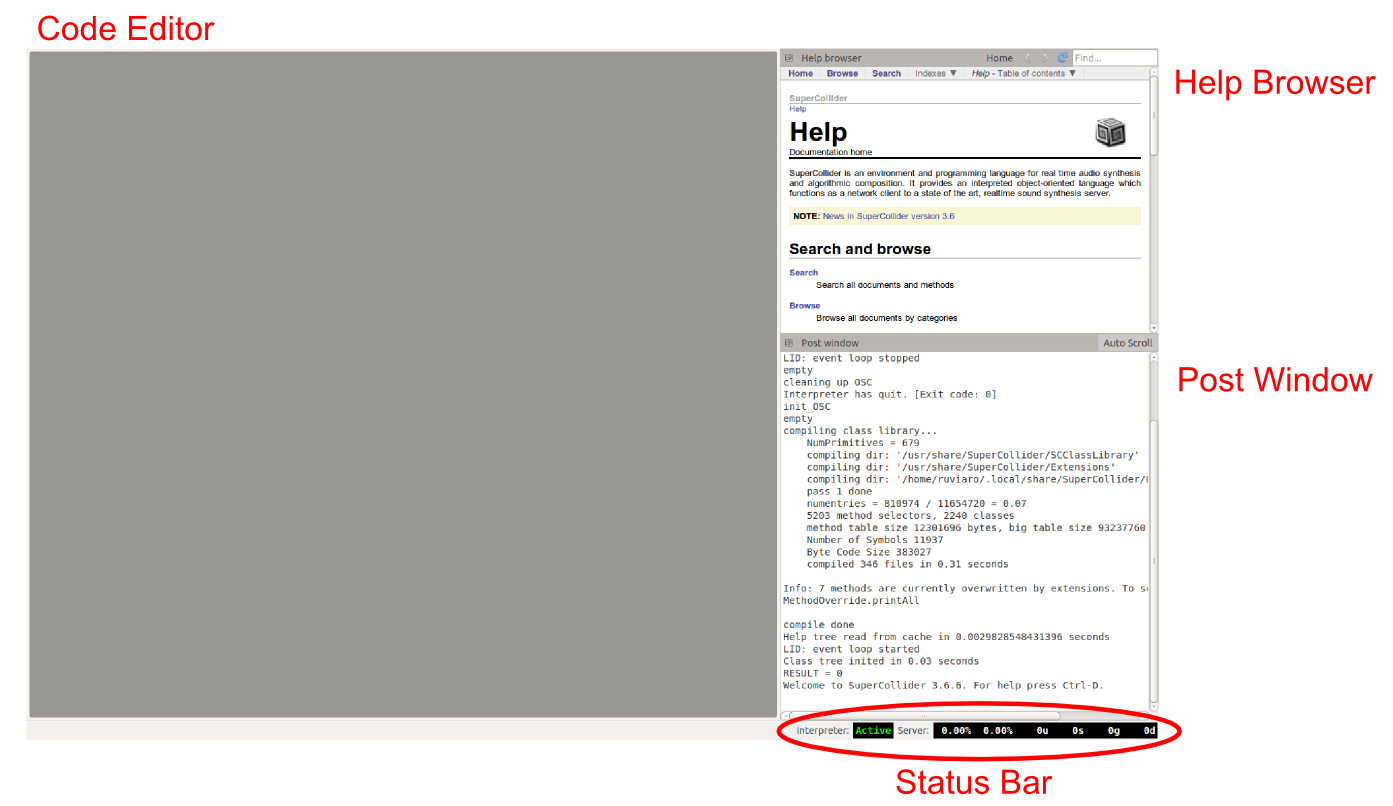
\includegraphics[width=0.7\columnwidth]{fig-supercollider-ide-2.png}}}
\caption{A interface IDE do SuperCollider.}
\label{fig:scidegui}
\end{figure}

O que é a IDE do SuperCollider? É um "ambiente de programação multiplataforma desenvolvido especificamente para o SuperCollider (\dots), 
fácil de começar a usar, prática de lidar e adornada com características poderosas para programadores experientes. Ela também é bastante personalizável. Roda igualmente bem e tem quase a mesma aparência no 
Mac OSX, Linux and Windows."\footnote{Citado da documentação do SuperCollider: \url{http://doc.sccode.org/Guides/SCIde.html}. Visite esta página para aprender mais sobre a interface da IDE.}

As principais partes que você vê são o Editor de Código, o Navegador de Ajuda ("Help browser") e a Janela de Postagem ("Post window"). Se você não estiver vendo qualquer uma dessas quando abre o Super Collider, simplesmente vá para o menu View$\rightarrow$Docklets (é onde você pode mostrar ou esconder cada uma delas). Há também a Barra de Status, sempre localizada no canto inferior direito da janela.

Sempre mantenha a Post window visível, mesmo se você ainda não entende todas as coisas que são mostradas ali. A Post window mostra as reações do programa aos seus comandos: resultados da execução de códigos, notificações diversas, avisos, erros, etc.

\bigskip
\todo[inline, color=green!40]{ 
DICA: Você pode aumentar ou reduzir temporariamente o tamanho da fonte do editor com os atalhos [Ctrl++] e [Ctrl+-] (ou seja, a tecla control junto com as teclas de mais ou menos, respectivamente). Se você está em um laptop que não tem uma tecla de mais de verdade, use [Ctrl+shift+=].}
\bigskip



\section{Servidor e Linguagem}

Na Barra de Status você pode ver as palavras "Interpreter" ("Interpretador") e "Server" ("Servidor"). Por definição, o Interpretador fica ligado ("Active") na abertura do programa, enquanto o "Servidor" fica desligado (é isso o que todos aqueles zeros querem dizer). O que é o Interpretador é o que é o Servidor?

O SuperCollider, na realidade, é feito de dois aplicativos distintos: o servidor e a linguagem. O servidor é responsável por fazer sons. A linguagem (também chamada \emph{cliente} ou \emph{interpretador}) é usada para controlar o servidor. O primeiro é chamado scsynth (SC-synthesizer) e o segundo, sclang (SC-language). A Barra de Status diz o status (ligado/desligado) de cada um destes dois componentes.

Não se preocupe se esta distinção não faz muito sentido para você agora. As duas principais coisas que você precisa saber neste ponto são:

\begin{enumerate}
\item Tudo o que você digita no SuperCollider está na linguagem do SuperCollider (o cliente): é onde você escreve e executa comandos e vê os resultados na Post window.
\item Tudo o que faz som no SuperCollider está vindo do servidor---o "motor sonoro", por assim dizer---, controlado por você através da linguagem do SuperCollider.
\end{enumerate}

\subsection{Iniciando o Servidor}
Seu programa "Olá Mundo" não produziu som algum: tudo aconteceu na linguagem e o servidor nem chegou a ser usado. O próximo exemplo fará som, então precisamos ter certeza que o Servidor está ligado e funcionando.

O jeito mais fácil de iniciar o servidor é com o atalho [ctrl+B]. Alternativamente, você pode clicar nos zeros da Barra de Status: um menu aparece e uma das opções é "Boot Server" ("Iniciar Servidor"). Você verá alguma atividade na Post Window enquanto o servidor está iniciando. Depois que você tiver iniciado o servidor com sucesso, os números na Barra de Status vão ficar verdes. Você terá de fazer isso todas as vezes que você iniciar o SC, mas apenas uma vez por sessão.



\section{Sua primeira senóide \label{sec:first-sine}}


"Olá, Mundo" é tradicionalmente o primeiro programa que as pessoas criam quando estão aprendendo uma nova linguagem de programação. Você já fez isso no SuperCollider.

Criar uma onda senoidal simples talvez seja o "Olá, Mundo" das linguagens de programação para música. Vamos direto à senóide então. Digite e execute a seguinte linha de código. Cuidado---o volume pode ser alto. Abaixe todo seu volume do computador, execute a linha e aumente o volume devagar.
 
\begin{lstlisting}[style=SuperCollider-IDE, basicstyle=\scttfamily\footnotesize]
{SinOsc.ar}.play;
\end{lstlisting}
 

Trata-se de uma senoide bela, suave, contínua e talvez um pouco entediante. Você pode parar o som com [ctrl+.] (ou seja, a tecla \emph{control} junto com a tecla de \emph{ponto final}.) Memorize esta combinação de teclas, porque você a utilizará muito para interromper todo e qualquer som no SC.

\bigskip
\todo[inline, color=green!40]{ 
DICA: Em uma linha separada, digite e execute \texttt{s.volume.gui} se você quiser um slider gráfico para controlar o volume da saída do SuperCollider.
}
\bigskip

Agora vamos tornar esta senoide um pouco mais interessante. Digite isto:

 
\begin{lstlisting}[style=SuperCollider-IDE, basicstyle=\scttfamily\footnotesize ]
{SinOsc.ar(LFNoise0.kr(10).range(500, 1500), mul: 0.1)}.play;
\end{lstlisting}
 

Lembre-se, basta deixar o cursor em qualquer lugar da linha e apertar [ctrl+Enter] para executar. Ou, se preferir, você pode também selecionar toda a linha antes de executá-la.

 
\bigskip
\todo[inline, color=green!40]{ 
DICA: Digitar os próprios exemplos é uma grande ferramenta de aprendizagem. Isso irá ajudar a criar confiança e familiaridade com a linguagem. Ao ler tutoriais em formato digital, você pode às vezes sentir uma certa preguiça e ser tentado a copiar e colar o código dos exemplos. Evite fazer isso: você aprenderá melhor se digitar tudo por conta própria, ao menos nos primeiros estágios da sua aprendizagem com o SC.
}

\section{Error messages}

No sound when you evaluated the last example? If so, your code probably had a typo: a wrong character, a missing comma or parenthesis, etc. When something goes wrong in your code, the Post window gives you an error message. Error messages can be long and cryptic, but don't panic: with time you will learn how to read them. A short error message could look like this:

\begin{verbatim}
ERROR: Class not defined.
  in file 'selected text'
  line 1 char 19:

  {SinOsc.ar(LFNoiseO.kr(12).range(400, 1600), mul: 0.01)}.play; 
                     
-----------------------------------
nil
\end{verbatim}

This error message says, ``Class not defined,'' and points to the approximate location of the error (``line 1 char 19''). Classes in SC are those blue words that start with a capital letter (like \texttt{SinOsc} and \texttt{LFNoise0}). It turns out this error was due to the user typing LFNoiseO with a capital letter ``O'' at the end. The correct class is LFNoise0, with the number zero at the end. As you can see, attention to detail is crucial.

If you have an error in your code, proofread it, change as needed, and try again until it's fixed. If you had no error at first, try introducing one now so you can see how the error message would look like (for example, remove a comma).

\bigskip
\todo[inline, color=green!40]{ 
TIP: Learning SuperCollider is like learning another language like German, Portuguese, Japanese\dots \  just keep trying to speak it, work on expanding your vocabulary, pay attention to grammar and syntax, and learn from your mistakes. The worst it can happen here is to crash SuperCollider. Not nearly as bad as taking the wrong bus in São Paulo because of a mispronounced request for directions.
}
\section{Mudando parâmetros}

Aqui temos um bom exemplo adaptado do primeiro capítulo do The SuperCollider Book.\footnote{
Wilson, S. and Cottle, D. and Collins, N. (Editors). The SuperCollider Book, MIT Press, 2011, p. 5. Diversas coisas neste tutorial foram emprestadas, adaptadas ou inspiradas pelo excelente “Beginner’s Tutorial” de David Cottle, que é o primeiro capítulo do livro, mas---diferentemente dele--aqui assumimos que o leitor tenha pouca familiaridade com a computer music e apresentamos a família Pattern como espinha dorsal da abordagem pedagógica.
} Da mesma forma que em exemplos anteriores, não se preocupe em entender tudo. Apenas aprecie o resultado sonoro e brinque com os números.


\begin{lstlisting}[style=SuperCollider-IDE, basicstyle=\scttfamily\footnotesize]
{RLPF.ar(Dust.ar([12, 15]), LFNoise1.ar([0.3, 0.2]).range(100, 3000), 0.02)}.play;
\end{lstlisting}

Pare o som, mude alguns números e rode novamente. Por exemplo, o que acontece quando você substitui os números 12 e 15 por valores mais baixos, entre 1 e 5? Depois de \texttt{LFNoise1}, que tal se em vez de 0.3 e 0.2 você tentasse algo como 1 ou 2?Mude um de cada vez. Compare o novo som com o som anterior, escute as diferenças. Veja se você consegue entender qual número está controlando o quê. Esta é uma maneira divertida de explorar o SuperCollider: pegue um trecho de código que faça algo interessante e experimente com os parâmetros para criar variações. Mesmo se você não entender completamente o papel individual de cada número, ainda assim pode encontrar resultados sonoros interessantes.

\bigskip 
\todo[inline, color=green!40]{ 
DICA: Como qualquer software, lembre-se de salvar frequentemente o seu trabalho com [ctrl+S]! Quanto estiver trabalhando em tutoriais como esse, você muitas vezes vai chegar a sons interessantes experimentando com os exemplos fornecidos. Quando você quer guardar algo que você gosta, copie o código para um novo documento e salve-o. Perceba que todo arquivo do SuperCollider tem a extensão .scd, que quer dizer "SuperCollider Document."
}

\section{Comments}

All text in your code that shows in red color is a \emph{comment}. If you are new to programming languages, comments are a very useful way to document your code, both for yourself and for others who may have to read it later. Any line that starts with a double slash is a comment. You can write comments right after a valid line of code; the comment part will be ignored when you evaluate. In SC we use a semicolon to indicate the end of a valid statement.

\begin{lstlisting}[style=SuperCollider-IDE, basicstyle=\scttfamily\footnotesize]
2 + 5 + 10 - 5; // just doing some math

rrand(10, 20); // generate a random number between 10 and 20
\end{lstlisting}

You can evaluate a line even if your cursor is in the middle of the comment after that line. The comment part is ignored. The next two paragraphs will be written as ``comments'' just for the sake of the example.

 
\begin{lstlisting}[style=SuperCollider-IDE, basicstyle=\scttfamily\footnotesize]
// You can quickly comment out one line of code using the shortcut [ctrl+/].
"Some SC code here...".postln;
2 + 2;

// If you write a really long comment, your text may break into what looks like a new line that does *not* start with a double slash. That still counts as a single line of comment.

/* Use "slash + asterisk" to start a longer comment with several lines. Close the big comment chunk with "asterisk + slash." The shortcut mentioned above also works for big chunks: simply select the lines of code you want to comment out, and hit [ctrl+/]. Same to un-comment. */
\end{lstlisting}
\section{Precedência}

O SuperCollider segue a ordem de precedência da esquerda para a direita, independente da operação. Isso significa, por exemplo, que multiplicação \emph{não} acontece primeiro:

\begin{lstlisting}[style=SuperCollider-IDE, basicstyle=\scttfamily\footnotesize]
// No colégio, o resultado era 9; no SC é 14:
5 + 2 * 2; 
//Use parênteses para forçar uma ordem de operações específica:
5 + (2 * 2); // igual a 9.
\end{lstlisting}

Quando se combina mensagens e operações binárias, mensagens assumem precedência. Por exemplo, em \texttt{5 + 2.squared}, a elevação ao quadrado acontece primeiro.

\section{The last thing always gets posted}

A small but useful detail to understand: SuperCollider, by default, always posts to the Post window the result of whatever was the \emph{last thing to be evaluated}. This explains why your Hello World code prints twice when you evaluate. Type the following lines onto a new document, then select all with [ctrl+A] and evaluate all lines at once:

\begin{lstlisting}[style=SuperCollider-IDE, basicstyle=\scttfamily\footnotesize]
"First Line".postln;
"Second Line".postln;
(2 + 2).postln;
3 + 3;
"Finished".postln;
\end{lstlisting}

All five lines are executed by SuperCollider. You see the result of \texttt{2 + 2} in the Post window because there was an explicit \texttt{postln} request. The result of \texttt{3 + 3} was calculated, but there was no request to post it, so you don't see it. Then the command of the last line is executed (the word ``Finished'' gets posted due to the \texttt{postln} request). Finally, the result of the very last thing to be evaluated is posted by default: in this case, it happened to be the word ``Finished.''
\section{Blocos de código}
\label{sec:code-block}


Selecionando múltiplas linhas de um código antes de rodá-lo pode ser tedioso. Uma maneira muito mais fácil de rodar toda uma porção de código ao mesmo tempo é criar um \textit{bloco de código}: simplesmente coloque dentro de parênteses todas as linhas de código que você quer rodar juntas. Aqui temos um exemplo:


\begin{lstlisting}[style=SuperCollider-IDE, basicstyle=\scttfamily\footnotesize]
(
// Um pequeno poema
"Hoje é domingo".postln;
"Pé de cachimbo".postln;
"O cachimbo é de ouro".postln;
"Bate no touro".postln;
)
\end{lstlisting}

Os parênteses externos delimitam o bloco de código. Desde que que o cursor esteja em qualquer lugar dentro dos parênteses, um único [ctrl+Enter] rodará as linhas para você (elas serão executadas na ordem de cima para baixo, mas isso é tão rápido que parece simultâneo).

Usar blocos de código poupa o trabalho de ter de selecionar todas as linhas novamente a cada vez que você quiser mudar algo e rodar novamente. Por exemplo mude algumas das palavras entre aspas e pressione [ctrl+Enter] logo após fazer a mudança. Todo o bloco de código é rodado sem que você tenha que selecionar manualmente todas as linhas. O SuperCollider ressalta o bloco por um segundo para dar uma indicação visual de o que está sendo executado.

\section{Como limpar a Post window}

Este é um comando tão útil para maníacos por limpeza que merece uma seção só pra ele: [ctrl+shift+P]. Execute esta linha e experimente limpar a Post window em seguida:

 
\begin{lstlisting}[style=SuperCollider-IDE, basicstyle=\scttfamily\footnotesize]
100.do({"Imprima esta linha um monte de vezes...".scramble.postln});
\end{lstlisting}
 
Não precisa agradecer.


\section{Recording the output of SuperCollider}

Soon you will want to start recording the sound output of your SuperCollider patches. Here's a quick way:
 
\begin{lstlisting}[style=SuperCollider-IDE, basicstyle=\scttfamily\footnotesize]
// QUICK RECORD
// Start recording:
s.record;
// Make some cool sound
{Saw.ar(LFNoise0.kr([2, 3]).range(100, 2000), LFPulse.kr([4, 5]) * 0.1)}.play;
// Stop recording:
s.stopRecording;
// Optional: GUI with record button, volume control, mute button:
s.makeWindow;
\end{lstlisting}
 
The Post Window shows the path of the folder where the file was saved. Find the file, open it with Audacity or similar program, and verify that the sound was indeed recorded. For more info, look at the ``Server'' Help file (scroll down to ``Recording Support''). Also online at \url{http://doc.sccode.org/Classes/Server.html}.
\section{Variáveis}
\label{sec:variables}

Você pode guardar números, palavras, unidades geradoras, funções ou blocos inteiros de código em variáveis. Variáveis podem ser letras minúsculas simples ou palavras escolhidas por você. Usamos o sinal de igual (=) para "atribuir" variáveis. Rode estas linhas uma de cada vez e observe a Post window:

 
\begin{lstlisting}[style=SuperCollider-IDE, basicstyle=\scttfamily\footnotesize]
x = 10;
y = 660;
y; // confira o que está aqui dentro
x;
x + y;
y - x;
\end{lstlisting}
 

A primeira linha atribui o número 10 à variável \texttt{x}. A segunda linha coloca 660 na variável \texttt{y}. As próximas duas linhas provam que estas letras agora "contêm" estes números (os dados). Finalmente, as duas últimas linhas mostram que podemos usar as variáveis para fazer qualquer operação com os dados guardados nelas.

Letras minúsculas de \texttt{a} a \texttt{z} podem ser utilizadas a qualquer momento como variáveis no SuperCollider. A única letra simples que comumente não se usa é \texttt{s}, que por convenção é reservada para representar o Servidor. Qualquer coisa pode entrar em uma variável:
 
\begin{lstlisting}[style=SuperCollider-IDE, basicstyle=\scttfamily\footnotesize]
a = "Olá Mundo"; // uma cadeia de caracteres
b = [0, 1, 2, 3, 5]; // uma lista
c = Pbind(\note, Pwhite(0, 10), \dur, 0.1); // você aprenderá tudo sobre Pbind mais adiante, não se preocupe

// ...e agora você pode utilizá-las como você utilizaria os dados originais:
a.postln; // poste-a
b + 100; // faça contas
c.play; // toque aquele Pbind
d = b * 5; // pegue b, multiplique por 5 e atribua o resultado a uma nova variável
\end{lstlisting}

Muitas vezes fará mais sentido dar nomes melhores para suas variáveis, para ajudar a lembrar o que elas representam no seu código. Você pode usar um $\sim$ (til) para declarar uma variável com um nome mais longo. Note que não há espaço entre o til e o nome da variável.

\begin{lstlisting}[style=SuperCollider-IDE, basicstyle=\scttfamily\footnotesize]
~minhasFreqs = [415, 220, 440, 880, 220, 990];
~minhasDurs = [0.1, 0.2, 0.2, 0.5, 0.2, 0.1];

Pbind(\freq, Pseq(~minhasFreqs), \dur, Pseq(~minhasDurs)).play;
\end{lstlisting}
 

Nomes de variáveis devem começar com letras minúsculas depois do til. Você pode usar números, underscores e letras maiúsculas no meio do nome, somente não como primeiro caracter. Todos os caracteres têm de ser contíguos (sem espaços ou pontuação). Resumindo, atenha-se a letras e números e underscores ocasionais, evitando todos os outros caracteres ao nomear suas variáveis. \texttt{$\sim$minhasFreqs}, \texttt{$\sim$aMelhorSenoide} e \texttt{$\sim$banana\_3} são nomes válidos. \texttt{$\sim$MinhasFreqs}, \texttt{$\sim$aMelhor\&*\#\@Senoide} e \texttt{$\sim$banana!!!} vão estragar o seu dia.

Há dois tipos de variáveis que você pode criar: variáveis "globais" e variáveis locais.

\subsection{"Global" vs. Local}

As variáveis que vimos até agora (letras minúsculas de \texttt{a} a \texttt{z} e aquelas começando com o caracter til ($\sim$)) são genericamente chamadas "variáveis globais", porque uma vez declaradas, funcionarão "globalmente" em qualquer lugar no patch, em outros patches e mesmo em outros documentos do SC, até que você saia do SuperCollider.\footnote{Tecnicamente falando, variáveis começando com um til são chamadas variáveis de Ambiente ("Environment") e variáveis de letras minúsculas (de a a z) são chamadas variáveis do Interpretador. Iniciantes no SuperCollider não precisam se preocupar com estas distinções, mas mantenha-as em mente para o futuro. O Capítulo 5 do The SuperCollider Book explica a diferença em detalhes.}

Variáveis locais, por outro lado, são declaradas com a palavra-chave específica \texttt{\textbf{var}} no início de uma linha. Você pode atribuir um valor inicial para uma variável no momento de sua declaração (\texttt{\textbf{var} tangerina = 4}). Variáveis locais apenas existem dentro do escopo de seu bloco de código.

Aqui está um exemplo simples comparando os dois tipos de variáveis. Execute linha a linha e observe a Post window.

 
\begin{lstlisting}[style=SuperCollider-IDE, basicstyle=\scttfamily\footnotesize]
// Variáveis de Ambiente
~abacates = 4;
~laranjas = 5;
~tangerinas = 2;
~bananas = 1;

["Cítricos", ~laranjas + ~tangerinas];
["Não-Cítricos", ~bananas + ~abacates];

// Variáveis locais: válidas apenas dentro do bloco de código.
// Execute o bloco uma vez e observe o Post window:
(
var jacas = 4, laranjas = 3, tangerinas = 8, bananas = 10;
["Frutas cítricas", laranjas + tangerinas].postln;
["Frutas Não-cítricas", bananas + jacas].postln;
"Fim".postln;
)

~abacates; // variável ainda existe
jacas; // variável não existe mais
\end{lstlisting}

\subsection{Reatribuição}

Uma última coisa útil de se entender sobre variáveis é que elas podem ser \emph{reatribuídas}: você pode dar-lhes um novo valor a qualquer momento.

\begin{lstlisting}[style=SuperCollider-IDE, basicstyle=\scttfamily\footnotesize]
// Atribua uma variável
a = 10 + 3;
a.postln; // verifique
a = 999; // reatribua a variável (dê-lhe um novo valor)
a.postln; // verifique: o valor antigo se foi.
\end{lstlisting}

Uma prática muito comum que pode parecer um pouco confusa para iniciantes é quando \emph{a própria variável é usada na sua própria reatribuição}. Dê uma olhada neste exemplo:

\begin{lstlisting}[style=SuperCollider-IDE, basicstyle=\scttfamily\footnotesize]
x = 10; // atribua 10 à variável x
x = x + 1; // atribua x + 1 à variável x
x.postln; // verifique
\end{lstlisting}

A maneira mais fácil de entender essa última linha é lê-la da seguinte forma: "pegue o valor atual da variável x, adicione 1 a ela e atribua este novo resultado à variável x". No fundo, não é tão complicado e você verá mais tarde como isso pode ser útil.\footnote{Este exemplo claramente demonstra que o sinal de igual, em programação, não é o mesmo sinal de igual que você aprendeu em matemática. Em matemática, $x = x + 1$ é impossível (um número não pode ser igual a si mesmo mais um). Já em uma linguagem de programação como o SuperCollider, o sinal de igual pode ser entendido como um tipo de ação: \emph{pegue o resultado da expressão à direita do símbolo e o "atribua" à variável ao lado esquerdo}.}


% PART II
\newpage
\part{PATTERNS}
\section{A família Pattern}

Vamos experimentar algo diferente agora. Digite e rode esta linha de código:

\begin{lstlisting}[style=SuperCollider-IDE, basicstyle=\scttfamily\footnotesize]
Pbind(\degree, Pseries(0, 1, 30), \dur, 0.05).play;
\end{lstlisting}

\subsection{Conheça o Pbind}

\texttt{Pbind} é um membro da família Pattern ("padrão" ou "modelo") no SuperCollider. O P maiúsculo no \texttt{Pbind} e \texttt{Pseries} remete a \emph{Pattern}; em breve teremos o prazer de conhecer outros membros da família. Por ora, vamos focar somente somente no \texttt{Pbind}. Experimente este exemplo reduzido ao mínimo:

\begin{lstlisting}[style=SuperCollider-IDE, basicstyle=\scttfamily\footnotesize]
Pbind(\degree, 0).play;
\end{lstlisting}

A única coisa que esta linha de código faz na vida é tocar a nota \emph{dó central}, uma vez por segundo. A palavra-chave \texttt{\textbackslash degree} se refere a graus de uma escala e o número 0 representa o primeiro grau da escala (uma escala de Dó Maior é subentendida, então esta é a própria nota dó). Note que o SuperCollider começa a contar as coisas do 0 e não do 1. Em uma linha simples como esta acima, as notas dó, ré, mi, fá, sol\dots seriam representadas pelos números 0, 1, 2, 3, 4\dots Tente mudar o número e perceba como a nota muda quando você reexecuta. Você também pode escolher notas abaixo do dó central (por exemplo, -2 é a nota lá abaixo do dó central). Resumindo, apenas imagine que o dó central do piano é 0 e conte teclas brancas para cima ou para baixo (números positivos ou negativos) para obter qualquer outra nota.

Agora brinque um pouco com a duração das notas. \texttt{Pbind} usa a palavra-chave \texttt{\textbackslash dur} para especificar durações em segundos:

\begin{lstlisting}[style=SuperCollider-IDE, basicstyle=\scttfamily\footnotesize]
Pbind(\degree, 0, \dur, 0.5).play;
\end{lstlisting}

Claro que isso ainda é muito rígido e inflexível---sempre a mesma nota, sempre a mesma duração. Não se preocupe: as coisas vão esquentar logo, logo.
\subsection{Pseq}

Vamos agora tocar várias notas em sequência, como uma escala. Vamos também diminuir a duração das notas para 0.2 segundos.
 
\begin{lstlisting}[style=SuperCollider-IDE, basicstyle=\scttfamily\footnotesize]
Pbind(\degree, Pseq([0, 1, 2, 3, 4, 5, 6, 7], 1), \dur, 0.2).play;
\end{lstlisting}

Esta linha introduz um novo membro da família Pattern: \texttt{Pseq}. Como o nome sugere, este Pattern lida com sequências. Tudo que um \texttt{Pseq} precisa para tocar uma sequência é:
\begin{itemize}
\item uma lista de itens entre colchetes []
\item um número de repetições.
\end{itemize} 

No exemplo, a lista é \texttt{[0, 1, 2, 3, 4, 5, 6, 7]} e o número de repetições é \texttt{1}. Este \texttt{Pseq} simplesmente diz: "toque todos os itens da lista, na sequência, uma vez". Repare que estes dois elementos, lista e número de repetições, estão dentro dos parênteses que pertencem ao \texttt{Pseq} e são separados por uma vírgula.

Veja também onde o \texttt{Pseq} aparece no interior do \texttt{Pbind}: é colocado como valor de \texttt{\textbackslash degree}. Isso é importante: em vez de fornecer um número único e fixo para o grau da escala (como no nosso primeiro \texttt{Pbind} simples), \emph{estamos fornecendo todo um Pseq: uma receita para uma sequência de números}. Com isto em mente, podemos facilmente expandir esta ideia e usar outro Pseq para controlar também as durações.
 
\begin{lstlisting}[style=SuperCollider-IDE, basicstyle=\scttfamily\footnotesize]
Pbind(\degree, Pseq([0, 1, 2, 3, 4, 5, 6, 7], 5), \dur, Pseq([0.2, 0.1, 0.1, 0.2, 0.2, 0.35], inf)).play;
\end{lstlisting}
 
O que está acontecendo neste exemplo? Primeiro, mudamos o número de repetições do primeiro \texttt{Pseq} para 5, de modo que toda a escala vai tocar cinco vezes. Segundo, substituímos o valor de \texttt{\textbackslash dur}, antes fixo em 0.2, por um outro \texttt{Pseq}. Este novo \texttt{Pseq} tem uma lista de seis itens: \texttt{[0.2, 0.1, 0.1, 0.2, 0.2, 0.35]}. Estes números se tornam valores de duração das notas resultantes. O valor de \texttt{repeats} deste segundo \texttt{Pseq} é definido como \texttt{inf}, que quer dizer "infinito". Isso sgnifica que o \texttt{Pseq} não tem limite no número de vezes que ele pode repetir esta sequência. Então o \texttt{Pbind} toca para sempre? Não: ele para depois que o \emph{outro} \texttt{Pseq} terminou seu trabalho, isto é, depois que a sequência de graus de escala foi tocada 5 vezes.

Finalmente, o exemplo tem um total de oito notas diferentes (a lista no primeiro \texttt{Pseq}), enquanto há apenas seis valores para duração (segundo \texttt{Pseq}). Quando você fornece sequências de tamanhos diferentes como estas, o \texttt{Pbind} simplesmente as faz circular o quanto for preciso.

Responda estas perguntas para praticar o que você aprendeu:
\begin{itemize}
\item Experimente o número 1 em vez de inf como o argumento \texttt{repeats} do segundo \texttt{Pseq}. O que acontece?
\item Como você pode fazer este Pbind tocar para sempre?
\end{itemize}

Soluções estão no final do livro.\endnote{Primeira pergunta: quando você usa o número 1 em vez de \texttt{inf} como o argumento \texttt{repeats} do segundo \texttt{Pseq}, o Pbind para depois que 6 notas foram tocadas (isto é, depois que uma sequência completa de valores de duração foi tocada). Segunda questão: para fazer o Pbind tocar para sempre, simplesmente use \texttt{inf} como valor para \texttt{repeats} em todos os Patterns internos.}

\subsection{Deixe seu código mais legível}

Você deve ter percebido que a linha de código acima é um tanto longa. De fato, ela é tão longa que quebra em uma nova linha, mesmo que tecnicamente se trate de um enunciado único. Linhas de código longas podem ser confusas de ler. Para evitar isso, é uma prática comum quebrar o código em várias linhas indentadas; com o objetivo de torná-lo o mais claro e inteligível possível. O mesmo \texttt{Pbind} pode ser escrito assim:

\begin{lstlisting}[style=SuperCollider-IDE, basicstyle=\scttfamily\footnotesize]
(
Pbind(
	\degree, Pseq([0, 1, 2, 3, 4, 5, 6, 7], 5),
	\dur, Pseq([0.2, 0.1, 0.1, 0.2, 0.2, 0.35], inf)
).play;
)
\end{lstlisting}

De agora em diante, adquira o hábito de escrever seus \texttt{Pbind}s deste jeito. Escrever código com uma aparência arrumada e bem organizada vai ajudá-lo bastante no aprendizado do SuperCollider.

Além disso, perceba que envolvemos este \texttt{Pbind} dentro de parênteses para criar um bloco de código (lembra-se da seção \ref{sec:code-block}?): como ele não está mais em uma única linha, precisamos fazer isso para conseguir rodá-lo todo de uma vez. Lembre-se que o cursor precisa estar em algum lugar no interior do bloco antes de executá-lo.


\subsection{Quatro maneiras de especificar alturas}

\texttt{Pbind} aceita outras maneiras de especificar alturas, não apenas graus de escala.
\begin{itemize}
\item Se você quiser usar todas as doze notas cromáticas (teclas brancas e pretas do piano), você pode usar \texttt{\textbackslash note} em vez de \texttt{\textbackslash degree}. 0 continuará representando o dó central, mas agora os números incluem as teclas pretas do piano (0=dó central, 1=dó$\sharp$, 2=ré, etc).
\item Se você preferir usar a numeração de notas MIDI, use \texttt{\textbackslash midinote} (60=dó central, 61=dó$\sharp$, 62=ré, etc).
\item Finalmente, se você quiser especificar frequências diretamente em Herz, use \texttt{\textbackslash freq}.
\end{itemize}

Veja a figura \ref{fig:scale-degrees} para uma comparação dos quatro métodos.

\begin{figure}[h]
\centering
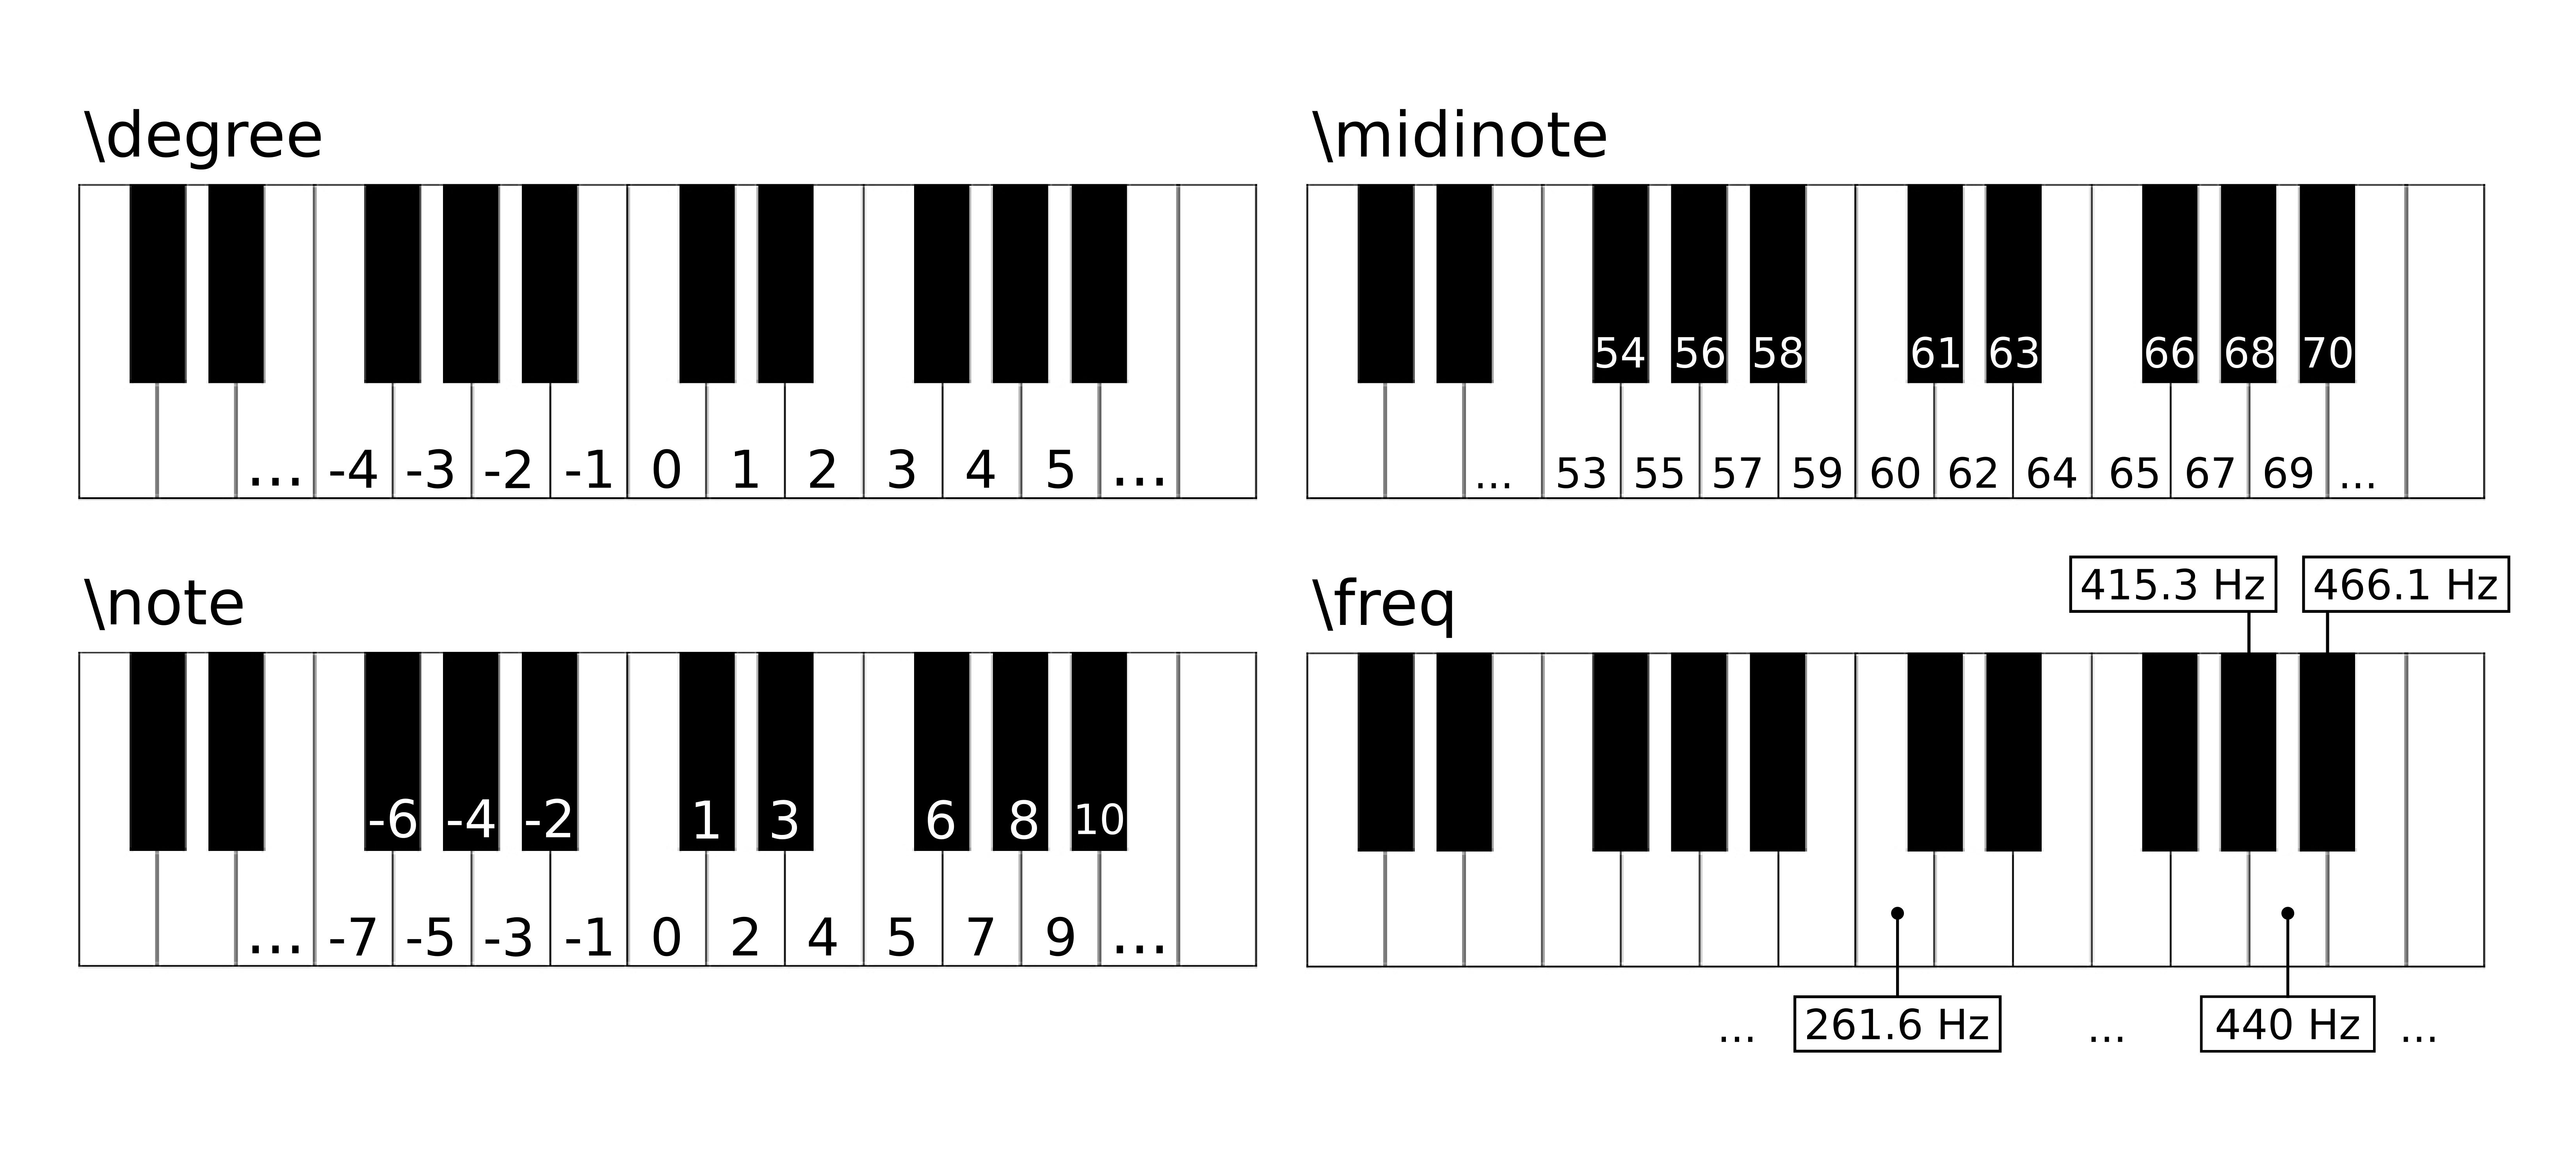
\includegraphics[scale=0.4]{fig-piano-keyboard-degree-note-midinote-freq.png}
\caption{Comparando graus de escala, números de nota, notas MIDI e frequências}
\label{fig:scale-degrees}
\end{figure}

No próximo exemplo, quatro Pbinds vão tocar a mesma nota: o lá acima do dó central (lá 4).

\begin{lstlisting}[style=SuperCollider-IDE, basicstyle=\scttfamily\footnotesize]
Pbind(\degree, 5).play;
Pbind(\note, 9).play;
Pbind(\midinote, 69).play;
Pbind(\freq, 440).play;
\end{lstlisting}


\bigskip
\todo[inline, color=green!40]{
DICA: Lembre-se que cada maneira de especificar alturas requer números em âmbitos dife-rentes. Uma lista de números como \texttt{[-1, 0, 1, 3]} faz sentido para \texttt{\textbackslash degree} e \texttt{\textbackslash note}, mas não faz sentido para \texttt{\textbackslash midinote} ou \texttt{\textbackslash freq}. A tabela abaixo compara alguns valores usando o teclado do piano como referência.
}
\bigskip


\begin{tabular}{|l|c|c|c|c|c|}
\hline 
  & \textbf{lá 0 (nota mais grave do piano)} & \textbf{dó 4} & \textbf{lá 4} & \textbf{dó 5} & \textbf{dó 8} \\ 
\hline 
\texttt{\textbackslash degree} & -23 & 0 & 5 & 7 & 21 \\
\hline
\texttt{\textbackslash note} & -39 & 0 & 9 & 12 & 48 \\
\hline
\texttt{\textbackslash midinote} & 21 & 60 & 69 & 72 & 108 \\
\hline
\texttt{\textbackslash freq} & 27.5 & 261.6 & 440 & 523.2 & 4186 \\
\hline
\end{tabular}
\bigskip


\subsection{Mais palavras-chave: amplitude e legato}

O novo exemplo introduz duas novas palavras-chave: \texttt{\textbackslash amp} e \texttt{\textbackslash legato}, que definem a amplitude dos eventos e a quantidade de legato entre as notas. Perceba como o código fica bem mais fácil de ler, graças a uma boa indentação e distribuição em várias linhas. Parênteses externos (no topo e embaixo) são usados para delimitar um bloco de código a ser executado de uma vez.

 
\begin{lstlisting}[style=SuperCollider-IDE, basicstyle=\scttfamily\footnotesize]
(
Pbind(
	\degree, Pseq([0, -1, 2, -3, 4, -3, 7, 11, 4, 2, 0, -3], 5),
	\dur, Pseq([0.2, 0.1, 0.1], inf),
	\amp, Pseq([0.7, 0.5, 0.3, 0.2], inf),
	\legato, 0.4
).play;
)
\end{lstlisting}
 

\texttt{Pbind} tem muitas destas palavras-chave pré-definidas e, com o tempo, você aprenderá mais delas. Por agora, vamos nos centrar em apenas algumas---uma para altura (com as opções de \texttt{\textbackslash degree}, \texttt{\textbackslash note}, \texttt{\textbackslash midinote} ou \texttt{\textbackslash freq}), uma para durações (\texttt{\textbackslash dur}), uma para amplitude (\texttt{\textbackslash amp}) e uma para legato (\texttt{\textbackslash legato}). Durações estão em tempos (neste caso, 1 batida por segundo, que é o padrão); a amplitude deve estar entre 0 e 1 (0 = silêncio, 1 = muito alto); e o legato funciona melhor com valores entre 0.1 e 1 (se você não tem certeza o que o legato faz, simplesmente experimente o exemplo acima com 0.1, depois 0.2, depois 0.3, até chegar no 1 e ouça os resultados).

Tome o último exemplo como um  ponto de partida e crie novos \texttt{Pbind}s. Mude a melodia. Introduza novas listas de durações e amplitudes. Experimente usar \texttt{\textbackslash freq} para alturas. Lembre, você sempre pode usar um número fixo para qualquer um destes parâmetros, se quiser. Por exemplo, se você quer que todas as notas da sua melodia tenham 0.2 segundos de duração, não há porque escrever \texttt{Pseq[0.2, 0.2, 0.2, 0.2\dots}, nem mesmo \texttt{Pseq([0.2], inf)}---simplesmente remova toda a estrutura do \texttt{Pseq} e escreva 0.2 no lugar.

\subsection{Prand}

\texttt{Prand} é um parente próximo do \texttt{Pseq}. Ele também aceita uma lista e um número de repetições. Mas em vez de ir tocando a lista na sequência, \texttt{Prand} \emph{escolhe um item aleatório da lista a cada vez}. Experimente:

 
\begin{lstlisting}[style=SuperCollider-IDE, basicstyle=\scttfamily\footnotesize]
(
Pbind(
	\degree, Prand([2, 3, 4, 5, 6], inf),
	\dur, 0.15,
	\amp, 0.2,
	\legato, 0.1
).play;
)
\end{lstlisting}
 

Substitua \texttt{Prand} pelo \texttt{Pseq} e compare os resultados. Agora experimente usar \texttt{Prand} para durações, amplitudes e legato.

\subsection{Pwhite}

Outro membro popular da família Pattern é o \texttt{Pwhite}. É um gerador de números aleatórios de distribuição uniforme (o nome vem de "white noise", ruído branco). Por exemplo, \texttt{Pwhite(100, 500)} irá fornecer números aleatórios entre 100 e 500.
 
\begin{lstlisting}[style=SuperCollider-IDE, basicstyle=\scttfamily\footnotesize]
(
Pbind(
	\freq, Pwhite(100, 500),
	\dur, Prand([0.15, 0.25, 0.3], inf),
	\amp, 0.2,
	\legato, 0.3
).trace.play;
)
\end{lstlisting}
 

O exemplo acima também mostra outro truque útil: a mensagem \texttt{trace} logo antes de \texttt{play}. Isso imprime na Post window os valores selecionados em cada evento. Muito útil para corrigir problemas ou simplesmente para entender o que está acontecendo!

Preste atenção nas diferenças entre \texttt{Pwhite} e \texttt{Prand}: mesmo que ambos tenham a ver com aleatoriedade, eles aceitam argumentos distintos e fazem coisas diferentes. Dentro dos parênteses do \texttt{Pwhite} você só precisa fornecer um limite mínimo e máximo: \texttt{Pwhite(mínimo, máximo)}. Números aleatórios serão escolhidos no interior deste âmbito. \texttt{Prand}, por outro lado, aceita uma lista de itens (necessariamente entre colchetes) e um número de repetições: \texttt{Prand([lista, de, itens], repetições)}. Itens aleatórios serão escolhidos \emph{desta lista}.

Explore ambos e confirme que você entendeu completamente a diferença.


\bigskip
\todo[inline, color=green!40]{ 
DICA: Um \texttt{Pwhite} com dois números inteiros vai gerar somente números inteiros. Por exemplo, \texttt{Pwhite(100, 500)} vai gerar números como 145, 568, 700, mas não 145.6, 450.32, etc. Se você quer incluir números decimais no resultado, escreva \texttt{Pwhite(100, 500.0)}. Isso é muito útil para, digamos, amplitudes: se você escreve \texttt{Pwhite(0, 1)} vai obter apenas 0 ou 1, mas escreva \texttt{Pwhite(0, 1.0)} e você terá todos os resultados intermediários.
}
\bigskip
 


Tente as seguintes perguntas para testar seu novo conhecimento:

\begin{enumerate}[a)]
\item Qual a diferença entre os resultados de \texttt{Pwhite(0, 10)} e \texttt{Prand([0, 4, 1, 5, 9, 10, 2, 3], inf)}?

\item Se você precisa de um fluxo de números inteiros escolhidos aleatoriamente entre 0 e 100, você poderia usar um \texttt{Prand}?

\item Qual a diferença entre os resultados de \texttt{Pwhite(0, 3)} e \texttt{Prand([0, 1, 2, 3], inf)}? E se você escrever \texttt{Pwhite(0, 3.0)}?

\item  Rode os exemplos abaixo. Usamos \texttt{\textbackslash note} em vez de \texttt{\textbackslash degree} para tocar uma escala de dó menor (que inclui teclas pretas). A lista \texttt{[0, 2, 3, 5, 7, 8, 11, 12]} tem oito números dentro dela, correspondendo às notas dó, ré, mi$\flat$, fá, sol, lá$\flat$, si, dó, mas quantos eventos cada exemplo realmente toca? Por quê?

 
\begin{lstlisting}[style=SuperCollider-IDE, basicstyle=\scttfamily\footnotesize]
// Pseq
(
Pbind(
	\note, Pseq([0, 2, 3, 5, 7, 8, 11, 12], 4),
	\dur, 0.15;
).play;
)

// Pseq
(
Pbind(
	\note, Prand([0, 2, 3, 5, 7, 8, 11, 12], 4),
	\dur, 0.15;
).play;
)

// Pwhite
(
Pbind(
	\note, Pseq([0, 2, 3, 5, 7, 8, 11, 12], 4),
	\dur, Pwhite(0.15, 0.5);
).play;
)
\end{lstlisting}

\end{enumerate}


Respostas ao final deste tutorial.\endnote{\\
a) \texttt{Pwhite(0, 10)} vai gerar qualquer número entre 0 e 10. \texttt{Prand([0, 4, 1, 5, 9, 10, 2, 3], inf)} vai escolher apenas números que estão contidos na lista; note que essa lista tem \emph{alguns} números entre 0 e 10, mas não todos (6, 7, 8 não estão lá, então nunca vão aparecer neste \texttt{Prand}).  \\
b) Tecnicamente você poderia usar um \texttt{Prand} se você fornecer uma lista com todos os números entre 0 e 100, mas faz mais sentido usar um \texttt{Pwhite} para esta tarefa: \texttt{Pwhite(0, 100)}. \\
c) \texttt{Prand([0, 1, 2, 3], inf)} escolhe itens da lista aleatoriamente. \texttt{Pwhite(0, 3)} chega ao mesmo resultado por outros meios: ele gera aleatoriamente números inteiros entre 0 e 3, o que acaba dando o mesmo leque de opções que o \texttt{Prand} acima. No entanto, se você escrever \texttt{Pwhite(0, 3.0)}, o resultado será diferente: como um dos argumentos de entrada do \texttt{Pwhite} está escrito como um decimal (3.0), esse Pwhite produzirá qualquer número decimal entre 0 e 3, como 0.154, 1.0, 1.45, 2.999.
\\
d) O primeiro \texttt{Pbind} toca 32 notes (4 vezes a sequência de 8 notas). O segundo \texttt{Pbind} toca apenas 4 notas: quatro escolhas aleatórias retiradas da lista (lembre-se que o \texttt{Prand}, diferentemente do \texttt{Pseq}, não tem a obrigação de tocar todas as notas da lista: ele vai simplesmente escolher tantos números aleatórios quanto você pedir). O terceiro e último \texttt{Pbind} toca 32 notas, como o primeiro.
}

\bigskip
\todo[inline, color=green!40]{ 
DICA: Um Pbind para de tocar quando o Pattern interno mais curto tiver terminado de tocar (conforme determinado pelo argumento \texttt{repeats} de cada Pattern interno).
}
\bigskip

\subsection{Expandindo seu vocabulário de Patterns}

A partir de agora, você já deve ser capaz de escrever \texttt{Pbind}s simples por conta própria. Você sabe especificar alturas, durações, amplitudes, valores de legato e você sabe como embutir outros Patterns (\texttt{Pseq}, \texttt{Prand}, \texttt{Pwhite}) para gerar mudanças interessantes de parâmetros.

Esta seção irá expandir um pouco seu vocabulário de Patterns. Os exemplos abaixo introduzem seis novos membros da família Pattern. Tente descobrir por você mesmo o que eles fazem. Use as seguintes estratégias:
\begin{itemize}
\item Escute a melodia resultante; descreva e analise o que você ouve;
\item Olhe para o nome do Pattern: ele sugere algo? (por exemplo, \texttt{Pshuf} pode lembrá-lo da palavra "shuffle", embaralhar);
\item Olhe para os argumentos (números) dentro do novo Pattern;
\item Use \texttt{.trace.play} como vimos antes para observar os valores sendo impressos na Post window;
\item Finalmente, confirme suas especulações consultando os arquivos de Ajuda (selecione o nome do Pattern e aperte [ctrl+D] para abrir o arquivo de Ajuda correspondente).
\end{itemize}

%\lstinputlisting[style=SuperCollider-IDE, basicstyle=\scttfamily\footnotesize]{code-pattern-expand-vocabulary.scd}

\begin{lstlisting}[style=SuperCollider-IDE, basicstyle=\scttfamily\footnotesize]
// Expandindo seu vocabulário de Patterns

// Pser
(
Pbind(
	\note, Pser([0, 2, 3, 5, 7, 8, 11, 12], 11),
	\dur, 0.15;
).play;
)

// Pxrand
// Compare com Prand e escute a diferença
(
p = Pbind(
    \note, Pxrand([0, 2, 3, 5, 7, 8, 11, 12], inf),
	\dur, 0.15;
).play;
)

// Pshuf
(
p = Pbind(
    \note, Pshuf([0, 2, 3, 5, 7, 8, 11, 12], 6),
	\dur, 0.15;
).play;
)

// Pslide
// Aceita 4 argumentos: lista, repetições, comprimento, deslocamento
(
Pbind(
	\note, Pslide([0, 2, 3, 5, 7, 8, 11, 12], 7, 3, 1),
	\dur, 0.15;
).play;
)

// Pseries
// Aceita três argumentos: início, passo, comprimento
(
Pbind(
    \note, Pseries(0, 2, 15),
	\dur, 0.15;
).play;
)

// Pgeom
// Aceita três argumentos: início, razão, comprimento
(
Pbind(
	\note, Pseq([0, 2, 3, 5, 7, 8, 11, 12], inf),
	\dur, Pgeom(0.1, 1.1, 25);
).play;
)

// Pn
(
Pbind(
	\note, Pseq([0, Pn(2, 3), 3, Pn(5, 3), 7, Pn(8, 3), 11, 12], 1),
	\dur, 0.15;
).play;
)
\end{lstlisting}
 

Pratique usar estes Patterns---você pode fazer muitas coisas com eles. \texttt{Pbind}s são como receitas para partituras musicais, com a vantagem que você não está limitado a escrever sequências fixas de notas e ritmos: você pode descrever processos de parâmetros musicais em constante mudança (às vezes isto é chamado "composição algorítmica"). E isso é apenas um aspecto das capacidades poderosas da família Pattern.

No futuro, quando você sentir a necessidade de mais objetos Pattern, consulte o "Practical Guide to Patterns" de James Harkins, disponível nos arquivos de Ajuda do SC.\footnote{Também online em \url{http://doc.sccode.org/Tutorials/A-Practical-Guide/PG_01_Introduction.html}}

\section{Mais truques com Patterns}

\subsection{Acordes}

Quer escrever acordes dentro de \texttt{Pbind}s? Escreva-os como listas (valores separados por vírgula entre colchetes):
 
\begin{lstlisting}[style=SuperCollider-IDE, basicstyle=\scttfamily\footnotesize]
(
Pbind(
	\note, Pseq([[0, 3, 7], [2, 5, 8], [3, 7, 10], [5, 8, 12]], 3),
	\dur, 0.15
).play;
)
// Diversão com “strum” (“dedilhar”)
(
Pbind(
	\note, Pseq([[-7, 3, 7, 10], [0, 3, 5, 8]], 2),
	\dur, 1,
	\legato, 0.4,
	\strum, 0.1 // try 0, 0.1, 0.2, etc
).play;
)
\end{lstlisting}
 

\subsection{Escalas}

Quando estiver usando \texttt{\textbackslash degree} (“grau”) para especificar alturas, pode-se acrescentar uma linha com a palavra-chave \texttt{\textbackslash scale} (“escala”) para mudar escalas (nota: isso só funciona em conjunção com \texttt{\textbackslash degree}, não com \texttt{\textbackslash note}, \texttt{\textbackslash midinote} ou \texttt{\textbackslash freq}):

 
\begin{lstlisting}[style=SuperCollider-IDE, basicstyle=\scttfamily\footnotesize]
(
Pbind(
	\scale, Scale.harmonicMinor,
	\degree, Pseq([0, 1, 2, 3, 4, 5, 6, 7], 1),
	\dur, 0.15;
).play;
)

// Execute esta linha para ver uma lista de todas as escalas disponíveis:
Scale.directory;

// Se você precisa de uma nota cromática entre dois graus da escala, faça assim:
(
Pbind(
	\degree, Pseq([0, 1, 2, 3, 3.1, 4], 1),
).play;
)

// O 3.1 acima quer dizer um passo cromático sobre o grau 3 da escala (neste caso, fá# acima do fá). Note que quando você não especifica explicitamente uma escala \scale, Scale.major é subentendida.
\end{lstlisting}

\subsection{Transposition}

Use a palavra-chave \texttt{\textbackslash ctranspose} para realizar uma transposição cromática. Isso funciona em conjunto com \texttt{\textbackslash degree}, \texttt{\textbackslash note} e \texttt{\textbackslash midinote}, mas não com \texttt{\textbackslash freq}.

\begin{lstlisting}[style=SuperCollider-IDE, basicstyle=\scttfamily\footnotesize]
(
Pbind(
	\note, Pser([0, 2, 3, 5, 7, 8, 11, 12], 11),
	\ctranspose, 12, // transpor oitava acima (= 12 semitons)
	\dur, 0.15;
).play;
)
\end{lstlisting}

\subsection{Microtons}
 
Como escrever microtons:

\begin{lstlisting}[style=SuperCollider-IDE, basicstyle=\scttfamily\footnotesize]
// Microtons com \note e \midinote:
Pbind(\note, Pseq([0, 0.5, 1, 1.5, 1.75, 2], 1)).play;
Pbind(\midinote, Pseq([60, 69, 68.5, 60.25, 70], 1)).play;
\end{lstlisting}
 
\subsection{Andamento}

Os valores que você fornece para a palavra-chave \texttt{\textbackslash dur} de um Pbind estão em \emph{número de tempos}, isto é, 1 significa um tempo, 0.5 significa meio tempo e assim por diate. A não ser que você especifique outra coisa, o tempo padrão é 60 BPM (batidas por minuto). Para tocar em um andamento diferente, simplesmente crie um novo TempoClock. Aqui está um \texttt{Pbind} tocando a 120 batidas por minuto (BPM):
 
\begin{lstlisting}[style=SuperCollider-IDE, basicstyle=\scttfamily\footnotesize]
(
Pbind(\degree, Pseq([0, 0.1, 1, 2, 3, 4, 5, 6, 7]),
	\dur, 1;
).play(TempoClock(120/60)); // 120 batidas em 60 segundos: 120 BPM
)
\end{lstlisting}
 
Por acaso, você percebeu que o \texttt{Pseq} recebe um único argumento (a lista)? Onde está o valor \texttt{repeats} que sempre veio após a lista? Você pode ouvir que o exemplo toca a sequência apenas uma vez, mas por que? Está é uma propriedade comum a todos os Patterns (e também de muitos outros objetos dentro do SuperCollider): se você omite um argumento, será utilizado um valor padrão que já vem embutido. Neste caso, o \texttt{repeats} padrão para \texttt{Pseq} é 1. Lembra-se do seu primeiro \texttt{Pbind} ridiculamente simples? Era um mero \texttt{Pbind(\textbackslash degree, 0).play} e ele somente sabia tocar uma nota. Você não forneceu nenhuma informação para duração, amplitude, legato, etc. Nestes casos o \texttt{Pbind} simplesmente segue em frente e usa os valores padrão.


\subsection{Pausas}

É assim que se escreve pausas. O número dentro de \texttt{Rest} é a duração da pausa em tempos. Pausas podem estar em qualquer lugar no Pbind, não somente na linha \texttt{\textbackslash dur}.

 
\begin{lstlisting}[style=SuperCollider-IDE, basicstyle=\scttfamily\footnotesize]
(
Pbind(
	\degree, Pwhite(0, 10),
	\dur, Pseq([0.1, 0.1, 0.3, 0.6, Rest(0.3), 0.25], inf);
).play;
)
\end{lstlisting}
 

\subsection{Tocando dois ou mais Pbinds juntos}

Para disparar alguns Pbinds simultaneamente, simplesmente empacote todos eles em um único bloco de código:
 
\begin{lstlisting}[style=SuperCollider-IDE, basicstyle=\scttfamily\footnotesize]
( // abrindo o grande bloco
Pbind(
	\freq, Pn(Pseries(110, 111, 10)),
	\dur, 1/2,
	\legato, Pwhite(0.1, 1)
).play;

Pbind(
	\freq, Pn(Pseries(220, 222, 10)),
	\dur, 1/4,
	\legato, Pwhite(0.1, 1)
).play;

Pbind(
	\freq, Pn(Pseries(330, 333, 10)),
	\dur, 1/6,
	\legato, 0.1
).play;
) // fechando o grande bloco
\end{lstlisting}

Para tocar Pbinds de uma maneira temporalmente ordenada (em vez de simplesmente executá-los manualmente um após o outro), você pode usar \texttt{\{ \}.fork} [N.T.: "garfo", uma maneira abreviada de criar rotinas de programação]:

\begin{lstlisting}[style=SuperCollider-IDE, basicstyle=\scttfamily\footnotesize]
// Exemplo básico de fork. Observe o Post window:
( 
{
	“uma coisa“.postln;
	2.wait;
	“outra coisa“.postln;
	1.5.wait;
	“uma última coisa“.postln;
}.fork;
)
// Um exemplo mais interessante:
(
t = TempoClock(76/60);
{
	Pbind(
		\note, Pseq([[4, 11], [6, 9]], 32),
		\dur, 1/6,
		\amp, Pseq([0.05, 0.03], inf)
	).play(t);
	
	2.wait;
	
	Pbind(
		\note, Pseq([[-25, -13, -1], [-20, -8, 4], \rest], 3),
		\dur, Pseq([1, 1, Rest(1)], inf),
		\amp, 0.1,
		\legato, Pseq([0.4, 0.7, \rest], inf)
	).play(t);

	2.75.wait;
	
	Pbind(
		\note, Pseq([23, 21, 25, 23, 21, 20, 18, 16, 20, 21, 23, 21], inf),
		\dur, Pseq([0.25, 0.75, 0.25, 1.75, 0.125, 0.125, 0.80, 0.20, 0.125, 0.125, 1], 1),
		\amp, 0.1,
		\legato, 0.5
	).play(t);
}.fork(t);
)
\end{lstlisting}
 
Para formas avançadas de tocar \texttt{Pbins}s simultaneamente e em sequência, confira \texttt{Ppar} e \texttt{Pspawner}. Para saber mais sobre \texttt{fork}, veja o arquivo de Ajuda de  \texttt{Routine}.

\subsection{Usando variáveis}

Na seção anterior, “Expandindo seu vocabulário de Patterns”, você percebeu quantas vezes teve de digitar a mesma lista de notas [0, 2, 3, 5, 7, 8, 11, 12] diversas vezes para múltiplos \texttt{Pbind}s? Não é muito eficiente ficar copiando a mesma coisa à mão, certo? Em programação sempre que você se vir fazendo a mesma tarefa repetidas vezes, é provavelmente hora de adotar uma estratégia mais inteligente de chegar ao mesmo objetivo. Neste caso, podemos usar variáveis. Como você deve se lembrar, variáveis permitem que você se refira a qualquer conjunto de dados de uma maneira flexível e concisa (releia a seção \ref{sec:variables} se necessário). Aqui está um exemplo:

\begin{lstlisting}[style=SuperCollider-IDE, basicstyle=\scttfamily\footnotesize]
// Usando muito a mesma sequência de números? Guarde-a em uma variável:
c = [0, 2, 3, 5, 7, 8, 11, 12];

// Agora você pode simplesmente se referir a elax
Pbind(\note, Pseq(c, 1), \dur, 0.15).play;
Pbind(\note, Prand(c, 6), \dur, 0.15).play;
Pbind(\note, Pslide(c, 5, 3, 1), \dur, 0.15).play;
\end{lstlisting}
 
Outro exemplo para praticar o uso de variáveis: digamos que queremos tocar dois \texttt{Pbind}s simultaneamente. Uma delas faz uma escala maior ascendente e a outra faz uma escala maior descedente uma oitava acima. Ambas usam a mesma lista de durações. Eis um jeito de escrever isso:

\begin{lstlisting}[style=SuperCollider-IDE, basicstyle=\scttfamily\footnotesize]
~escala = [0, 1, 2, 3, 4, 5, 6, 7];
~durs = [0.4, 0.2, 0.2, 0.4, 0.8, 0.2, 0.2, 0.2];
(
Pbind(
	\degree, Pseq(~escala),
	\dur, Pseq(~durs)
).play;

Pbind(
	\degree, Pseq(~escala.reverse + 7),
	\dur, Pseq(~durs)
).play;
)
\end{lstlisting}
 
Alguns truques interessantes: graças às variáveis, reutilizamos a mesma lista de graus de escala e durações para ambos os \texttt{Pbind}s. Quisemos que a segunda escala fosse descendente e uma oitava acima da primeira. Para obter isso, simplesmente utilizamos a mensagem \texttt{.reverse} para inverter a ordem da lista (digite \texttt{$\sim$scale.reverse} em um nova linha e execute para ver exatamente o que ela faz). Depois, adicionamos 7 para transpô-la uma oitava acima (teste isso também para ver o resultado).\footnote{Poderíamos também ter usado \texttt{\textbackslash ctranspose, 12} para obter a mesma transposição.} Tocamos dois \texttt{Pbind}s ao mesmo tempo fechando-os no mesmo bloco de código.

Exercício: crie um \texttt{Pbind} adicional dentro do código acima, para que você ouça três vozes simultâneas. Use ambas as variáveis (\texttt{$\sim$scale} e \texttt{$\sim$durs}) de alguma maneira diferente---por exemplo, use-a dentro de um Pattern diferente de Pseq; mude o intervalo de transposição; inverta e/ou multiplique as durações; etc.

\section{Iniciando e parando Pbinds independentemente}

Está é uma dúvida muito comum que surge com \texttt{Pbind}s, especialmente os que rodam para sempre com \texttt{inf}: como posso parar e iniciar \texttt{Pbind}s quando eu quiser? A resposta envolverá o uso de variáveis e veremos um exemplo completo em breve, mas antes de chegarmos lá, precisamos entender um pouco melhor o que acontece quando você toca um \texttt{Pbind}.

\subsection{Pbind como uma partitura musical}

Você pode imaginar o \texttt{Pbind} como uma espécie de partitura musical: é uma receita para fazer sons, um conjunto de instruções para realizar uma passagem musical. Para que a partitura se torne música, você precisa entregá-la a um intérprete: alguém que vai ler a partitura e fazer sons com base nessas instruções. Vamos separar conceitualmente estes dois momentos: a definição da partitura e a performance da mesma.
 
\begin{lstlisting}[style=SuperCollider-IDE, basicstyle=\scttfamily\footnotesize]
// Defina a partitura
(
p = Pbind(
	\midinote, Pseq([57, 62, 64, 65, 67, 69], inf),
	\dur, 1/7
); // sem .play aqui!
)

// Peça que a partitura seja tocada
p.play;
\end{lstlisting}
 

A variável \texttt{p} no exemplo acima simplesmente guarda a partitura---repare que o \texttt{Pbind} não tem uma mensagem \texttt{.play} logo após o fechamento dos parênteses. Nenhum som é produzido neste momento. O segundo momento é quando você pede ao SuperCollider que toque a partitura: \texttt{p.play}. É aqui que foi criado o "músico" ("tocador") que realiza a partitura em som.

Um erro comum agora seria tentar \texttt{p.stop}, na esperança de fazer com que o "músico" (tocador) pare de tocar. Tente isso e verifique por si mesmo que não funciona deste jeito. Você entenderá o porquê nos próximos parágrafos.

\subsection{EventStreamPlayer}

Limpe a Post window com [ctrl+shift+P] (não é absolutamente necessário, mas por que não?) e rode \texttt{p.play} novamente. Olhe para a Post window e você verá que o resultado é algo chamado  \texttt{EventStreamPlayer} ("Tocador de fluxo de eventos"). Toda vez que você chama um \texttt{.play} em um \texttt{Pbind}, o SuperCollider cria um tocador que realiza aquela ação: o \texttt{EventStreamPlayer} é isso. É como ter um pianista se materializando na sua frente toda vez que você disser "Eu quero que esta partitura seja tocada agora". Legal, né?


Bem, sim, exceto pelo fato de que depois que este tocador virtual anônimo aparece e começa seu trabalho, você não tem mais como se dirigir a ele---ele não tem nome. Em termos ligeiramente mais técnicos, você criou um objeto, mas você não tem como se referir a este objeto depois. Talvez neste ponto você já possa entender porque \texttt{p.stop} não funciona: é como tentar falar com a partitura em vez de falar com o tocador. A partitura (o \texttt{Pbind} armazenado na variável \texttt{p}) não sabe nada sobre começar ou parar: ela é só uma receita. O \emph{tocador} é quem sabe ler a partitura, tocá-la, parar, "por favor volte pro começo", etc. Em outras palavras, você tem que falar com o \texttt{EventStreamPlayer}. Tudo que você precisa fazer é dar um nome a ele, ou seja, armanzená-lo em uma variável:

 
\begin{lstlisting}[style=SuperCollider-IDE, basicstyle=\scttfamily\footnotesize]
// Experimente estas linhas, uma por uma:
~meuTocador = p.play;
~meuTocador.stop;
~meuTocador.resume;
~meuTocador.stop.reset;
~meuTocador.start;
~meuTocador.stop;
\end{lstlisting}
 

Em resumo: chamando \texttt{.play} em um \texttt{Pbind} gera um \texttt{EventStreamPlayer}; e armazenando seu \texttt{EventStreamPlayer}s em variáveis permite que você os acesse mais tarde para iniciar e parar Patterns individualmente (sem precisar usar [ctrl+.], que interrompe tudo de uma vez).

\subsection{Exemplo}

Aqui temos um exemplo mais complexo para finalizar esta seção. A melodia principal é emprestada do "Álbum para a Juventude" de Tchaikovsky e uma melodia mais grave é adicionada em contraponto. A figura \ref{fig:counterpoint} mostra a passagem em notação musical.
 
%\lstinputlisting[style=SuperCollider-IDE, basicstyle=\scttfamily\footnotesize]{code-pbind-start-stop.scd}

\begin{lstlisting}[style=SuperCollider-IDE, basicstyle=\scttfamily\footnotesize]
// Defina a partitura
(
var minhasDurs = Pseq([Pn(1, 5), 3, Pn(1, 5), 3, Pn(1, 6), 1/2, 1/2, 1, 1, 3, 1, 3], inf) * 0.4;
~melodiaSuperior = Pbind(
	\midinote, Pseq([69, 74, 76, 77, 79, 81, Pseq([81, 79, 81, 82, 79, 81], 2), 82, 81, 79, 77, 76, 74, 74], inf),
	\dur, minhasDurs
);
~melodiaInferior = Pbind(
	\midinote, Pseq([57, 62, 61, 60, 59, 58, 57, 55, 53, 52, 50, 49, 50, 52, 50, 55, 53, 52, 53, 55, 57, 58, 61, 62, 62], inf),
	\dur, minhasDurs
);
)
// Toque as duas juntas:
(
~tocador1 = ~melodiaSuperior.play;
~tocador2 = ~melodiaInferior.play;
)
// Pare-os separadamente:
~tocador1.stop;
~tocador2.stop;
// Outras mensagens disponíveis
~tocador1.resume; // retomar
~tocador1.reset; // voltar do início
~tocador1.play;
~tocador1.start; // mesmo que .play
\end{lstlisting}

\begin{figure}[h]
\centerline{\framebox{
	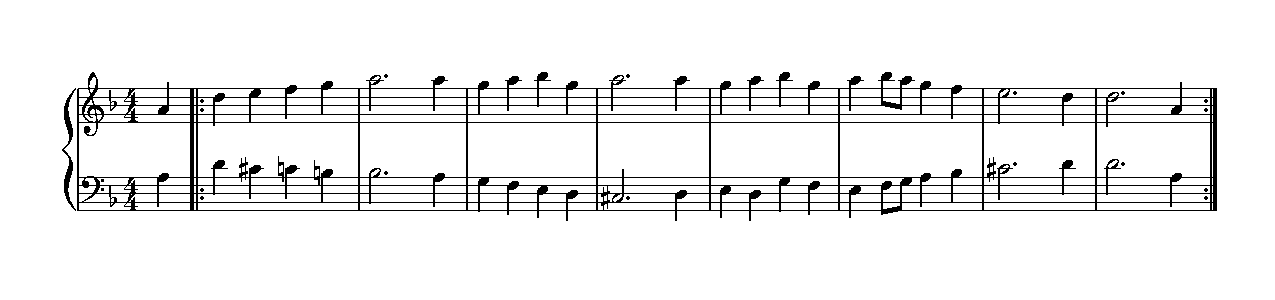
\includegraphics[scale=0.7]{code-pbind-start-stop-notation.pdf}}}
\caption{\texttt{Pbind} contraponto com uma melodia de Tchaikovsky}
\label{fig:counterpoint}
\end{figure}

Primeiro, repare no uso de variáveis. Uma delas, \texttt{minhasDurs}, é uma variável local. Dá pra saber que é uma variável local porque não começa com um til ($\sim$) e é declarada no início com a palavra-chave específica \texttt{\textbf{var}}. Esta variável contém um \texttt{Pseq} que será usado como \texttt{\textbackslash dur} em ambos os \texttt{Pbind}s. \texttt{minhasDurs} é necessária somente no momento de definir a partitura, então faz sentido usar uma variável local para isso (embora uma variável global funcionasse igualmente bem). As outras variáveis que você vê no exemplo são variáveis globais---uma vez declaradas, são válidas em qualquer lugar nos seus patches de SuperCollider.

Segundo, repare na separação ente partitura e tocadores, como discutimos anteriormente. Quando os \texttt{Pbind}s são definidos, eles não são tocados no mesmo momento---não há \texttt{.play} imediatamente depois de fechar os parênteses. Depois que você roda o primeiro bloco de código, tudo o que você tem são duas definições de \texttt{Pbind} armazenadas nas variáveis \texttt{$\sim$melodiaSuperior} e \texttt{$\sim$melodiaInferior}. Elas ainda não fazem som---são apenas partituras. A linha \texttt{$\sim$tocador1 = $\sim$melodiaSuperior.play} cria um \texttt{EventStreamPlayer} para cumprir a tarefa de tocar a melodia superior e a este tocador é dado o nome $\sim$tocador1. A mesma ideia vale para o $\sim$tocador2. Graças a isso, podemos falar com cada tocador e pedi-lo para parar, iniciar, retomar, etc.

Mesmo correndo o risco de sermos chatos, vamos reiterar uma última vez:
\begin{itemize}
\item Um \texttt{Pbind} é só uma receita para fazer som, como uma partitura musical;
\item Quando você chama a mensagem \texttt{play} em um \texttt{Pbind}, um objeto \texttt{EventStreamPlayer} é criado;
\item Se você armazena este \texttt{EventStreamPlayer} em uma variável, você pode acessá-lo mais tarde para usar comandos como \texttt{stop} e \texttt{resume}.
\end{itemize} 

% PART III
\newpage
\part{MAIS DETALHES SOBRE A LINGUAGEM}
\section{Objects, classes, messages, arguments}

SuperCollider is an Object-Oriented programming language, like Java or C++. It is beyond the scope of this tutorial to explain what this means, so we'll let you search that on the web if you are curious. Here we'll just explain a few basic concepts you need to know to better understand this new language you are learning.

Everything in SuperCollider is an \emph{object}. Even simple numbers are objects in SC. Different objects behave in different ways and hold different kinds of information. You can request some info or action from an object by sending it a \emph{message}. When you write something like \texttt{2.squared}, the message \texttt{squared} is being sent to the receiver object \texttt{2}. The dot between them makes the connection. Messages are also called \emph{methods}, by the way.

Objects are specified hierarchically in \emph{classes}. SuperCollider comes with a huge collection of pre-defined classes, each with their own set of methods.

Here's a good way to understand this. Let's imagine there is an abstract class of objects called \texttt{Animal}. The Animal class defines a few general methods (messages) common to all animals. Methods like \texttt{age}, \texttt{weight}, \texttt{picture} could be used to get information about the animal. Methods like \texttt{move}, \texttt{eat}, \texttt{sleep} would make the animal perform a specific action. Then we could have two subclasses of Animal: one called \texttt{Pet}, another called \texttt{Wild}. Each one of these subclasses could have even more subclasses derived from them (like \texttt{Dog} and \texttt{Cat} derived from \texttt{Pet}). Subclasses inherit all methods from their parent classes, and implement new methods of their own to add specialized features. For example, both Dog and Cat objects would happily respond to the \texttt{.eat} message, inherited from the Animal class. \texttt{Dog.name} and \texttt{Cat.name} would return the name of the pet: this method is common to all objects derived from Pet.  \texttt{Dog} has a \texttt{bark} method, so you can call \texttt{Dog.bark} and it will know what to do. \texttt{Cat.bark} would throw you an error message: \texttt{ERROR: Message 'bark' not understood.}

In all these hypothetical examples, the words beginning with a capital letter are \emph{classes} which represent \emph{objects}. The lowercase words after the dot are \emph{messages} (or \emph{methods}) being sent to those objects. Sending a message to an object always returns some kind of information. Finally, messages sometimes accept (or even require) \emph{arguments}. Arguments are the things that come inside parentheses right after a message. In \texttt{Cat.eat("sardines", 2)}, the message \texttt{eat} is being sent to \texttt{Cat} with some very specific information: what to eat, and quantity. Sometimes you will see arguments declared explicitly inside the parentheses (keywords ending with a colon). This is often handy to remind the reader what the argument refers to. \texttt{Dog.bark(volume: 10)} is more self-explanatory than just \texttt{Dog.bark(10)}.

\begin{figure}[h]
\centerline{\framebox{
	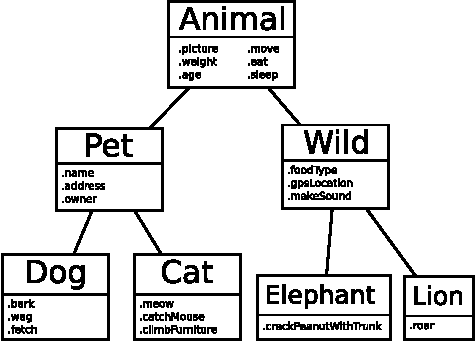
\includegraphics[scale=0.9]{fig-animal-class-chart.pdf}}}
\caption{Hypothetical class hierarchy.}
\label{fig:animal-class-chart}
\end{figure}

OK---enough of this quick and dirty explanation of object-oriented programming. Let's try some examples that you can actually run in SuperCollider. Run one line after the other and see if you can identify the message, the receiver object, and the arguments (if any). The basic structure is \texttt{Receiver.message(arguments)} Answers at the end of this document.\endnote{First line: the Array \texttt{[1, 2, 3, "wow"]} is the receiving object; \texttt{reverse} is the message. Second line: the String "hello" is the receiving object; \texttt{dup} is the message; \texttt{4} is the argument to \texttt{dup}. Third line: 3.1415 is the receiving object; \texttt{round} is the message; \texttt{0.1} is the argument to \texttt{round}. Fourth line: \texttt{100} is the receiver object, \texttt{rand} is the message. Last line: \texttt{100.0} is the receiver of the message \texttt{rand}, the result of which is a random number between 0 and 100. That number becomes the receiver of the message \texttt{round} with argument \texttt{0.01}, so that the random number is rounded to two decimal cases. Then this result becomes the receiving object of the message \texttt{dup} with argument \texttt{4}, which creates a list with four duplicates of that number.}

 
\begin{lstlisting}[style=SuperCollider-IDE, basicstyle=\scttfamily\footnotesize]
[1, 2, 3, "wow"].reverse;
"hello".dup(4); 
3.1415.round(0.1); // note that the first dot is the decimal case of 3.1415
100.rand; // evaluate this line several times
// Chaining messages is fun:
100.0.rand.round(0.01).dup(4);
\end{lstlisting}
\section{Receiver notation, functional notation}

There is more than one way of writing your expressions in SuperCollider. The one we just saw above is called \emph{receiver notation}: \texttt{100.rand}, where the dot connects the Object (\texttt{100}) to the message (\texttt{rand}). Alternatively, the exact same thing can also be written like this: \texttt{rand(100)}. This one is called \emph{functional notation}.

You can use either way of writing. Here's how this works when a message takes two or more arguments.

 
\begin{lstlisting}[style=SuperCollider-IDE, basicstyle=\scttfamily\footnotesize]
5.dup(20);  // receiver notation
dup(5, 20); // same thing in functional notation

3.1415.round(0.1); // receiver notation
round(3.1415, 0.1); // functional notation
\end{lstlisting}
 

In the examples above, you might read \texttt{dup(5, 20)} as ``duplicate the number 5 twenty times,'' and \texttt{round(3.1415, 0.1)} as ``round the number 3.1415 to one decimal case.'' Conversely, the receiver notation versions could be read as ``Number 5, duplicate yourself twenty times!'' (for \texttt{5.dup(20)}) and ``Number 3.1415, round yourself to one decimal case!'' (for \texttt{3.1415.round(0.1)}).

In short: \texttt{Receiver.message(argument)} is equivalent to \texttt{message(Receiver, argument)}.

Choosing one writing style over another is a matter of personal preference and convention. Sometimes one method can be clearer than the other. Whatever style you end up preferring (and it's fine to mix them), the important thing is to be consistent. One convention that is widespread among SuperCollider users is that classes (words that begin with uppercase letters) are almost always written as \texttt{Receiver.message(argument)}. For example, you will always see \texttt{SinOsc.ar(440)}, but you will almost never see \texttt{ar(SinOsc, 440)}, even though both are correct.

Exercise: rewrite the following statement using functional notation only:

\texttt{100.0.rand.round(0.01).dup(4);} 

Solution at the end.\endnote{Rewriting using functional notation only: \texttt{dup(round(rand(100.0), 0.01), 4);}}
\section{Nesting}
\label{sec:nesting}

The solution to the last exercise has led you to nest things one inside the other. David Cottle has an excellent explanation of nesting in the SuperCollider book, so we will just quote it here.\footnote{Cottle, D. ``Beginner's Tutorial.'' The SuperCollider Book, MIT Press, 2011, pp. 8-9.}

\begin{quotation}
\textit{To further clarify the idea of nesting, consider a hypothetical example in which SC will make you lunch. To do so, you might use a} \texttt{serve} message. \textit{The arguments might be salad, main course, and dessert. But just saying} \texttt{serve(lettuce, fish, banana)} \textit{may not give you the results you want. So to be safe you could clarify those arguments, replacing each with a nested message and argument.}
\end{quotation}

\texttt{serve(toss(lettuce, tomato, cheese), bake(fish, 400, 20), mix(banana, icecream))
}
\begin{quotation}
\textit{SC would then serve not just lettuce, fish, and banana, but a tossed salad with lettuce, tomato, and cheese; a baked fish; and a banana sundae. These inner commands can be further clarified by nesting a message(arg) for each ingredient: lettuce, tomato, cheese, and so on. Each internal message produces a result that is in turn used as an argument by the outer message.}
\end{quotation}

\begin{lstlisting}[style=SuperCollider-IDE, basicstyle=\scttfamily\footnotesize, label=code-dinner]
// Pseudo-code to make dinner: 
serve(
	toss(
		wash(lettuce, water, 10),
		dice(tomato, small),
		sprinkle(choose([blue, feta, gouda]))
	),
	bake(catch(lagoon, hook, bamboo), 400, 20),
	mix(
		slice(peel(banana), 20),
		cook(mix(milk, sugar, starch), 200, 10)
	)
);
\end{lstlisting}

\begin{quotation}
\textit{When the nesting has several levels, we can use new lines and indents for clarity. Some messages and arguments are left on one line, some are spread out with one argument per line---whichever is clearer. Each indent level should indicate a level of nesting. (Note that you can have any amount of white space---new lines, tabs, or spaces---between bits of code.)}

[In the dinner example]\textit{ the lunch program is now told to wash the lettuce in water for 10 minutes and to dice the tomato into small pieces before tossing them into the salad bowl and sprinkling them with cheese. You've also specified where to catch the fish and to bake it at 400 degrees for 20 minutes before serving, and so on.}

\textit{To ``read'' this style of code you start from the innermost nested message and move out to each successive layer. Here is an example aligned to show how the innermost message is nested inside the outer messages.}
\end{quotation}

%\lstinputlisting[style=SuperCollider-IDE, basicstyle=\scttfamily\footnotesize]{code-nesting.scd}

\begin{lstlisting}[style=SuperCollider-IDE, basicstyle=\scttfamily\footnotesize]
                exprand(1.0, 1000.0);
           dup({exprand(1.0, 1000.0)}, 100);
      sort(dup({exprand(1.0, 1000.0)}, 100));
round(sort(dup({exprand(1.0, 1000.0)}, 100)), 0.01);
\end{lstlisting}

The code below is another example of nesting. Answer the questions that follow. You don't have to explain what the numbers are doing---the task is simply to identify the arguments in each layer of nesting. (Example and exercise questions also borrowed and slightly adapted from Cottle's tutorial.)

 
%\lstinputlisting[style=SuperCollider-IDE, basicstyle=\scttfamily\footnotesize, label=code-nested-music]{code-nested-music.scd}

\begin{lstlisting}[style=SuperCollider-IDE, basicstyle=\scttfamily\footnotesize]
// Nesting and proper indentation
(
{
	CombN.ar(
		SinOsc.ar(
			midicps(
				LFNoise1.ar(3, 24,
					LFSaw.ar([5, 5.123], 0, 3, 80)
				)
			),
			0, 0.4
		),
		1, 0.3, 2)
}.play;
)
\end{lstlisting}

\begin{enumerate}[a)]
\item What number is the second argument for \texttt{LFNoise1.ar}?
\item What is the first argument for \texttt{LFSaw.ar}?
\item What is the third argument for \texttt{LFNoise1.ar}?
\item How many arguments are in \texttt{midicps}?
\item What is the third argument for \texttt{SinOsc.ar}?
\item What are the second and third arguments for \texttt{CombN.ar}?
\end{enumerate}


 
See the end of this document for the answers.\endnote{ Answers: 
\begin{enumerate}[a)]
\item 24
\item $\left[5, 5.123\right]$ [both numbers and brackets)
\item Entire \texttt{LFSaw} line
\item Only one
\item 0.4
\item 1 and 0.3
\end{enumerate}
 }

\medskip
 
\bigskip
\todo[inline, color=green!40]{ 
TIP: If for whatever reason your code has lost proper indentation, simply select all of it and go to menu Edit$\rightarrow$Autoindent Line or Region, and it will be fixed.
}
\bigskip
\section{Fechamentos}

Há quatro tipos de fechamento: \texttt{(parênteses)}, \texttt{[colchetes]}, \texttt{\{chaves\}} e \texttt{"aspas duplas"}.

Cada um que você abre, deve ser fechado mais adiante. Isso é chamado "balancear", ou seja, manter devida correspondência entre os pares de fechamento em todo o seu código.

O IDE do SuperCollider automaticamente indica o fechamento de parênteses (também de colchetes e chaves) quando você fecha um par--- eles são destacados em vermelho. Se você clicar um parêntese que não tem um par de abertura/fechamento, você verá uma seleção em vermelho escuro indicando que algo está faltando. O balanceamento é uma maneira rápida de selecionar uma grande seção de código para ser executado, deletado ou para operações de copiar/colar. Você pode fazer um clique duplo em um parêntese de abertura ou fechamento para selecionar tudo o que está contido neles (o mesmo vale para colchetes e chaves).

\subsection{Aspas duplas}

Aspas duplas são usadas para definir uma sequência de caracteres (incluindo espaços) como uma coisa única. Estas são chamadas Strings ("cadeias"). Aspas simples criam Símbolos ("Symbols"), que são ligeiramente diferentes de Strings. Símbolos também podem ser criados com uma barra invertida imediatamente antes do texto. Portanto, \texttt{'queSimbolo'} and \texttt{\textbackslash queSimbolo} são equivalentes.

\begin{lstlisting}[style=SuperCollider-IDE, basicstyle=\scttfamily\footnotesize]
"Isto aqui é uma string";
'simboloLegalDemais';
\end{lstlisting}

\subsection{Parênteses}

Parênteses podem ser usados para:

\begin{itemize}
\item englobar listas de argumentos: \texttt{rrand(0, 10);}
\item forçar precedência: \texttt{5 + (10 * 4);}
\item criar blocos de código (múltiplas linhas de código para serem rodadas simultaneamente).
\end{itemize} 

\subsection{Colchetes}

Colchetes definem uma coleção de itens, como \texttt{[1, 2, 3, 4, "oi"]}. Estas são normalmente chamadas Arrays. Uma array pode conter qualquer coisa: números, strings, funções, Patterns, etc. Arrays entendem mensagens como \texttt{reverse} ("inverter"), \texttt{scramble} ("embaralhar"), \texttt{mirror} ("espelhar"), \texttt{choose} ("escolher"), para dar alguns exemplos. Você também pode fazer operações matemáticas em arrays.


\begin{lstlisting}[style=SuperCollider-IDE, basicstyle=\scttfamily\footnotesize]
[1, 2, 3, 4, "oi"].scramble;
[1, 2, 3, 4, "oi"].mirror;
[1, 2, 3, 4].reverse + 10;
// converter notas MIDI para frequências em Hz 
[60, 62, 64, 65, 67, 69, 71].midicps.round(0.1);
\end{lstlisting}

Mais sobre arrays em breve na seção \ref{sec:arrays}.

\subsection{Chaves}

Chaves definem funções. Funções encapsulam algum tipo de operação ou tarefa que será provavelmente reutilizada múltiplas vezes, possivelmente retornando diferentes resultados a cada vez. O exemplo abaixo é do The SuperCollider Book:

\begin{lstlisting}[style=SuperCollider-IDE, basicstyle=\scttfamily\footnotesize]
exprand(1, 1000.0);
{exprand(1, 1000.0)};
\end{lstlisting}

David Cottle nos explica passo a passo esse exemplo: \textit{"a primeira linha seleciona um número aleatório, que é mostrado na Post window. A segunda linha imprime um resultado bastante diferente: uma função. O que essa função faz? Ela seleciona um número aleatório. Como pode esta diferença afetar o código? Considere as linhas abaixo. A primeira escolhe um número aleatório e o duplica. A segunda executa  cinco vezes a função-seletora-de-números-aleatórios e coleta os resultados em uma array."}\footnote{Cottle, D. ``Beginner's Tutorial.'' The SuperCollider Book, MIT Press, 2011, p. 13.}

\begin{lstlisting}[style=SuperCollider-IDE, basicstyle=\scttfamily\footnotesize]
rand(1000.0).dup(5);  // seleciona um número e o duplica
{rand(1000.0)}.dup(5);  // duplica a função de selecionar um número 
{rand(1000.0)}.dup(5).round(0.1); // tudo o que foi feito acima, depois arredondando os valores
// um resultado semelhante a:
[rand(1000.0), rand(1000.0), rand(1000.0), rand(1000.0), rand(1000.0)]
\end{lstlisting}
 
Mais sobre funções em breve. Por ora, aqui está um resumo de todos os fechamentos possíveis:

\begin{description}
\item[Coleções] \texttt{[lista, de, itens]}
\item[Funções] \texttt{\{ operações a serem executadas \}}
\item[Strings] \texttt{"palavras entre aspas"}
\item[Símbolos] \texttt{‘aspasSimples’} ou precedidas de uma \texttt{\textbackslash barraInvertida}
\end{description}

\section{Condicionais: if/else e case}

Se estiver chovendo, eu levarei um guarda-chuva quando sair. Se estiver sol, levarei meus óculos escuros. Nossos dias estão repletos desse tipo de tomada de decisão. Em programação, estes são os momentos em que o seu código tem de testar alguma condição e realizar ações diferentes, dependendo do resultado do teste (verdadeiro ou falso). Há muitos tipos de estruturas condicionais. Vamos dar uma olhada em dois casos simples: \emph{if/else} (“se/senão”) e \emph{case} (“no caso de”).

A sintaxe de um if/else no SC é: \texttt{if(condition, \{true action\}, \{false action\})}. A condição é um teste booleano, ou seja, precisa retornar um \texttt{true} (“verdadeiro”) ou \texttt{false}(“falso”). Se o teste retorna verdadeiro, a primeira função roda. Se não, roda-se a segunda. Experimente:

\begin{lstlisting}[style=SuperCollider-IDE, basicstyle=\scttfamily\footnotesize]
// if / else 
if(100 > 50, { “muito verdadeiro”.postln }, { “muito falso“.postln });
\end{lstlisting}

A tabela abaixo, emprestada do The SuperCollider Book \footnote{Cottle, D. “Beginner's Tutorial.” The SuperCollider Book, MIT Press, 2011, p. 33}, apresenta alguns operadores booleanos comuns que podem ser usados.
Note a distinção entre um sinal de igual simples (\texttt{x = 10}) e o sinal de igual duplo (\texttt{x == 10}). O simples significa “\textit{atribua 10 à variável x},” ao passo que o duplo significa “\textit{é x igual a 10?}” Digite e rode alguns exemplos da coluna de verdadeiro ou falso e você verá parecerem os resultados \texttt{true} ou  \texttt{false} aparecerem na Post window.
 
\begin{center}
\begin{tabular}{llll}
\hline 
\textbf{Símbolo} & \textbf{Significado} & \textbf{Exemplo verdadeiro} & \textbf{Exemplo falso} \\ 
\hline 
\texttt{==} & igual a? & \texttt{10 == 10} & \texttt{10 == 99} \\ 
\hline 
\texttt{!=} & não é igual a? & \texttt{10 != 99} & \texttt{10 != 10} \\ 
\hline 
\texttt{>} & maior que? & \texttt{10 > 5} & \texttt{10 > 99} \\ 
\hline 
\texttt{<} & menor que? & \texttt{10 < 99} & \texttt{10 < 5} \\ 
\hline 
\texttt{>=} & maior ou igual a?  & \texttt{10 >= 10}, \texttt{10 >= 3} & \texttt{10 >= 99} \\ 
\hline 
\texttt{<=} & menor ou igual a? & \texttt{10 <= 99}, \texttt{10 <= 10} & \texttt{10 <= 9} \\ 
\hline 
\texttt{odd} & é ímpar? & \texttt{15.odd} & \texttt{16.odd} \\ 
\hline 
\texttt{even} & é par? & \texttt{22.even} & \texttt{21.even} \\ 
\hline 
\texttt{isInteger} & é um número inteiro? & \texttt{3.isInteger} & \texttt{3.1415.isInteger} \\ 
\hline 
\texttt{isFloat} & é um número decimal? & \texttt{3.1415.isFloat} & \texttt{3.isFloat} \\ 
\hline 
\texttt{and} & ambas as condições & \texttt{11.odd.and(12.even)} & \texttt{11.odd.and(13.even)} \\ 
\hline 
\texttt{or} & uma das condições & \texttt{or(1.odd, 1.even)} & \texttt{or(2.odd, 1.even)} \\ 
\hline 
\end{tabular} 
\end{center}
 

As últimas duas linhas (\texttt{and}, \texttt{or}) mostram como escrever as expressões mais longas tanto em notação de objeto recebedor quanto em notação funcional.

Outra estrutura útil é \texttt{case}. Ela funciona definindo pares de funções a serem executadas na ordem até que um dos testes retorne verdadeiro:

\texttt{case}

\texttt{\{teste1\} \{ação1\}}

\texttt{\{teste2\} \{ação2\}}

\texttt{\{teste3\} \{ação3\}}

\dots

\texttt{\{testeN\} \{açãoN\}};

A expressão dentro de cada teste tem de retornar ou \texttt{true} ou \texttt{false}. Se o teste1 retorna falso, o programa ignora a ação1 e segue para o teste2. Se for um falso, ação2 também é ignorada e seguimos para o teste3. Se este for verdadeiro, então a ação3 é executada e o \texttt{case} para (mais nenhum teste ou ação é executado). Note que não há vírgulas entre as funções. Simplesmente use um ponto-e-vírgula no fim para marcar o final do enunciado \texttt{case}.

 
\begin{lstlisting}[style=SuperCollider-IDE, basicstyle=\scttfamily\footnotesize]
// case
(
~num = -2;

case
{~num == 0} {“UAU”.postln}
{~num == 1} {“UM!”.postln}
{~num < 0} {“número negativo!”.postln}
{true} {“em último caso“.postln};
)
\end{lstlisting}
 
Tente modificar o código acima para obter todos os resultados possíveis. Perceba o truque útil (e opcional) na última linha de \texttt{case} no exemplo acima: como \texttt{true} sempre retorna verdadeiro, pode-se definir uma ação para acontecer “em último caso” que vai sempre ocorrer, mesmo no caso de todas as condições anteriores serem falsas.

Para saber mais, verifique o arquivo de ajuda de Control Structures (“Estruturas de Controle”).

\section{Funções}
\label{sec:functions}

Quando você se vê fazendo a mesma tarefa diversas vezes, talvez seja um bom momento para criar uma função reutilizável. Uma função, como você aprendeu na seção de Fechamentos, é algo escrito entre chaves. David Touretzky introduz a ideia de função da seguinte forma: "pense na função como uma caixa através da qual os dados passam. Essa função opera sobre os dados de alguma forma e o resultado é o que passa para fora." \footnote{Touretzky, David. COMMON LISP: A Gentle Introduction to Symbolic Computation. The Benjamin/Cummings Publishing Company, Inc, 1990, p. 1. Este é o livro que inspirou o título original em inglês deste tutorial.}

\begin{figure}[h]
\centerline{\framebox{
	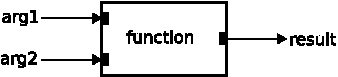
\includegraphics[scale=0.9]{fig-function-box.pdf}}}
\caption{Ideia geral de uma função.}
\label{fig:function-box}
\end{figure}

A primeira linha no exemplo abaixo define a função, atribuindo-a à variável \texttt{f}. A segunda linha coloca a função para trabalhar.

 
\begin{lstlisting}[style=SuperCollider-IDE, basicstyle=\scttfamily\footnotesize]
f = { 2 + 2 }; // define a função
f.value; // colocar a função para trabalhar
\end{lstlisting}
 
A função acima não é terrivelmente útil, pois apenas sabe fazer uma única coisa (somar 2 e 2). Normalmente você vai querer definir funções que podem dar diferentes resultados dependendo dos argumentos de entrada que você forneça. Nós usamos a palavra-chave \texttt{arg} para especificar as entradas que uma função pode aceitar. O exemplo abaixo é mais parecido com o desenho da figura \ref{fig:function-box}.
 
\begin{lstlisting}[style=SuperCollider-IDE, basicstyle=\scttfamily\footnotesize]
f = {arg a, b; ["a mais b", a+b, "a vezes b", a*b].postln}; // define função
f.value(3, 7); // agora você pode dois números quaisquer como argumentos para a função
f.value(10, 14);

// Compare:
~sillyRand = rrand(0, 10); // não é uma função
~sillyRand.value; // execute diversas vezes
~sillyRand2 = {rrand(0, 10)}; // é uma função
~sillyRand2.value; // execute diversas vezes
\end{lstlisting}
 
Como um último exemplo, aqui está uma função muito útil.
 
\begin{lstlisting}[style=SuperCollider-IDE, basicstyle=\scttfamily\footnotesize]
// Use esta função para decidir como passar seus dias de verão

(
~oQueFazer = { 
var hoje, nomeDoDia, acoes;
	hoje = Date.getDate.dayOfWeek;
	nomeDoDia = 
	case
	{hoje==0} {"Domingo"}
	{hoje==1} {"Segunda"}
	{hoje==2} {"Terça"}
	{hoje==3} {"Quarta"}
	{hoje==4} {"Quinta"}
	{hoje==5} {"Sexta"}
	{hoje==6} {"Sábado"};
	acoes = ["jogar bumerangue", "queda de braço", "subir escadas", "jogar xadrez", "hóquei subaquático", "atirar ervilhas", "longa soneca"];
	"Ah, " ++ nomeDoDia ++ "...! " ++ "Que ótimo dia para " ++ acoes.choose;
};
)

// Execute pela manhã
~oQueFazer.value;
\end{lstlisting}

\bigskip
\todo[inline, color=green!40]{ DICA: Outra notação comum para declarar argumentos no início de uma Função é: \texttt{f = \{|a, b| a + b\}}. Isso é equivalente a \texttt{f = \{arg a, b; a + b\}}} 


\section{Divirta-se com Arrays}
\label{sec:arrays}

Arrays [N.T.: em computação, o termo "array" pode ser traduzido como "vetor", mas é comum mantê-lo no original] são o tipo mais comum de coleção no SuperCollider. Toda vez que você escreve uma coleção de itens entre colchetes, como \texttt{[0, 1, 2]}, cria uma instância da classe \texttt{Array}. Frequentemente, você se verá manipulando arrays de diversas formas. Aqui está uma pequena seleção de métodos interessantes que arrays entendem:

 
\begin{lstlisting}[style=SuperCollider-IDE, basicstyle=\scttfamily\footnotesize]
// Criar uma array
a = [10, 11, 12, 13, 14, 15, 16, 17];

a.reverse;  // inverter
a.scramble; // embaralhar
a.choose;  // escolher um elemento ao acaso
a.size;	  // retorna o tamanho da array
a.at(0);   // recupera um item na posição especificada
a[0]	;  // o mesmo que acima
a.wrapAt(9); // recupera item na posição especificada, relendo do início se > a.size
["wow", 99] ++ a; // concatena duas arrays em uma nova
a ++ \oi;  // um Símbolo é entendido como um único caracter
a ++ 'oi'; // o mesmo que acima
a ++ "oi"; // uma cadeia ("String") é entendida como uma coleção de caracteres
a.add(44);    // cria uma nova array adicionando o novo elemento ao final
a.insert(5, "uau"); // insere "uau" na posição 5, empurra itens seguintes para a frente (retorna uma nova array)
a; // rode isso e veja que nenhuma das operações acima mudou a array original
a.put(2, "oops"); // colocar "oops" no índice 2 (destrutivo; volte a rodar a linha acima para verificar)
a.permute(3); // permutar: item na posição 3 vai para a posição zero, e vice-versa
a.mirror;  // faz um palíndromo
a.powerset; // retorna todas as possíveis combinações dos elementos da array
\end{lstlisting}
 

Você pode fazer contas com arrays:

 
\begin{lstlisting}[style=SuperCollider-IDE, basicstyle=\scttfamily\footnotesize]
[1, 2, 3, 4, 5] + 10;
[1, 2, 3, 4, 5] * 10;
([1, 2, 3, 4, 5] / 7).round(0.01); // note o uso de parênteses para precedência
x = 11; y = 12; // experimente algumas variáveis
[x, y, 9] * 100;
// mas garanta que você só faça contas com números de verdade
[1, 2, 3, 4, "oops", 11] + 10; // resultado estranho
\end{lstlisting}
 

\subsection{Creating new Arrays}

Aqui há algumas maneiras de usar a classe \texttt{Array} para criar novas coleções:

\begin{lstlisting}[style=SuperCollider-IDE, basicstyle=\scttfamily\footnotesize]
// Progressão aritmética (definindo tamanho, início e passo da progressão)
Array.series(size: 6, start: 10, step: 3);
// Progressão geométrica (definindo tamanho, início e razão da progressão)
Array.geom(size: 10, start: 1, grow: 2);
// Compare as duas:
Array.series(7, 100, -10); // 7 itens; começando em 100, passo de -10
Array.geom(7, 100, 0.9); // 7 itens; começando em 100; multiplicar por 0.9 a cada vez
// Conheça o método .fill
Array.fill(10, "igual");
// Compare:
Array.fill(10, rrand(1, 10)); 
Array.fill(10, {rrand(1, 10)}); // a função é reexecutada 10 vezes
// A função definida como segundo arg do método .fill pode receber um contador como argumento padrão.
// O nome do argumento pode ser o que você quiser.
Array.fill(10, {arg contador; contador * 10});
// Por exemplo, gerando uma lista de frequências harmônicas:
Array.fill(10, {arg uau; uau+1 * 440}); 
// O método .newClear
a = Array.newClear(7); // cria uma array vazia do tamanho desejado
a[3] = "uau"; // mesmo que a.put(3, "uau")
\end{lstlisting}


\subsection{Aquele ponto de exclamação esquisito}

É só uma questão de tempo até que você veja algo como \texttt{30!4} no código de alguém. Essa notação abreviada simplesmente cria uma array contendo o mesmo item um determinado número de vezes:

 
\begin{lstlisting}[style=SuperCollider-IDE, basicstyle=\scttfamily\footnotesize]
// Notação abreviada:
30!4;
"alô" ! 10;
// Dá o mesmo resultado que o seguinte:
30.dup(4);
"alô".dup(10);
// ou
Array.fill(4, 30);
Array.fill(10, "alô");
\end{lstlisting}
 

\subsection{Os dois pontos entre parênteses}

Aqui está mais uma sintaxe abreviada muito usada para criar arrays.

 
\begin{lstlisting}[style=SuperCollider-IDE, basicstyle=\scttfamily\footnotesize]
// Que diabo é isso?
(50..79);
// É um atalho para gerar uma array com uma progressão numérica aritmética.
// O atalho acima tem o mesmo resultado que:
series(50, 51, 79);
// ou
Array.series(30, 50, 1);
// Para um passo (razão) diferente de 1, você pode fazer o seguinte:
(50, 53 .. 79); // de 3 em 3
// Mesmo resultado que:
series(50, 53, 79);
Array.series(10, 50, 3);
\end{lstlisting}

Note que cada comando implica um jeito de pensar ligeiramente diferente. O \texttt{(50..79)} permite que você pense assim: "\emph{me dê uma array de 50 a 79}." Você não precisa necessariamente pensar a quantidade de itens que a lista vai conter. Por outro lado, \texttt{Array.series} permite pensar: "\emph{me dê uma array com 30 itens no total, começando a partir do 50}." Você não precisa necessariamente pensar qual será o último número da série.

Também note que o atalho usa parênteses, não colchetes. A array resultante, naturalmente, virá entre colchetes.
\subsection{Como "fazer" um Array}

Muitas vezes você vai precisar realizar alguma operação com cada um dos itens de uma coleção. Você pode usar o método \texttt{do} ("faça") para isso:


\begin{lstlisting}[style=SuperCollider-IDE, basicstyle=\scttfamily\footnotesize]
~minhasFreqs = Array.fill(10, {rrand(440, 880)});

//Agora vamos fazer uma ação simples com cada um dos itens da lista:
~minhasFreqs.do({arg item, contador; ("Item " ++ contador ++ " é " ++ item ++ " Hz. A nota MIDI mais próxima é " ++ item.cpsmidi.round).postln});

// Se você não precisa do contador, use apenas um argumento:
~minhasFreqs.do({arg item; item.squared.postln});

// Claro que algo simples como o exemplo anterior poderia ser feito assim:
~minhasFreqs.squared;
\end{lstlisting}
 

Em resumo: quando você processa uma array com "do", você fornece uma função. A mensagem \texttt{"do"} vai cuidar de executar a função uma vez para cada item constante da array. A função pode receber dois argumentos por definição: o item da vez propriamente dito, e um contador que vai registrando o número de iterações já realizadas. Os nomes destes argumentos podem ser o que você quiser, mas estarão sempre nesta ordem: item, contador.

Veja também o método \texttt{collect}, que é muito similar ao \texttt{do}, mas retorna uma nova coleção com todos os resultados intermediários.

\section{Obtendo Ajuda}

Aprenda a usar bem os arquivos da Ajuda (“Help”). Muitas vezes, ao final de cada página da Ajuda, há exemplos úteis.  Role a página para baixo para conferi-los, mesmo que (ou especialmente se) você não entendeu completamente as explicações do texto. Você pode rodar os exemplos diretamente do browser da Ajuda ou você pode copiar e colar o código em uma nova janela para brincar com ele. 

Selecione qualquer classe ou método válidos no seu código de SuperCollider (um duplo-clique na palavra irá selecioná-la) e aperte [ctrl+D] para abrir o arquivo de Help correspondente. Se você selecionar o nome de uma classe (por exemplo, \texttt{MouseX}), você será direcionado para o arquivo de Ajuda da classe. Se você selecionar um método (por exemplo, peça ajuda do método \texttt{scramble}. \footnote{Atenção: O SuperCollider vai mostrar em azul qualquer palavra que começa com uma letra maiúscula. Isso significa que a cor azul \emph{não garante} que a palavra esteja livre de erros: por exemplo, se você digitar Sinosc (com o “o” minúsculo incorreto), ainda assim a palavra aparece em azul.}

Outras maneiras de explorar os arquivos de Ajuda da IDE do SuperCollider são os links “Browse” (“Navegar”) e “Search” (“Pesquisar”). Use o Browse para navegar os arquivos por categorias e o Search para pesquisar palavras em todos os arquivos de Ajuda.
Nota importante sobre o Browser de Ajuda na IDE do SuperCollider:

\begin{itemize}
\item Use o campo superior direito (onde se lê “Find…”) para procurar palavras específicas \emph{dentro do arquivo de Help que está aberto} (como você usaria um “find” para localizar algo em um website);
\item Use o link “Search” (à direita de “Browse”) para procurar texto \emph{em todos os arquivos de Ajuda}.
\end{itemize}

Quando você abrir o primeiro parênteses para adicionar argumentos para um método específico, o SC mostra uma pequena “dica de ajuda” para mostrar quais são os argumentos esperados. Por exemplo, digite o início de uma linha que você vê na figura \ref{fig:tooltip}. Logo depois de abrir o primeiro parênteses, a dica mostra que os argumentos para um \texttt{SinOsc.ar} são \texttt{freq}, \texttt{phase}, \texttt{mul} e \texttt{add}. Também aparecem os valores padrão. Esta é exatamente a mesma informação que você obteria no arquivo de Ajuda do \texttt{SinOsc}. Se a dica de ajuda desapareceu, você pode trazê-la de volta com [ctrl+Shift+Espaço].

\begin{figure}[h]
\centerline{\framebox{
	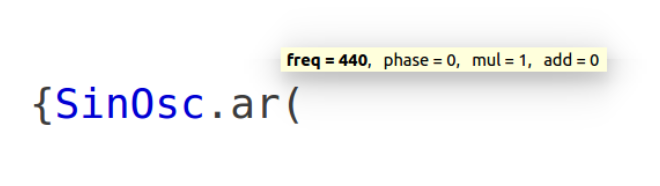
\includegraphics[scale=0.3]{fig-help-tooltip-crop.png}}}
\caption{Informação útil é mostrada conforme você vai digitando.}
\label{fig:tooltip}
\end{figure}

Outro atalho: se você quiser explicitamente nomear seus argumentos (como \texttt{SinOsc.ar(freq: 890)}), experimente apertar a tecla Tab logo depois de abrir os parênteses. O SC vai autocompletar para você com o nome do argumento correto, na ordem, à medida que você digita (aperte Tab depois da vírgula para os nomes dos argumentos subsequentes).

\bigskip
\todo[inline, color=green!40]{ 
DICA: Crie uma pasta com seus próprios “arquivos pessoais de ajuda”. Sempre que você descobrir um novo truque ou aprender um novo objeto, escreva um exemplo simples com explicações em suas próprias palavras e salve-o para o futuro. Isso pode ser útil daqui um mês ou um ano.

}
\bigskip

Os mesmos arquivos de Ajuda podem ser também encontrados onlin \url{http://doc.sccode.org/}.

% PART IV
\newpage
\part{SÍNTESE E PROCESSAMENTO SONORO}
Neste ponto, você já sabe bastante sobre o SuperCollider. A última parte deste tutorial apresentou para você detalhes minuciosos sobre a própria linguagem, de variáveis a fechamentos e muito mais. Você também aprendeu como criar \texttt{Pbind}s interessantes, usando vários membros da família Pattern.

Esta parte do tutorial vai (finalmente!) apresentar síntese e processamento sonoros com o SuperCollider. Começaremos com o tópico das Unit Generators ("Unidades Geradoras" ou "Geradores Unitários", que daqui em diante chamaremos UGens). \footnote{A maioria dos tutoriais começa diretamente com as UGens; nesta introdução ao SC, no entanto, escolhemos primeiro enfatizar a família Pattern (\texttt{Pbind} e seus amigos) para uma abordagem pedagógica diferente.}

\section{UGens}

Você já viu algumas Unidades Geradoras (UGens) em ação nas seções \ref{sec:first-sine} e \ref{sec:nesting}. O que é uma UGen? Uma unidade geradora é um objeto que gera sinais sonoros e sinais de controle. Estes sinais são sempre calculados no servidor. Há muitas classes de unidades geradoras, todas elas derivando da classe UGen. \texttt{SinOsc} e \texttt{LFNoise0} são exemplos de UGens. Para mais detalhes, veja os arquivos de Ajuda chamados "Unit Generators and Synths" e "Tour of UGens". 

Quando você tocou seus Pbinds num momento anterior deste tutorial, o som padrão era sempre o mesmo: um sintetizador simples semelhante a um piano. Este sintetizador é feito de uma combinação de unidades geradoras.\footnote{Como você usou \texttt{Pbind}s até aqui para fazer som no SuperCollider, pode ser tentador pensar: \textit{"Entendi, então o \texttt{Pbind} é uma Unidade Geradora!"} Não é o caso. \texttt{Pbind} não é uma Unidade Geradora---ela é apenas uma receita para fazer eventos musicais (partitura). \textit{"Então o \texttt{EventStreamPlayer}, a coisa que aparece quando eu chamo \texttt{play} em um \texttt{Pbind}, ISSO deve ser um UGen!"} A resposta ainda é não. O \texttt{EventStreamPlayer} é apenas o tocador, como um pianista, e o pianista não gera som. Continuando com esta metáfora limitada, o \emph{instrumento piano} é a coisa que realmente vibra e produz som. Está é uma analogia mais adequada para a UGen: não é a partitura, não é o tocador: é o instrumento. Quando você fez música com \texttt{Pbind}s antes, o SC criava um \texttt{EventStreamPlayer} para tocar sua partitura com seu sintetizador de piano embutido. Você não tinha de se preocupar em criar o piano ou algo assim---o SuperCollider fez todo o trabalho nos bastidores para você. Aquele sintetizador de piano escondido é feito de uma combinação de umas poucas Unidades Geradoras.} Você aprenderá como combinar unidades geradoras para criar todo tipo de instrumentos com sons sintéticos e processados. O último exemplo parte da nossa primeira senoide para criar um instrumento eletrônico que você pode tocar ao vivo com o mouse.

\subsection{Controle do Mouse: Theremin instantâneo}

Aqui está um sintetizador simples que você pode tocar em tempo real. É uma simulação do Theremin, um dos mais antigos instrumentos eletrônicos:

\begin{lstlisting}[style=SuperCollider-IDE, basicstyle=\scttfamily\footnotesize]
{SinOsc.ar(freq: MouseX.kr(300, 2500), mul: MouseY.kr(0, 1))}.play;
\end{lstlisting}

Se você não sabe o que é um Theremim, por favor pare tudo agora e procure por "Clara Rockmore Theremin" no YouTube. Depois volte aqui e tente tocar o Canto do cisne com o seu Theremin de SuperCollider.

\texttt{SinOsc}, \texttt{MouseX} e \texttt{MouseY} são UGens. \texttt{SinOsc} está gerando o som da onda senoidal. Os outros dois estão captando o movimento do seu cursor na tela (X para o movimento horizontal e Y para o movimento vertical) e usando os números para alimentar os valores de frequência e amplitude da senoide. Muito simples e muito divertido.

\subsection{Dente-de-serra e onda quadrada; gráfico e osciloscópio}

O Theremin acima usou um oscilador senoidal. Há outras formas de onda que você pode usar para fazer som. Rode as linhas abaixo---elas usam o conveniente método \texttt{plot} ("gráfico")---para olhar a forma do\texttt{SinOsc} e compará-lo com \texttt{Saw} e \texttt{Pulse}. As linhas abaixo não produzem som---elas apenas permitem que você visualize uma fotografia da forma de onda.

\begin{lstlisting}[style=SuperCollider-IDE, basicstyle=\scttfamily\footnotesize]
{ SinOsc.ar }.plot; // onda senoidal
{ Saw.ar }.plot; // onda dente-de-serra
{ Pulse.ar }.plot; // onda quadrada
\end{lstlisting}

Agora reescreva sua linha de Theremin, substituindo \texttt{SinOsc} por \texttt{Saw}, depois por \texttt{Pulse}. Escute como eles soam diferente. Finalmente, experimente \texttt{.scope} em vez de \texttt{.play} no seu código de Theremin e você poderá ver uma representação da forma de onda em tempo real (abrirá uma janela "Stethoscope", que na realidade é um osciloscópio).

\section{Audio rate, control rate}

É bastante fácil identificar uma UGen em um código de SuperCollider: elas são quase sempre seguidas pelas mensagens \texttt{.ar} ou \texttt{.kr}. Estas letras querem dizer Audio Rate ("taxa de áudio") e Control Rate ("taxa de controle"). Vamos ver o que isso significa.

Do arquivo de ajuda "Unit Generators and Synths" ("Unidades geradoras e Sintetizadores"): 

\begin{quotation}
Uma unidade geradora é criada ao se enviar uma mensagem \texttt{ar} ou \texttt{kr} para um objeto da classe da respectiva unidade geradora. A mensagem \texttt{ar} cria uma UGen que é executada na velocidade da taxa de áudio. A mensagem \texttt{kr} cria uma UGen executada na velocidade da taxa de controle. UGens de controle são usados para sinais de controle de baixa frequência ou que mudem lentamente. UGens de controle produzem uma única amostra por ciclo de controle e, por isso, utilizam menos poder de processamento que UGens de áudio. \footnote{\url{http://doc.sccode.org/Guides/UGens-and-Synths.html}}
\end{quotation}

Em outras palavras: quando você escreve \texttt{SinOsc.ar}, você está mandando a mensagem "taxa de áudio" para a UGen  \texttt{SinOsc} UGen. Assumindo que seu computador esteja rodando na taxa de amostragem comum de 44100 Hz, este oscilador senoidal vai gerar 44100 amostras por segundo para serem enviadas ao alto-falante. Então escutamos uma onda senoidal.

Reflita por um momento sobre o que você acabou de ler: quando você manda a mensagem \texttt{ar} para uma UGen, você esta pedindo que que ela gere \emph{quarenta e quatro mil e cem} números por segundo. Isso é um monte de números. Você escreve \texttt{\{SinOsc.ar\}.play} na linguagem e a linguagem comunica seu pedido ao servidor. O verdadeiro trabalho de gerar todas estas amostras é feito pelo servidor, o "motor sonoro" do SuperCollider.

Agora, quando você usa \texttt{kr} em vez de \texttt{ar}, o trabalho tambem é feito pelo servidor, mas há algumas diferenças:
\begin{enumerate}
\item A quantidade de números gerados por segundo com \texttt{.kr} é muito menor. \texttt{\{SinOsc.ar\}.play} gera 44100 números por segundo, enquanto \texttt{\{SinOsc.kr\}.play} fornece um pouco menos de 700 números por segundo (se você tiver curiosidade, a quantidade exata é 44100 / 64, sendo que 64 é o chamado "período de controle".)
\item O sinal gerado com \texttt{kr} não vai para os alto-falantes. Em vez disso, é normalmente utilizado para controlar parâmetros de outros sinais---por exemplo, o \texttt{MouseX.kr} no seu theremim estava controlando a frequência de um \texttt{SinOsc}.

\end{enumerate} 

OK, então UGens são estes geradores de números incrivelmente velozes. Alguns destes números se tornam sinais sonoros; outros se tornam sinais de controle. Até aí, tudo bem. Mas que números são estes, afinal de contas? Grandes? Pequenos? Positivos? Negativos? Na verdade, eles são números bem pequenos, muitas vezes entre -1 e +1. Às vezes somente entre 0 e 1. Todos os UGens podem ser divididos em duas categorias, de acordo com a abrangência dos números que eles geram: UGens unipolares e UGens bipolares.

\begin{description}
\item[UGens unipolares] geram números entre 0 e 1.
\item[UGens bipolares] geram números entre -1 e +1.

\end{description}

\subsection{O método \texttt{poll}}

Examinar a saída de alguns UGens pode esclarecer isso. Não podemos esperar que o SuperCollider imprima milhares de números por segundo na Post window, mas podemos pedir que ele imprima alguns deles, apenas para termos uma ideia. Digite e rode as seguintes linhas, uma de cada vez (garanta que seu servidor esteja rodando), e observe a Post window: 

\begin{lstlisting}[style=SuperCollider-IDE, basicstyle=\scttfamily\footnotesize]
// apenas observe a Post window (sem som)
{SinOsc.kr(1).poll}.play;
// pressione ctrl+ponto final, então rode a próxima linha:
{LFPulse.kr(1).poll}.play;
\end{lstlisting}

Os exemplos não produzem som algum porque estamos usando \texttt{kr}---o resultado é um sinal de controle, então nada é enviado para os alto-falantes. O objetivo aqui é apenas observar a saída típica de um \texttt{SinOsc}. A mensagem \texttt{poll} pega 10 números por segundo da saída do \texttt{SinOsc} e as imprime na Post window. O argumento 1 é a frequência, que apenas quer dizer que a onda senoidal vai demorar um segundo para completar um ciclo inteiro. Baseado no que você observou, o \texttt{SinOsc} é unipolar ou bipolar? E o \texttt{LFPulse}?\endnote{\texttt{SinOsc} é bipolar porque dá saída a números entre 1- e +1. \texttt{LFPulse} é unipolar porque o âmbito da saída é 0-1 (de fato, o \texttt{LFPulse} em particular somente dá saída a zeros e uns, sem nada intermediário)}

Abaixe todo o volume antes de rodar a próxima linha, depois aumente-o devagar. Você deve ouvir cliques suaves.

\begin{lstlisting}[style=SuperCollider-IDE, basicstyle=\scttfamily\footnotesize]
{LFNoise0.ar(1).poll}.play;
\end{lstlisting}

Como mandamos para ele uma mensagem \texttt{ar}, este gerador de ruído de baixa frequência ("Low Frequency Noise") o gerador esta enviando 44100 amostras por segundo para a sua placa de som---é um sinal de áudio. Cada amostra é um número entre -1 e +1 (então é uma UGen bipolar). Com \texttt{poll} você está vendo somente dez deles por segundo. \texttt{LFNoise0.ar(1)} escolhe um novo número randômico a cada segundo. Tudo isto é feito pelo servidor.

Pare os clicks com [ctrl+.] e experimente mudar a frequência de \texttt{LFNoise0}. Tente números como 3, 5, 10 e depois mais altos. Observe os números produzidos e ouça os resultados.

\section{Argumentos de UGen}

Na maior parte do tempo você vai querer especificar argumentos para as UGens que você estiver usando. Você já viu isso: quando você escreve \texttt{\{SinOsc.ar(440)\}.play}, o número \texttt{440} é um argumento para o \texttt{SinOsc.ar}; ele especifica a frequência que você vai ouvir. Você pode ser explícito ao nomear os argumentos, assim: \texttt{\{SinOsc.ar(freq: 440, mul: 0.5)\}.play}. Os nomes dos argumentos são \texttt{freq} e \texttt{mul} (note os dois pontos imediatamente após as palavras no código). O \texttt{mul} quer dizer “multiplicador” e é essencialmente a amplitude da forma de onda. Se você não especifica \texttt{mul}, o SuperCollider usa o valor padrão de 1 (amplitude máxima). Usar um \texttt{mul: 0.5} significa multiplicar a forma de onda por meio, em outras palavras, ela vai tocar com metade da amplitude máxima.

No código do seu theremin, os argumentos \texttt{freq} e \texttt{mul} do \texttt{SinOsc} foram explicitamente nomeados. Você pode lembrar que \texttt{MouseX.kr(300, 2500)} foi usado para controlar a frequência do theremin. \texttt{MouseX.kr} recebe dois argumentos: um limite mínimo e um máximo para seu âmbito de saída. É isso que os números 300 e 2500 estavam fazendo ali. O mesmo vale para o \texttt{MouseY.kr(0, 1)}, controlando a amplitude. Estes argumentos dentro destas UGens controladas pelo mouse não foram explicitamente nomeados, mas poderiam ter sido.

Como você descobre que argumentos uma UGen aceita? Simplesmente vá para o arquivo de Ajuda correspondente: dê um duplo clique no nome da UGen para selecioná-la e aperte [ctrl+D] para abrir a página de Documentação. Faça isso, digamos, com o MouseX. Depois da seção Description (“Descrição") você verá a seção Class Methods (“Métodos da Classe”). Exatamente aí está escrito que os argumentos do método \texttt{kr} são minval, maxval, warp e lag. Na mesma página, você pode ficar sabendo o que cada um deles faz.

Sempre que você não fornece um argumento, o SC vai usar os valores padrão que você vê no arquivo de Ajuda. Se você não nomear explicitamente os argumentos, você terá de fornecê-los na ordem exata mostrada no arquivo de Ajuda. Se você nomeá-los explicitamente, você pode colocá-los em qualquer ordem e até mesmo pular alguns do meio. Nomear explicitamente os argumentos é também uma boa ferramente de aprendizado, visto que ajuda você a entender melhor seu código. Um exemplo é dado abaixo.

\begin{lstlisting}[style=SuperCollider-IDE, basicstyle=\scttfamily\footnotesize]
// minval e maxval fornecidos na ordem, sem palavras-chave
{MouseX.kr(300, 2500).poll}.play;
// minval, maxval e lag fornecidos, warp foi pulado
{MouseX.kr(minval: 300, maxval: 2500, lag: 10).poll}.play;
\end{lstlisting}

\section{Redimensionando âmbitos (“ranges”)}

A verdadeira diversão começa quando você usa algumas UGens para controlar os parâmetros de outras UGens. O exemplo do theremin fez exatamente isto. Agora você tem todas as ferramentas para entender exatamente o que está acontecendo em um dos exemplos da seção \ref{sec:first-sine}. As três últimas linhas do exemplo demonstram passo a passo como o \texttt{LFNoise0} é usado para controlar a frequência:

\begin{lstlisting}[style=SuperCollider-IDE, basicstyle=\scttfamily\footnotesize]
{SinOsc.ar(freq: LFNoise0.kr(10).range(500, 1500), mul: 0.1)}.play;

// Separando em partes:
{LFNoise0.kr(1).poll}.play; // veja um simples LFNoise0 em ação
{LFNoise0.kr(1).range(500, 1500).poll}.play; // agora com .range
{LFNoise0.kr(10).range(500, 1500).poll}.play; // agora mais rápido
\end{lstlisting}

\subsection{Redimensione com o método \texttt{range}}
O método  \texttt{range} simplesmente redimensiona a saída de uma UGen. Lembre-se, \texttt{LFNoise0} produz números entre -1 e +1 (é uma UGen bipolar). Estes números brutos não seriam muito úteis para controlar frequência (precisamos de números perceptíveis na escala de audição humana). O \texttt{.range} pega esta saída entre -1 e +1 e a redimensiona entre qualquer valor mínimo e máximo que você fornecer como argumentos (neste caso, 500 e 1500). O número 10, que é o argumento para \texttt{LFNoise0.kr}, especifica a frequência da UGen: quantas vezes por segundos ele escolhe um novo número aleatório.

Resumindo: para usar a UGen para controlar algum parâmetro de outra UGen, primeiro você tem que saber qual o âmbito numérico que você quer. Os números serão frequências? Você os quer entre, digamos, 10 e 1000? Ou são amplitudes? Talvez você queira que as amplitudes estejam entre 0.1 (suave) e 0.5 (metade do máximo)? Ou você está tentando controlar o número de harmônicos? Você quer que ele esteja entre 5 e 19?

Uma vez que você sabe o âmbito que você precisa, use o método \texttt{.range} para fazer com que a UGen controladora faça a coisa certa.

Exercício: escreva uma linha de código simples que toca uma onda senoidal, cuja frequência é controlada por um \texttt{LFPulse.kr} (forneça agumentos apropriados para ele). Então, use o método \texttt{.range} para redimensionar a saída do \texttt{LFPulse} em algo que você queira escutar. 

\subsection{Redimensionando com \texttt{mul} e \texttt{add}}

Agora você sabe redimensionar a saída de UGens no servidor usando o método \texttt{.range}. A mesma coisa pode ser obtida em um nível mais fundamental usando os argumentos \texttt{mul} e \texttt{add}, que quase todos os UGens têm. O código abaixo mostra a equivalência entre as abordagens com \texttt{range} e de \texttt{mul/add}, ambos com uma UGen bipolar e uma UGen unipolar.

\begin{lstlisting}[style=SuperCollider-IDE, basicstyle=\scttfamily\footnotesize]
// Isso:
{SinOsc.kr(1).range(100, 200).poll}.play;
// …é o mesmo que isso:
{SinOsc.kr(1, mul: 50, add: 150).poll}.play;

// Isso:
{LFPulse.kr(1).range(100, 200).poll}.play;
// …é o mesmo que isso:
{LFPulse.kr(1, mul: 50, add: 100).poll}.play;
\end{lstlisting}

A figura \ref{fig:mul-add-scale} ajuda a visualizar como \texttt{mul} e \texttt{add} trabalham redimensionando as saídas de UGens (um \texttt{SinOsc} é usado como demonstração).

\begin{figure}[h!]
\centerline{\framebox{
	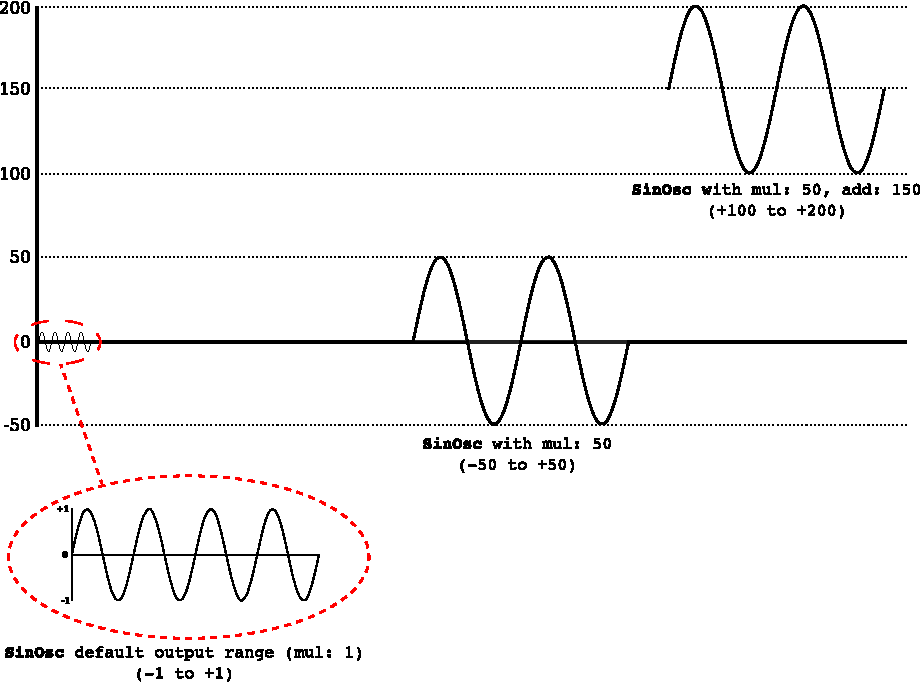
\includegraphics[scale=0.6]{fig-mul-add-scale.pdf}}}
\caption{Redimensionando âmbitos de UGens com mul e add}
\label{fig:mul-add-scale}
\end{figure}

\subsection{\texttt{linlin} e seus amigos}

Para qualquer outro redimensionamento arbitrário de âmbitos, você pode usar os práticos métodos \texttt{linlin}, \texttt{linexp}, \texttt{explin} e \texttt{expexp}. Os nomes nos métodos dão uma dica do que eles fazem: converter um âmbito linear em outro âmbito linear (\texttt{linlin}), linear para exponencial (\texttt{linexp}), etc.

\begin{lstlisting}[style=SuperCollider-IDE, basicstyle=\scttfamily\footnotesize]
// Um punhado de números
a = [1, 2, 3, 4, 5, 6, 7];
// Redimensione para 0-127, linear para linear
a.linlin(1, 7, 0, 127).round(1);
// Redimensione para 0-127, linear para exponencial
a.linexp(1, 7, 0.01, 127).round(1); // não use zero para um âmbito exponencial
\end{lstlisting}

Para uma revisão acerca de linear e exponencial, procure online a diferença entre progressões aritméticas e geométricas. Brevemente, sequências lineares (aritméticas) são como "1, 2, 3, 4, 5, 6" or "3, 6, 9, 12, 15", etc; e sequências exponenciais (geométricas) são como "1, 2, 4, 8, 16, 32" or "3, 9, 27, 81, 243", etc.




\section{Parando sintetizadores individualmente}

Eis um jeito bastante comum de iniciar diversos sintetizadores e ser capaz de interrompê-los separadamente. O exemplo é autoexplicativo:

\begin{lstlisting}[style=SuperCollider-IDE, basicstyle=\scttfamily\footnotesize]
// Rode uma linha de cada vez (não pare o som entre elas):
a = { Saw.ar(LFNoise2.kr(8).range(1000, 2000), mul: 0.2) }.play;
b = { Saw.ar(LFNoise2.kr(7).range(100, 1000), mul: 0.2) }.play;
c = { Saw.ar(LFNoise0.kr(15).range(2000, 3000), mul: 0.1) }.play;
// Pare os sintetizadores individualmente:
a.free;
b.free;
c.free; 	
\end{lstlisting}

\section{A mensagem \texttt{set}}

Assim como com qualquer função (reveja a seção \ref{sec:functions}), argumentos especificados no início da sua função de sintetizador ficam acessíveis ao usuário. Isso permite que você modifique parâmetros em tempo real (enquanto o sintetizador está rodando). A mensagem \texttt{set} ("definir") é usada para este fim. Exemplo simples:

\begin{lstlisting}[style=SuperCollider-IDE, basicstyle=\scttfamily\footnotesize]
x = {arg freq = 440, amp = 0.1; SinOsc.ar(freq, 0, amp)}.play;
x.set(\freq, 778);
x.set(\amp, 0.5);
x.set(\freq, 920, \amp, 0.2);
x.free;
\end{lstlisting}

É um bom hábito fornecer valores pré-definidos (como 440 e 0.1 acima), de outra forma o sintetizador não vai tocar até que você defina um valor apropriado para os parâmetros 'vazios'.

\section{Audio Buses}
\label{sec:audiobus}

Audio buses are used for routing audio signals. They are like the channels of a mixing board. SuperCollider has 128 audio buses by default. There are also control buses (for control signals), but for now let's focus on Audio Buses only.\footnote{We will take a quick look at control buses in section \ref{sec:control-buses}.}

\begin{figure}[h!]
\centerline{
	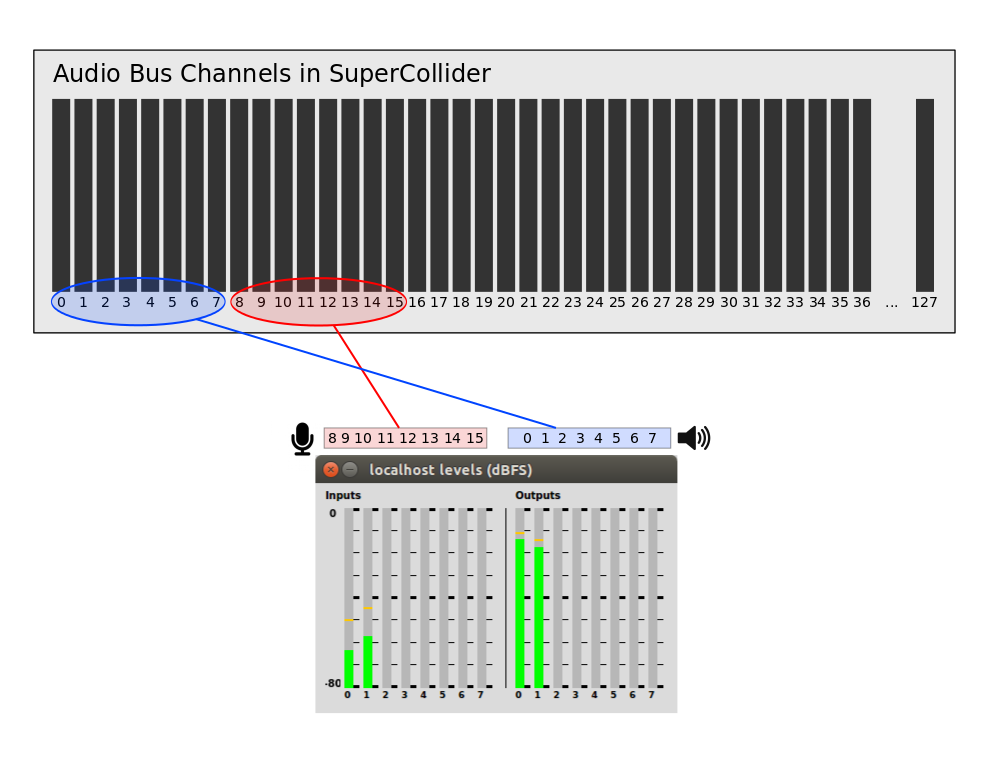
\includegraphics[scale=0.4]{fig-audio-bus.png}}
\caption{Audio buses and Meter window in SC.}
\label{fig:audio-bus}
\end{figure}

Hit [ctrl+M] to open up the Meter window. It shows the levels of all inputs and outputs. Figure \ref{fig:audio-bus} shows a screenshot of this window and its correspondence to SuperCollider's default buses. In SuperCollider, audio buses are numbered from 0 to 127. The first eight (0-7) are by default reserved to be the output channels of your sound card. The next eight (8-15) are reserved for the inputs of your sound card. All the others (16 to 127) are free to be used in any way you want, for example, when you need to route audio signals from one UGen to another.

\subsection{\texttt{Out} and \texttt{In} UGens}

Now try the following line of code:

\begin{lstlisting}[style=SuperCollider-IDE, basicstyle=\scttfamily\footnotesize]
{Out.ar(1, SinOsc.ar(440, 0, 0.1))}.play; // right channel
\end{lstlisting}

The \texttt{Out} UGen takes care of routing signals to specific buses.

The first argument to \texttt{Out} is the target bus, that is, where you want this signal to go.  In the example above, the number \texttt{1} means that we want to send the signal to bus 1, which is the right channel of your sound card.

The second argument of \texttt{Out.ar} is the actual signal that you want to ``write'' into that bus. It can be a single UGen, or a combination of UGens. In the example, it is just a sine wave. You should hear it only on your right speaker (or on your right ear if using headphones).

With the Meter window open and visible, go ahead and change the first argument of \texttt{Out.ar}: try any number between 0 and 7, and watch the meters. You will see that the signal goes wherever you tell it to.

\bigskip
\todo[inline, color=green!40]{ TIP: Most likely you have a sound card that can only play two channels (left and right), so you will only hear the sine tone when you send it to bus 0 or bus 1. When you send it to other buses (3 to 7), you will still see the corresponding meter showing the signal: SC is in fact sending the sound to that bus, but unless you have an 8-channel sound card you will not be able to hear the output of buses 3-7.}
\bigskip

One simple example of an audio bus being used for an effect is shown below.

\begin{lstlisting}[style=SuperCollider-IDE, basicstyle=\scttfamily\footnotesize]
// start the effect
f = {Out.ar(0, BPF.ar(in: In.ar(55), freq: MouseY.kr(1000, 5000), rq: 0.1))}.play;
// start the source
n = {Out.ar(55, WhiteNoise.ar(0.5))}.play;
\end{lstlisting}

The first line declares a synth (stored into the variable \texttt{f}) consisting of a filter UGen (a Band Pass Filter). A band pass filter takes any sound as input, and \emph{filters out all frequencies except the one frequency region that you want to let through}. \texttt{In.ar} is the UGen we use to read from an audio bus; so with \texttt{In.ar(55)} being used as input of the \texttt{BPF}, any sound that we send to bus 55 will be passed to the band pass filter. Notice that this first synth does not make any sound at first: when you evaluate the first line, bus 55 is still empty. It will only make sound when we send some audio into bus 55, which happens on the second line. 

The second line creates a synth and stores it into the variable \texttt{n}. This synth simply generates white noise, and outputs it \emph{not to the loudspeakers directly, but to audio bus 55 instead}. That is precisely the bus that our filter synth is listening to, so as soon as you evaluate the second line, you should start hearing the white noise being filtered by synth \texttt{f}.
In short, the routing looks like this:

\begin{center}
\emph{noise synth} $\rightarrow$ \emph{bus 55} $\rightarrow$ \emph{filter synth}
\end{center}

The order of execution is important. The previous example won't work if you evaluate the source \emph{before} the effect. This will be discussed in more detail in section \ref{sec:order-of-execution}, ``Order of Execution.''

One last thing: when you wrote in earlier examples synths like \texttt{\{SinOsc.ar(440)\}.play}, SC was actually doing \texttt{\{Out.ar(0, SinOsc.ar(440))\}.play} under the hood: it assumed you wanted to send the sound out to bus 0, so it automatically wrapped the first UGen with an \texttt{Out.ar(0, ...)} UGen. In fact a few more things are happening there behind the scenes, but we'll come back to this later (section \ref{sec:synthdef}).
\section{Entrada de Microfone}

O exemplo abaixo mostra como você pode facilmente acessar a entrada da sua placa de som com a UGen \texttt{SoundIn}.\footnote{Sabendo que \texttt{In.ar} lê o sinal de qualquer canal indicado, e sabendo que as entradas da sua placa de som são por padrão assinaladas para os canais 8-15 do SC, você poderia escrever \texttt{In.ar(8)} para obter som do seu microfone. Isso funciona perfeitamente bem, mas \texttt{SoundIn.ar} é uma opção mais conveniente.}

\begin{lstlisting}[style=SuperCollider-IDE, basicstyle=\scttfamily\footnotesize]
// Aviso: use fones de ouvido para evitar microfonia
{SoundIn.ar(0)}.play; // o mesmo que In.ar(8): recebe som do primeiro canal de entrada

// Versão estéreo
{SoundIn.ar([0, 1])}.play; // primeira e segunda entradas

// Um pouco de reverb só para animar?
{FreeVerb.ar(SoundIn.ar([0, 1]), mix: 0.5, room: 0.9)}.play;
\end{lstlisting}

\section{Expansão Multicanal}

Com sua janela Meter aberta---[ctrl+M]---, observe isso.

\begin{lstlisting}[style=SuperCollider-IDE, basicstyle=\scttfamily\footnotesize]
{Out.ar(0, Saw.ar(freq: [440, 570], mul: Line.kr(0, 1, 10)))}.play;
\end{lstlisting}

Estamos utilizando uma simpática UGen \texttt{Line.kr} para aumentar a amplitude de 0 a 1 em 10 segundos. Isso é bacana. Mas há outras mágicas interessantes acontecendo aqui. Você percebeu que há dois canais de saída (esquerdo e direito)? Você ouviu que há uma nota diferente em cada canal? Que que estas duas notas vêm de um \emph{list}---[440, 570]---que passa para o \texttt{Saw.ar} como argumento \texttt{freq}?

Isto se chama Expansão Multicanal.

David Cottle brinca que "expansão multicanal é uma [aplicação de arrays] que beira o vodu"\footnote{Cottle, D. ``Beginner's Tutorial.'' The SuperCollider Book, MIT Press, 2011, p. 14} Esta é uma das características do SuperCollider mais poderosas e únicas. E também uma que mais intriga as pessoas no início.

Em poucas palavras: se você utilizar um array como qualquer argumento de uma UGen, \emph{todo o patch é duplicado}. O número de cópias criado é \textit{o número de itens no array}. Estas UGens são enviadas para tantos \textit{canais adjacentes} quanto for necessário, começando pelo primeiro canal especificado como primeiro argumento de \texttt{Out.ar}.

No exemplo acima, temos \texttt{Out.ar(0, ... )}. O \texttt{freq} da onda dente-de-serra ("Saw") é um array de dois itens: \texttt{[440, 570]}. O que o SC faz? Ele "expande multicanal", criando duas cópias de todo o patch. A primeira cópia é uma onda dente-de-serra com uma frequência de 440 Hz, enviada para o canal 0 (seu canal esquerdo); a segunda cópia é uma dente-de-serra com uma frequência de 570 Hz, enviada para o canal 1 (seu canal direito)!

Vamos lá e verifique você mesmo. Mude estas duas frequências para qualquer outros valores que você quiser. Escute os resultados. Um vai para o canal esquerdo e o outro vai para o direito. Vá além e adicione uma terceira frequência para a lista (digamos, \texttt{[440, 570, 980]}). Observe a janela Meter. Você verá que as três primeiras saídas estão acendendo (mas você só conseguirá ouvir a terceira se tiver uma placa de som multicanal).

Além disso: você pode usar arrays adicionais em outros argumentos da mesma UGen ou em argumentos de outras UGens no mesmo sintetizador. O SuperCollider vai manter a casa em ordem e gerar sintetizadores que seguem estes valores corretamente. Por exemplo: agora ambas as frequências [440, 570] estão entrando suavemente ("fade in") de 0 a 1 em 10 segundos. Mas mude o código para \texttt{Line.kr(0, 1, [1, 15])} e você fará com que o som de 440 Hz demore 1 segundo para crescer e o de 570 Hz leve 15. Experimente.

Exercício: escute esta simulação de um "sinal de ocupado" de um telefone antigo. Ela usa a expansão multicanal para criar dois osciladores senoidais, cada um tocando uma frequência em um canal diferente. Faça o canal esquerdo pulsar 2 vezes por segundo e o canal direito pulsar 3 vezes por segundo. \endnote{Solução: \texttt{a = \{Out.ar(0, SinOsc.ar(freq: [800, 880], mul: LFPulse.ar([2, 3])))\}.play;}}

\medskip
\begin{lstlisting}[style=SuperCollider-IDE, basicstyle=\scttfamily\footnotesize]
a = {Out.ar(0, SinOsc.ar(freq: [800, 880], mul: LFPulse.ar(2)))}.play;
a.free;
\end{lstlisting}

\section{O objeto Bus}
\label{sec:busobject}

Aqui está um exemplo que utiliza tudo o que você aprendeu nas duas seções anteriores: canais de áudio e expansão multicanal.
 
\begin{lstlisting}[style=SuperCollider-IDE, basicstyle=\scttfamily\footnotesize]
// Rode isso primeiro (‘ligar reverb' -- inicialmente você não vai ouvir nada)
r = {Out.ar(0, FreeVerb.ar(In.ar(55, 2), mix: 0.5, room: 0.9, mul: 0.4))}.play;

// Agora rode isto em seguida (‘envie o sinal de ocupado para o canal de reverb')
a = {Out.ar(55, SinOsc.ar([800, 880], mul: LFPulse.ar(2)))}.play;
a.free;
\end{lstlisting}
 

Graças à expansão multicanal, o sinal de ocupado usa dois canais. Quando (no sintetizador \texttt{a}) enviamos o sinal de ocupado para o canal 55, na verdade, dois canais estão sendo utilizados---o número 55 e o canal imediatamente adjacente, 56. No reverb (sintetizador \texttt{r}), indicamos com \texttt{In.ar(55, 2)} que queremos ler 2 canais, começando pelo canal 55: então tanto 55 quanto 56 vão entrar no reverb. A saída do reverb também é expandida para dois canais, de maneira que o sintetizador \texttt{r} manda som para os canais 0 e 1 (canais esquerdo e direito da sua placa de som).

Bem, esta escolha de canal (55) para conectar uma fonte sonora a um efeito foi arbitrária: poderia ter sido qualquer outro número entre 16 e 127 (lembre-se, canis 0-15 são reservados para a as saídas e entradas da placa de som). Como seria inconveniente termos que ficar monitorando estes números. Logo que nossos patches ficarem mais complexos, imagine que pesadelo: “Qual foi mesmo o canal que escolhi para o reverb? Era 59 ou 95? E o canal do meu delay? Será que era 27? Não lembro...” e assim por diante.

O SuperCollider toma conta disso para você com objetos Bus. Apenas definimos manualmente o infame canal 55 nos exemplos acima como forma de demonstração. No nosso dia-a-dia com o SuperCollider, você deveria simplesmente usar o objeto Bus. O objeto Bus faz o trabalho de escolher um canal disponível para você e monitorá-lo. Eis como o utilizamos:

 
\begin{lstlisting}[style=SuperCollider-IDE, basicstyle=\scttfamily\footnotesize]
// Criar o bus
~meuBus = Bus.audio(s, 2);
// Ligar o reverb: ler de ~meuBus (fonte sonora)
r = {Out.ar(0, FreeVerb.ar(In.ar(~meuBus, 2), mix: 0.5, room: 0.9, mul: 0.4))}.play;
// Alimente o ~meuBus com o sinal de ocupado
b = {Out.ar(~meuBus, SinOsc.ar([800, 880], mul: LFPulse.ar(2)))}.play;
// Libere ambos os sintetizadores
r.free; b.free;
\end{lstlisting}
 

O primeiro argumento do \texttt{Bus.audio} é a variável \texttt{s}, que representa o servidor. O segundo argumento é quantos canais você precisa (2 no exemplo). Então você armazena isso em uma variável com um nome significativo (\texttt{$\sim$meuBus} no exemplo, mas poderia ser \texttt{$\sim$reverbBus}, \texttt{$\sim$fonte}, \texttt{$\sim$tangerina} ou o que fizer sentido para você dentro do seu patch). Depois disso, sempre que você precisar se referir àquele bus, apenas use a variável que você criou.

\section{Panning}

Panning is the spreading of an audio signal into a stereo or multichannel sound field. Here's a mono signal bouncing between left and right channel thanks to \texttt{Pan2}:\footnote{For multichannel panning, take a look at \texttt{Pan4} and \texttt{PanAz}. Advanced users may want to take a look at SuperCollider plug-ins for Ambisonics.}
\begin{lstlisting}[style=SuperCollider-IDE, basicstyle=\scttfamily\footnotesize]
p = {Pan2.ar(in: PinkNoise.ar, pos: SinOsc.kr(2), level: 0.1)}.play;
p.free;
\end{lstlisting}
From the \texttt{Pan2} Help file, you can see that the argument \texttt{pos} (position) expects a number between -1 (left) and +1 (right), 0 being center. That's why you can use a \texttt{SinOsc} directly into that argument: the sine oscillator is a bipolar UGen, so it outputs numbers between -1 and +1 by default.

Here's a more elaborated example. A sawtooth wave goes through a very sharp band pass filter (\texttt{rq: 0.01}). Notice the use of local variables to modularize different parts of the code. Analyze and try to understand as much as you can in the example above. Then answer the questions below.

\begin{lstlisting}[style=SuperCollider-IDE, basicstyle=\scttfamily\footnotesize]
(
x = {
	var lfn = LFNoise2.kr(1);
	var saw = Saw.ar(
		freq: 30, 
		mul: LFPulse.kr(
			freq: LFNoise1.kr(1).range(1, 10),
			width: 0.1));
	var bpf = BPF.ar(in: saw, freq: lfn.range(500, 2500), rq: 0.01, mul: 20);
	Pan2.ar(in: bpf, pos: lfn);
}.play;
)
x.free;
\end{lstlisting}
 
Questions:
\begin{enumerate}[(a)]
\item The variable \texttt{lfn} is used in two different places. Why? (What is the result?)
\item What happens if you change the \texttt{mul:} argument of the \texttt{BPF} from 20 to 10, 5, or 1? Why such a high number as 20 was used?
\item What part of the code is controlling the rhythm?
\end{enumerate}

Answers are at the end of this document.\endnote{(a) The variable \texttt{lfn} simply holds a \texttt{LFNoise2}. The role of \texttt{LFNoise2} in life is to generate a new random number every second (between -1 and +1), and slide to it from the previous random number (differently from \texttt{LFNoise0}, that jumps to the new number immediately). The first use of this variable \texttt{lfn} is in the \texttt{freq} argument of the BPF: \texttt{lfn.range(500, 2500)}. This takes the numbers between -1 and +1 and scales them to the range 500-2500. These numbers are then used as the center frequency of the filter. These frequencies are the pitches that we hear sliding up and down. Finally, \texttt{lfn} is used again to control the position of the panner \texttt{Pan2}. It is used directly (without a \texttt{.range} message) because the numbers are already in the range we want (-1 to +1). The nice result of this is that we couple the change of frequency with the change of position. How? Every second, \texttt{LFNoise2} starts to slide toward a new random number, and this becomes a synchronized change in frequency of the filter and panning position. If we had two different \texttt{LFNoise2} in each place, the changes would be uncorrelated (which might be fine too, but it's a different aural result). \\
(b) a \texttt{mul:} of 1 would just be too soft. Because the filter is so sharp, it takes so much out of the original signal that the amplitude drops too much. We need to boost the signal back to a reasonably audible range, so that's why we have \texttt{mul: 20} at the end of the \texttt{BPF} line. \\
(c) The rhythm is driven by the \texttt{LFPulse} that is the \texttt{mul:} argument of the \texttt{Saw}. \texttt{LFPulse} frequency (how many pulses per second) is controlled by an \texttt{LFNoise1} that produces numbers between 1 and 10 (interpolating between them). Those numbers are the ``how many notes per second'' of this patch.  
}
\section{Mix e Splay}

Este é um truque bacana. Você pode usar expansão multicanal para gerar sons complexos e depois mixá-los todos para mono ou estéreo com \texttt{Mix} ou \texttt{Splay}:
 
\begin{lstlisting}[style=SuperCollider-IDE, basicstyle=\scttfamily\footnotesize]
// saída com 5 canais (veja a janela Meter)
a = { SinOsc.ar([100, 300, 500, 700, 900], mul: 0.1) }.play;
a.free;
// Mixe em mono:
b = { Mix(SinOsc.ar([100, 300, 500, 700, 900], mul: 0.1)) }.play;
b.free;
// Mixe em estéreo (distribuição uniforme da esquerda para a direita)
c = { Splay.ar(SinOsc.ar([100, 300, 500, 700, 900], mul: 0.1)) }.play;
c.free
// Divirta-se com Splay:
(
d = {arg fundamental = 110;
	var harmonicos = [1, 2, 3, 4, 5, 6, 7, 8, 9];
	var som = BPF.ar(
		in: Saw.ar(32, LFPulse.ar(harmonicos, width: 0.1)),
		freq: harmonicos * fundamental,
		rq: 0.01,
		mul: 20);
	Splay.ar(som);	
}.play;
)
d.set(\fundamental, 100); // mude a fundamental apenas pela diversão
d.free;
\end{lstlisting}
 
Você consegue ver a expansão multicanal funcionando com este último exemplo de \texttt{Splay}? A única diferença é que o array é primeiro armazenado em uma variável (\texttt{harmonicos}) antes de se utilizada nas UGens. O array \texttt{harmonicos} tem 9 items, então o sintetizador irá se expandir para 9 canais. Então, um pouco antes de \texttt{.play}, \texttt{Splay} recebe o array de 9 canais e os mixa em estéreo, distribuindo os canais uniformemente da esquerda para a direita.\footnote{A última linha antes do \texttt{.play} poderia ser explicitamente escrita como \texttt{Out.ar(0, Splay.ar(som))}. Lembre-se que o SuperCollider está gentilmente preenchendo as lacunas e inserindo aí um
\texttt{Out.ar(0...)}---é assim que o sintetizador sabe que deve tocar nos canais esquerdo (bus 0) e direito (bus a).}

\texttt{Mix} tem um outro truque interessante: o método \texttt{fill}. De uma só vez, ele cria um array de sintetizadores e os mixa em mono.

\begin{lstlisting}[style=SuperCollider-IDE, basicstyle=\scttfamily\footnotesize]
// Gerador instantâneo de clusters
c = { Mix.fill(16, {SinOsc.ar(rrand(100, 3000), mul: 0.01)}) }.play;
c.free;
// Uma nota com 12 parciais com amplitudes decrescentes
(
n = { Mix.fill(12, {arg contador;
	var parcial = contador + 1; // queremos começar do 1, não do 0
	SinOsc.ar(parcial * 440, mul: 1/parcial.squared) * 0.1
	})
}.play;
FreqScope.new;
)
n.free;
\end{lstlisting}

Você fornece duas coisas para o \texttt{Mix.fill}: o tamanho do array e uma função (entre chaves) que será utilizada para preencher o array. No primeiro exemplo acima, \texttt{Mix.fill} executa a função 16 vezes. Note que a função inclui um componente variável: a frequência do oscilador senoidal que pode ser qualquer número entre 100 e 3000. Dezesseis senoides serão criadas, cada uma com uma frequência aleatória diferente. Todas elas serão mixadas em mono e você ouvirá o resultado no seu canal esquerdo.
O segundo exemplo mostra que a função pode receber um argumento de "contador" que monitora o número de iterações (como em \texttt{Array.fill}). 
Doze osciladores senoidais são gerados seguindo a série harmônica e mixados como uma única nota em mono.

\section{Playing an audio file}

First, you have to load the sound file into a buffer. The second argument to \texttt{Buffer.read} is the path of your sound file between double quotes. You will need to change that accordingly so that it points to a WAV or AIFF file on your computer. After buffers are loaded, simply use the \texttt{PlayBuf} UGen to play them back in various ways.

\bigskip
\todo[inline, color=green!40]{ TIP: A quick way to get the correct path of a sound file saved on your computer is drag the file onto a blank SuperCollider document. SC will give you the full path automatically, already in double quotes! }
\bigskip

\begin{lstlisting}[style=SuperCollider-IDE, basicstyle=\scttfamily\footnotesize]
// Load files into buffers:
~buf1 = Buffer.read(s, "/home/Music/wheels-mono.wav"); // one sound file
~buf2 = Buffer.read(s, "/home/Music/mussorgsky.wav"); // another sound file

// Playback:
{PlayBuf.ar(1, ~buf1)}.play; // number of channels and buffer
{PlayBuf.ar(1, ~buf2)}.play;

// Get some info about the files:
[~buf1.bufnum, ~buf1.numChannels, ~buf1.path, ~buf1.numFrames];
[~buf2.bufnum, ~buf2.numChannels, ~buf2.path, ~buf2.numFrames];

// Changing playback speed with 'rate'
{PlayBuf.ar(numChannels: 1, bufnum: ~buf1, rate: 2, loop: 1)}.play;
{PlayBuf.ar(1, ~buf1, 0.5, loop: 1)}.play; // play at half the speed
{PlayBuf.ar(1, ~buf1, Line.kr(0.5, 2, 10), loop: 1)}.play; // speeding up
{PlayBuf.ar(1, ~buf1, MouseY.kr(0.5, 3), loop: 1)}.play; // mouse control

// Changing direction (reverse)
{PlayBuf.ar(1, ~buf2, -1, loop: 1)}.play; // reverse sound
{PlayBuf.ar(1, ~buf2, -0.5, loop: 1)}.play; // play at half the speed AND reversed
\end{lstlisting}

\section{Nós ("nodes") de sintetizador}

Nos exemplos anteriores com \texttt{PlayBuf}, você teve que apertar [ctrl+.] depois de cada linha para parar o som. Em outros exemplos, você atribuiu o sintetizador a uma variável (como \texttt{x = \{WhiteNoise.ar\}.play}) para que você pudesse pará-lo diretamente com \texttt{x.free}.

Toda vez que você cria um sintetizador no SuperCollider, você sabe que ele roda no servidor, nosso "motor sonoro". Cada sintetizador que está rodando no servidor é representado por um \emph{node} ("nó" ou "nódulo"). Podemos dar uma espiada nesta árvore de nós com o comando \texttt{s.plotTree}. Experimente. Uma janela chamada \texttt{NodeTree} ("Árvore de nós") vai abrir.

 
\begin{lstlisting}[style=SuperCollider-IDE, basicstyle=\scttfamily\footnotesize]
// abra a GUI
s.plotTree;
// rode estes um por um (não pare o som) e observe a Node Tree:
w = { SinOsc.ar(60.midicps, 0, 0.1) }.play;
x = { SinOsc.ar(64.midicps, 0, 0.1) }.play;
y = { SinOsc.ar(67.midicps, 0, 0.1) }.play;
z = { SinOsc.ar(71.midicps, 0, 0.1) }.play;
w.free;
x.free;
y.free;
z.free;
\end{lstlisting}
 

Cada retângulo que você vê na Node Tree é um nó de sintetizador. Cada sintetizador ganha um nome temporário (algo como temp\_101, temp\_102, etc.) e fica ali enquanto estiver rodando. Experimente agora tocar novamente as quatro senoides e aperte [ctrl+.] (observe a janela Node Tree). O atalho [ctrl+.] impiedosamente interrompe todos os nós que estão rodando no servidor. Por outro lado, com o método \texttt{.free}, você pode ser mais sutil e liberar nós específicos, um de cada vez.

Uma coisa importante de se perceber é que sintetizadores podem continuar a rodar no servidor mesmo que eles estejam gerando apenas silêncio. Eis um exemplo. A amplitude desta UGen \texttt{WhiteNoise} irá de 0.2 a 0 em dois segundos. Depois disso, não escutaremos nada. Mas você vê que o nó do sintetizador ainda esta ali e não desaparecerá até que você o libere.

 
\begin{lstlisting}[style=SuperCollider-IDE, basicstyle=\scttfamily\footnotesize]
// Execute e observe a janela Node Tree window por alguns segundos
x = {WhiteNoise.ar(Line.kr(0.2, 0, 2))}.play;
x.free;
\end{lstlisting}
 

\subsection{O glorioso doneAction: 2}

Felizmente, há uma maneira de criar sintetizadores mais espertos neste sentido: por exemplo, não seria ótimo se pudéssemos pedir ao \texttt{Line.kr} para notificar o sintetizador quando ele tiver terminado seu trabalho (a rampa de 0.2 a 0), e então o sintetizador se liberasse automaticamente?

Insira o argumento \texttt{doneAction: 2} para resolver todos os nossos problemas.

Toque os exemplos abaixo e compare como eles se comportam com e sem doneAction: 2. Continue observando a Node Tree enquanto você roda as linhas.
 
\begin{lstlisting}[style=SuperCollider-IDE, basicstyle=\scttfamily\footnotesize]
// sem doneAction: 2
{WhiteNoise.ar(Line.kr(0.2, 0, 2))}.play;
{PlayBuf.ar(1, ~buf1)}.play; // PS. isso presume que você anda tem seu arquivo de som carregado no ~buf1 da seção anterior

// com doneAction: 2
{WhiteNoise.ar(Line.kr(0.2, 0, 2, doneAction: 2))}.play;
{PlayBuf.ar(1, ~buf1, doneAction: 2)}.play;
\end{lstlisting}
 
Os sintetizadores com doneAction: 2 vão se liberar automaticamente logo que seu trabalho estiver feito (isto é, assim que a rampa do \texttt{Line.kr} tiver terminado no primeiro exemplo e logo que o \texttt{PlayBuf.ar} tiver terminado de tocar o arquivo de som no segundo exemplo). Confirme que você entendeu este conceito, pois ele será bastante útil na próxima seção: Envelopes.

\section{Envelopes}

Até agora, a maioria dos nossos exemplos foi de sons contínuos. Já está na hora de aprender a modelar o envelope de amplitude de um som. Um bom exemplo para começar é um envelope percussivo. Imagine um ataque em um prato suspenso. O tempo que o som leva para ir do silêncio à amplitude máxima é muito curto---alguns milissegundos talvez. Isto é chamado \emph{tempo de ataque}. O tempo que leva para o som do prato diminuir da máxima amplitude de volta ao silêncio (zero) é um pouco mais longo, talvez alguns segundos. Isto é chamado o \emph{tempo de repouso}.

Pense em um envelope de amplitude simplesmente como um número que muda ao longo do tempo e pode ser utilizado como o multiplicador (\texttt{mul}) de qualquer UGen que produz som. Estes números devem estar entre 0 (silêncio) e 1 (amplitude máxima), porque é assim que o SuperCollider entende a amplitude. Talvez agora você se dê conta de que o último exemplo já continha um envelope de amplitude: em \texttt{\{WhiteNoise.ar(Line.kr(0.2, 0, 2, doneAction: 2))\}.play}, fazemos a amplitude do ruído branco ir de 0.2 a 0 em 2 segundos. Um \texttt{Line.kr}, no entanto, não é um tipo de envelope muito flexível.

\texttt{Env} é o objeto que você usará o tempo todo para definir todo tipo de envelopes. O \texttt{Env} tem muitos métodos úteis; só conseguiremos ver alguns deles aqui. Sinta-se à vontade para explorar a Ajuda de \texttt{Env} para aprender mais. 

\subsection{Env.perc}

\texttt{Env.perc} é uma maneira prática de conseguir um envelope percussivo. Ele aceita quatro argumentos:  attackTime, releaseTime, level e curve (que podemos traduzir como: "tempo de ataque, tempo de repouso, nível e curva"). Vejamos algumas formas típicas, ainda fora de qualquer sintetizador.

\begin{lstlisting}[style=SuperCollider-IDE, basicstyle=\scttfamily\footnotesize]
Env.perc.plot; // usando todos os argumentos padrão
Env.perc(0.5).plot; // attackTime: 0.5
Env.perc(attackTime: 0.3, releaseTime: 2, level: 0.4).plot;
Env.perc(0.3, 2, 0.4, 0).plot; // o mesmo que acima, mas curve:0 produz uma linha reta
\end{lstlisting}
 
Agora simplesmente o encaixamos dentro de um sintetizador:

\begin{lstlisting}[style=SuperCollider-IDE, basicstyle=\scttfamily\footnotesize]
{PinkNoise.ar(Env.perc.kr(doneAction: 2))}.play; // argumentos padrão do Env.perc
{PinkNoise.ar(Env.perc(0.5).kr(doneAction: 2))}.play; 
{PinkNoise.ar(Env.perc(0.3, 2, 0.4).kr(2))}.play;
{PinkNoise.ar(Env.perc(0.3, 2, 0.4, 0).kr(2))}.play;
\end{lstlisting}
 
Tudo o que você tem de fazer é adicionar \texttt{.kr(doneAction: 2)} logo depois de \texttt{Env.perc} e pronto. Na verdade, neste caso você pode até remover a declaração explícita do argumento doneAction e simplesmente ficar com \texttt{.kr(2)}. O \texttt{.kr} está esta dizendo para o SC rodar este envelope na velocidade da taxa de controle (como outros sinais de controle que vimos antes).

\subsection{Env.triangle}

\texttt{Env.triangle} recebe apenas dois argumentos: duração e nível. Exemplos:

 
\begin{lstlisting}[style=SuperCollider-IDE, basicstyle=\scttfamily\footnotesize]
// Veja-o:
Env.triangle.plot;
// Ouça-o:
{SinOsc.ar([440, 442], mul: Env.triangle.kr(2))}.play;
// Aliás, um envelope pode ser um multiplicador em qualquer lugar do seu código:
{SinOsc.ar([440, 442]) * Env.triangle.kr(2)}.play;
\end{lstlisting}

\subsection{Env.linen}

\texttt{Env.linen} descreve um envelope linear com ataque, porção de sustentação e repouso. Você também pode especificar o nível e tipo de curva. Exemplo:

\begin{lstlisting}[style=SuperCollider-IDE, basicstyle=\scttfamily\footnotesize]
// Veja-o:
Env.linen.plot;
// Ouça-o:
{SinOsc.ar([300, 350], mul: Env.linen(0.01, 2, 1, 0.2).kr(2))}.play;
\end{lstlisting}

\subsection{Env.pairs}

Precisa de mais flexibilidade? Com \texttt{Env.pairs} você pode ter envelopes com qualquer forma e duração que quiser. \texttt{Env.pairs} recebe dois argumentos: um arranjo ("array") de pares de [tempo, nível] e um tipo de curva (veja na Ajuda de Env todos os tipos de curva disponíveis).

 
\begin{lstlisting}[style=SuperCollider-IDE, basicstyle=\scttfamily\footnotesize]
(
{
	var env = Env.pairs([[0, 0], [0.4, 1], [1, 0.2], [1.1, 0.5], [2, 0]], \lin);
	env.plot;
	SinOsc.ar([440, 442], mul: env.kr(2));
}.play;
)
\end{lstlisting}
 
Leia o arranjo de pares assim:
\begin{center}
No tempo 0, esteja no nível 0;\\
No tempo 0.4, esteja no nível 1;\\
No tempo 1, esteja no nível 0.2;\\
No tempo 1.1, esteja no nível 0.5;\\
No tempo 2, esteja no nível 0;
\end{center}

\subsubsection{Envelopes---não apenas para amplitude}

Nada impede você de usar as estas mesmas formas para controlar algo além da amplitude. Você só precisa escaloná-las para o âmbito de números desejado. Por exemplo, Você pode criar um envelope para controlar a mudança de frequências ao longo do tempo:

\begin{lstlisting}[style=SuperCollider-IDE, basicstyle=\scttfamily\footnotesize]
(
{
	var freqEnv = Env.pairs([[0, 100], [0.4, 1000], [0.9, 400], [1.1, 555], [2, 440]], \lin);
	SinOsc.ar(freqEnv.kr, mul: 0.2);
}.play;
)
\end{lstlisting}

Envelopes são uma maneira poderosa de controlar qualquer parâmetro de um sintetizador que precisa variar ao longo do tempo.

\subsection{Envelope ADSR}

Todos os envelopes vistos até agora têm uma coisa em comum: eles têm uma duração fixa, pré-definida. Há situações, no entanto, em que este tipo de envelope não é adequado. Por exemplo, imagine que você está tocando em um teclado MIDI. o \textit{ataque} da nota é disparado quando você pressiona a tecla. O \textit{repouso}, quando você tira seu dedo da tecla. Mas a quantidade de tempo que você permanece com o dedo sobre a tecla não é conhecido de antemão. O que precisamos neste caso é de um "envelope sustentado". Em outras palavras, depois da porção de ataque, o envelope precisa segurar a nota por uma quantidade de tempo indefinida e apenas disparar a porção de repouso depois de algum sinal, ou mensagem--- isto é, o momento em que você "solta a tecla".

Um envelope ASR (Ataque, Sustentação, Repouso) se encaixa perfeitamente. Uma variação mais popular é o envelope ADSR (Ataque, Decaimento, Sustentação, Repouso). Vamos dar uma olhada nos dois.

 
\begin{lstlisting}[style=SuperCollider-IDE, basicstyle=\scttfamily\footnotesize]
// ASR
// Toque nota ('aperte tecla')
// attackTime: 0.5 seconds, sustainLevel: 0.8, releaseTime: 3 seconds
x = {arg gate = 1, freq = 440; SinOsc.ar(freq: freq, mul: Env.asr(0.5, 0.8, 3).kr(doneAction: 2, gate: gate))}.play;
// Pare nota ('tirar dedo da tecla' - ativar a porção de repouso)
x.set(\gate, 0); // uma alternativa é x.release

// ADSR (ataque, decaimento, sutentação, repouso)
// Toque nota:
(
d = {arg gate = 1;
	var snd, env;
	env = Env.adsr(0.01, 0.4, 0.7, 2);
	snd = Splay.ar(BPF.ar(Saw.ar((32.1, 32.2..33)), LFNoise2.kr(12).range(100, 1000), 0.05, 10));
	Out.ar(0, snd * env.kr(doneAction: 2, gate: gate));
}.play;
)
// Pare nota:
d.release; // isto é equivalente a d.set(\gate, 0);
\end{lstlisting}
 
Conceitos-chave:

\begin{description}
\item[Ataque ("Attack")] O tempo (em segundos) que leva para ir do silêncio (zero) até o pico de amplitude
\item[Decaimento ("Decay")] O tempo (em segundos) que leva para ir do pico de amplitude para a amplitude de sustentação
\item[Sustentação ("Sustain")] A amplitude (entre 0 e 1) na qual a nota é sustentada (importante: isto não tem nada a ver com tempo)
\item[Repouso ("Release")] O tempo (em segundos) que leva para ir do nível de sustentação para o zero (silêncio).
\end{description}

Como envelopes sustentados não tem uma duração total conhecida de antemão, eles precisam de uma notificação tanto de quando começar (disparar o ataque) e quando parar (disparar o repouso). Esta notificação é chamada um \emph{gate} ("portão"). O gate é o que diz para que o envelope se ‘abra’ (1) ou se ‘feche’ (0), portanto começando e terminando a nota.

Para que um envelope ASR ou ADSR funcione no seu sintetizador, você precisa declarar um argumento \texttt{gate}. Normalmente, o padrão é \texttt{gate = 1} porque você quer que o sintetizador comece logo a tocar. Quando você quer que o sintetizador pare, simplesmente mande uma mensagem \texttt{.release} ou \texttt{.set(\textbackslash gate, 0)}: a porção de repouso do envelope será então disparada. Por exemplo, se seu tempo de repouso é 3, a nota vai levar três segundos para se extinguir completamente \emph{desde o momento em que você enviou a mensagem} \texttt{.set(\textbackslash gate, 0)}. 

\subsection{EnvGen}

Vale registrar que a construção que você aprendeu nesta seção para gerar envelopes é um atalho, como mostrado no código abaixo.

\begin{lstlisting}[style=SuperCollider-IDE, basicstyle=\scttfamily\footnotesize]
// Isso:
{ SinOsc.ar * Env.perc.kr(doneAction: 2) }.play;
// ... é um atalho disso:
{ SinOsc.ar * EnvGen.kr(Env.perc, doneAction: 2) }.play;
\end{lstlisting}

\texttt{EnvGen} é a UGen que de fato toca os envelopes segmentados ("breakpoint envelopes") definidos por \texttt{Env}. Para todos os propósitos práticos, você pode continuar a usar o atalho. Mas é útil saber que estas notações são equivalentes, já que você muitas vezes verá  \texttt{EnvGen} sendo utilizado nos arquivos de Ajuda e outros exemplos online.

\section{Definições de sintetizador}
\label{sec:synthdef}

Até aqui, sem dificuldade alguma, pudemos \emph{definir} sintetizadores e fazê-los \emph{tocar} imediatamente. Para além disso, a mensagem \texttt{.set} nos deu alguma flexibilidade para alterar os controles do sintetizador em tempo real. No entanto, há situações em que você pode querer definir seus sintetizadores antes (sem tocá-los imediatamente) e tocá-los somente depois. Em essência, isso significa que temos de separar o momento de escrever a receita (a definição de sintetizador) do momento de assar o bolo (criar o som).


\subsection{SynthDef e Synth}

\texttt{SynthDef} é o que usamos para “escrever a receita” de um sintetizador. Depois você pode tocá-lo com \texttt{Synth}. Aqui está um exemplo simples.

\begin{lstlisting}[style=SuperCollider-IDE, basicstyle=\scttfamily\footnotesize]
// Definição de sintetizador com o objeto SynthDef
SynthDef("minhaSenoide1", {Out.ar(0, SinOsc.ar(770, 0, 0.1))}).add;
// Toque uma nota com o objeto Synth
x = Synth("minhaSenoide1");
x.free;

// Um exemplo ligeiramente mais flexível usando argumentos
// e um envelope com desligamento automático (doneAction: 2)
SynthDef("minhaSenoide2”, {arg freq = 440, amp = 0.1; 
	var env = Env.perc(level: amp).kr(2);
	var snd = SinOsc.ar(freq, 0, env);
	Out.ar(0, snd);
}).add;

Synth("minhaSenoide2"); // usando os valores pré-definidos;
Synth("minhaSenoide2", [\freq, 770, \amp, 0.2]);
Synth("minhaSenoide2", [\freq, 415, \amp, 0.1]);
Synth("minhaSenoide2", [\freq, 346, \amp, 0.3]);
Synth("minhaSenoide2", [\freq, rrand(440, 880)]);
\end{lstlisting}

O primeiro argumento para o \texttt{SynthDef} é um nome para o sintetizador definido pelo usuário. O segundo argumento é uma função na qual você especifica um gráfico de UGens (assim é chamada uma combinação de UGens). Note que você tem de usar \texttt{Out.ar} explicitamente para indicar para qual canal você quer enviar o sinal. Finalmente, o \texttt{SynthDef} recebe a mensagem  \texttt{.add} ao final, que diz que você está a adicionando a uma coleção de sintetizadores que o SC conhece. Isso é somente válido até você fechar o SuperCollider.

Depois que você criar uma ou mais definições de sintetizador com \texttt{SynthDef}, você pode tocá-las com \texttt{Synth}: o primeiro argumento é o nome do sintetizador que você quer usar e o segundo argumento (opcional) é um array com quaisquer parâmetros que você queira especificar (freq, amp, etc.)

\subsection{Exemplo}

Eis um exemplo mais longo. Depois que o SynthDef é adicionado, nós utilizamos um truque com um array para criar um acode de 6 notas com alturas e amplitudes aleatórias. Cada sintetizador é armazenado em uma das posições do array, para que possamos desligá-los individualmente. 
 
\begin{lstlisting}[style=SuperCollider-IDE, basicstyle=\scttfamily\footnotesize]
// Criar SynthDef
(
SynthDef(“uau”, {arg freq = 60, amp = 0.1, gate = 1, uaurelease = 3;
	var chorus, fonte, filtromod, env, som;
	chorus = Lag.kr(freq, 2) * LFNoise2.kr([0.4, 0.5, 0.7, 1, 2, 5, 10]).range(1, 1.02);
	fonte = LFSaw.ar(chorus) * 0.5;
	filtromod = SinOsc.kr(1/16).range(1, 10);
	env = Env.asr(1, amp, uaurelease).kr(2, gate);
	som = LPF.ar(in: fonte, freq: freq * filtromod, mul: env);
Out.ar(0, Splay.ar(som))
}).add;
)

// Observe a Node Tree
s.plotTree;

// Criar um acorde de 6 notas
a = Array.fill(6, {Synth(“uau”, [\freq, rrand(40, 70).midicps, \amp, rrand(0.1, 0.5)])}); // tudo em uma única linha

// Encerrar notas uma por uma
a[0].set(\gate, 0);
a[1].set(\gate, 0);
a[2].set(\gate, 0);
a[3].set(\gate, 0);
a[4].set(\gate, 0);
a[5].set(\gate, 0);

// AVANÇADO: rode o acorde de 6 notas novamente e depois execute esta linha.
// Você consegue imaginar o que está acontecendo?
SystemClock.sched(0, {a[5.rand].set(\freq, rrand(40, 70).midicps); rrand(3, 10)});
\end{lstlisting}

Para ajudá-lo a entender o SynthDef acima:

\begin{itemize}
\item O som resultante é a soma de sete osciladores dentes-de-serra com afinações muito próximas passando por um filtro passa-baixa (“low pass”).
\item Estes sete osciladores são criador por expansão multicanal.
\item O que é a variável \texttt{chorus}? É a frequência \texttt{freq} multiplicada por um \texttt{LFNoise2.kr}. Aqui começa a expansão multicanal, porque um array de 7 itens é fornecido como argumento para o LFNoise2. O resultado é que sete cópias do LFNoise2 são criadas, cada uma rodando a uma velocidade diferente retirada da lista \texttt{[0.4, 0.5, 0.7, 1, 2, 5, 10]}. Suas saídas são restritas ao âmbito de 1.0 a 1.02.
\item Como um atributo extra, note que \texttt{freq} está empacotado em um \texttt{Lag.kr}. Sempre que uma nova frequência alimenta o Synth, a UGen Lag simplesmente cria uma rampa entre o valor velho e o valor novo. O "lag time" (duração da rampa), neste caso, é 2 segundos. Isso é o que causa o efeito de glissando que você ouve após rodar a última linha do exemplo.  
\item A fonte sonora \texttt{LFSaw.ar} recebe a variável \texttt{chorus} como sua frequência. Em um exemplo concreto: para um valor \texttt{freq} de 60 Hz, a variável \texttt{chorus} resultaria em uma expressão como

$$60 * [1.01, 1.009, 1.0, 1.02, 1.015, 1.004, 1.019]$$

na qual os números da lista estariam constantemente subindo e descendo de acordo com as velocidades de cada LFNoise2. O resultado final é uma lista de sete frequências sempre deslizando entre 60 e 61.2 (60 * 1.02). Isso é chamado \textit{efeito chorus}, por isso o nome da variável. 
\item Quando a variável \texttt{chorus} é usada como freq de \texttt{LFSaw.ar}, acontece expansão multicanal: tempos agora sete ondas dentes-de-serra com frequências ligeiramente diferentes.
\item A variável \texttt{filtromod} é só um oscilador senoidal movendo-se muito lentamente (1 ciclo a cada 16 segundos), com seu âmbito de saída escalonado para 1-10. Isso será usado para modular a frequência de corte do filtro passa-baixa.
\item A variável \texttt{som} guarda o filtro passa-baixa (LPF), que recebe \texttt{fonte} como entrada e atenua todas as frequências acima de sua frequência de corte. Este corte não é um valor fixo: ele é a expressão \texttt{freq * filtromod}. Então no exemplo, ao assumir freq = 60, isso torna-se um número entre 60 e 600. Lembre-se que filtromod é um número oscilando entre 1 e 10, de maneira que a multiplicação seria 60 * (1 a 10).
\item \texttt{LPF} também expande multicanal para sete cópias. O envelope de amplitude \texttt{env} também é aplicado neste ponto.
\item Finalmente, \texttt{Splay} pega esse array de sete canais e mixa em estéreo.

\end{itemize}
 
\subsection{Nos bastidores}

Este processo em duas etapas de primeiro criar o SynthDef (com um nome próprio) e depois chamar um Synth é o que o SC faz o tempo quando você escreve comandos simples como \texttt{\{SinOsc.ar\}.play}. SuperCollider desdobra isso em (a) criar um SynthDef temporário e (b) tocá-lo imediatamente (essa é a razão dos nomes temp\_01, temp\_02 que você vê na Post window). Tudo isso nos bastidores, para sua conveniência.
 
\begin{lstlisting}[style=SuperCollider-IDE, basicstyle=\scttfamily\footnotesize]
// Quando você faz isso:
{SinOsc.ar(440)}.play;
//O que o SC está fazendo é isso:
{Out.ar(0, SinOsc.ar(440))}.play;
// O que por sua vez na verdade é isso:
SynthDef(“nomeTemporario", {Out.ar(0, SinOsc.ar(440))}).play;

// E todos eles são atalhos desta operação em duas etapas:
SynthDef(“nomeTemporario", {Out.ar(0, SinOsc.ar(440))}).add; // criar a definição de um sintetizador
Synth("nomeTemporario"); // tocá-lo
\end{lstlisting}

\section{Pbind pode tocar sua SynthDef}

Uma das belezas de se criar seus sintetizadores como \texttt{SynthDef}s é que você pode usar \texttt{Pbind} para tocá-los.

Assumindo que a SynthDef \texttt{"uau"} ainda esteja armazenado na memória (deveria estar, a não ser que você tenha fechado e reaberto o SC depois do último exemplo), experimente os \texttt{Pbind}s abaixo:

\begin{lstlisting}[style=SuperCollider-IDE, basicstyle=\scttfamily\footnotesize]
(
Pbind(
	\instrument, "uau",
	\degree, Pwhite(-7, 7),
	\dur, Prand([0.125, 0.25], inf),
	\amp, Pwhite(0.5, 1),
	\uaurelease, 1
).play;
)

(
Pbind(
	\instrument, "uau",
	\scale, Pstutter(8, Pseq([
		Scale.lydian,
		Scale.major,
		Scale.mixolydian,
		Scale.minor,
		Scale.phrygian], inf)),
	\degree, Pseq([0, 1, 2, 3, 4, 5, 6, 7], inf),
	\dur, 0.2,
	\amp, Pwhite(0.5, 1),
	\uaurelease, 4,
	\legato, 0.1
).play;
)
\end{lstlisting}
 
Ao usar \texttt{Pbind} para tocar um das suas \texttt{SynthDef}s personalizados, esteja atento aos seguintes pontos:

\begin{itemize}
\item Use a chave ("key") \texttt{\textbackslash instrument} do \texttt{Pbind} para declarar o nome da sua \texttt{SynthDef}.
\item Todos os argumentos da sua SynthDef são controláveis a partir do \texttt{Pbind}: simplesmente use-os como chaves do \texttt{Pbind}. Por exemplo, repare no argumento chamado \texttt{\textbackslash uaurelease} utilizado acima. Esta não é uma das chaves padrão entendidas pelo \texttt{Pbind}---ela só existe na definição do sintetizador  \texttt{uau} (o nome bobo foi escolhido de propósito).

\item Para utilizar todas as facildades de conversão de alturas do \texttt{Pbind} (as chaves \texttt{\textbackslash degree}, \texttt{\textbackslash note} e \texttt{\textbackslash midinote}), tenha certeza de que sua \texttt{SynthDef} tem um argumento de entrada \texttt{freq} (tem que ser escrito exatamente assim). Pbind fará os cálculos para você.
\item Se for usar um envelope sustentado como \texttt{Env.adsr}, garanta que seu sintetizador tenha o argumento padrão \texttt{gate = 1} (\texttt{gate} tem que ser excrito exatamente assim, porque o \texttt{Pbind} o utiliza nos bastidores para parar as notas nos momentos certos).
\item Se você não estiver usando um envelope sustentado, tenha certeza que sua SynthDef inclui um doneAction: 2 em uma UGen apropriada, para liberar automaticamente os nós de sintetizador no servidor.
\end{itemize}

Exercício: escreva um ou mais \texttt{Pbind}s para tocar a SynthDef \texttt{"pluck"} fornecida abaixo. Para o argumento \texttt{cordaAbafada}, tente valores entre  0.1 e 0.9. Faça com que seu \texttt{Pbind} toque uma sequência lenta de acordes. Tente arpejar os acordes com \texttt{\textbackslash strum}.

\begin{lstlisting}[style=SuperCollider-IDE, basicstyle=\scttfamily\footnotesize]
(
SynthDef("pluck", {arg amp = 0.1, freq = 440, decaimento = 5, cordaAbafada = 0.1;
var env, som;
env = Env.linen(0, decaimento, 0).kr(doneAction: 2);
som = Pluck.ar(
        in: WhiteNoise.ar(amp),
        trig: Impulse.kr(0),
        maxdelaytime: 0.1,
        delaytime: freq.reciprocal,
        decaytime: decaimento,
        coef: cordaAbafada);
    Out.ar(0, [som, som]);
}).add;
)
\end{lstlisting}

\section{Canais de Controle}
\label{sec:control-buses}

Em uma seção anterior deste tutorial, falamos sobre canais de áudio ("Audio Buses") (seção \ref{sec:audiobus}) e o objeto Bus (seção \ref{sec:busobject}). Naquele momento, escolhemos deixar de lado o tópico dos Canais de Controle ("Control Buses") para nos focarmos no conceito de roteamento de áudio.

Canais de controle no SuperCollider são para o roteamento de sinais de controle, não de áudio. Exceto por esta diferença, não há nenhuma outra distinção prática ou conceitual entre canais de áudio de de controle. Você cria e gerencia um canal de controle da mesma maneira que você faz com os canais de áudio, simplesmente usando \texttt{.kr} em vez de \texttt{.ar}. O SuperCollider tem  4096 canais de controle como padrão.

A primeira parte do exemplo abaixo usa um número de canal arbitrário apenas com a finalidade de demonstração. A segunda parte usa o objeto Bus, que é a maneira recomendada de criar canais.


\begin{lstlisting}[style=SuperCollider-IDE, basicstyle=\scttfamily\footnotesize]
// Escreva um sinal de controle no canal de controle 55
{Out.kr(55, LFNoise0.kr(1))}.play;
// Leia um sinal de controle do canal 55
{In.kr(55).poll}.play;

// Usando o objeto Bus
~meuCanalDeControle = Bus.control(s, 1);
{Out.kr(~meuCanalDeControle, LFNoise0.kr(5).range(440, 880))}.play;
{SinOsc.ar(freq: In.kr(~meuCanalDeControle))}.play;
\end{lstlisting}

O próximo exemplo mostra um único sinal de controle sendo utilizado para modular dois sintetizadores diferentes ao mesmo tempo. No sintetizador \texttt{Blip}, o sinal de controle é redimensionado para controlar o número de harmônicos entre 1 e 10. No segundo sintetizador, o mesmo sinal de controle é redimensionado para modular a frequência do oscilador \texttt{Pulse}.

\begin{lstlisting}[style=SuperCollider-IDE, basicstyle=\scttfamily\footnotesize]
// Crie o canal de controle
~meuControle = Bus.control(s, 1);

// Direcione o sinal de controle para o canal
c = {Out.kr(~meuControle, Pulse.kr(freq: MouseX.kr(1, 10), mul: MouseY.kr(0, 1)))}.play;

// Toque os sons que estão sendo controlados
// (mova o mouse para ouvir as mudanças)
(
{
	Blip.ar(
		freq: LFNoise0.kr([1/2, 1/3]).range(50, 60),
		numharm: In.kr(~meuControle).range(1, 10),
		mul: LFTri.kr([1/4, 1/6]).range(0, 0.1))
}.play;

{
	Splay.ar(
		Pulse.ar(
			freq: LFNoise0.kr([1.4, 1, 1/2, 1/3]).range(100, 1000)
			* In.kr(~meuControle).range(0.9, 1.1),
			mul: SinOsc.ar([1/3, 1/2, 1/4, 1/8]).range(0, 0.03))
	)
}.play;
)

// Desligue o sinal de controle para comparar
c.free;
\end{lstlisting}

\subsection{asMap}

No próximo exemplo, o método \texttt{asMap} ("como mapa") é usado para mapear um canal de controle diretamente para um nó de um sintetizador que esteja rodando. Desta maneira, você não precisara sequer de um \texttt{In.kr} na definição do sintetizador.

\begin{lstlisting}[style=SuperCollider-IDE, basicstyle=\scttfamily\footnotesize]
// Crie uma SynthDef
SynthDef("simples", {arg freq = 440; Out.ar(0, SinOsc.ar(freq, mul: 0.2))}).add;
// Crie um canal de controle
~umCanal = Bus.control(s, 1);
~outroCanal = Bus.control(s, 1);
// Iniciar controles
{Out.kr(~umCanal, LFSaw.kr(1).range(100, 1000))}.play;
{Out.kr(~outroCanal, LFSaw.kr(2, mul: -1).range(500, 2000))}.play;
// Toque um nota
x = Synth("simples", [\freq, 800]);
x.set(\freq, ~umCanal.asMap);
x.set(\freq, ~outroCanal.asMap);
x.free;
\end{lstlisting}

\section{Ordem de Execução}
\label{sec:order-of-execution}

Quando discutíamos canais de áudio na seção \ref{sec:audiobus}, nós mencionamos a importância da ordem de execução. O código abaixo é uma versão expandida do exemplo de ruído filtrado daquela seção. Vamos agora explicar o conceito básico de ordem de execução, e demonstrar o por quê da sua importância.

\begin{lstlisting}[style=SuperCollider-IDE, basicstyle=\scttfamily\footnotesize]
// Criar um canal de áudio
~fxBus = Bus.audio(s, 1);
~masterBus = Bus.audio(s, 1);
// Criar SynthDefs
(
SynthDef("noise", {Out.ar(~fxBus, WhiteNoise.ar(0.5))}).add;
SynthDef("filter", {Out.ar(~masterBus, BPF.ar(in: In.ar(~fxBus), freq: MouseY.kr(1000, 5000), rq: 0.1))}).add;
SynthDef("masterOut", {arg amp = 1; Out.ar(0, In.ar(~masterBus) * Lag.kr(amp, 1))}).add;
)
// Abrir a janela Node Tree:
s.plotTree;
// Tocar os synths (observe a Node Tree)
m = Synth("masterOut");
f = Synth("filter");
n = Synth("noise");
// Volume master
m.set(\amp, 0.1);
\end{lstlisting}

Primeiro, dois canais de áudio são criados nas variáveis \texttt{$\sim$fxbus} e \texttt{$\sim$masterBus}.

Depois, três \texttt{SynthDef}s são criados:

\begin{itemize}
\item \texttt{"noise"} é uma fonte de ruído que envia ruído branco para o canal de efeitos;
\item \texttt{"filter"} é um filtro passa-banda que toma como entrada o canal de efeitos, e envia o som processado para o canal master;
\item \texttt{"masterOut"} pega o sinal do canal master, aplica um controle de volume simples, e envia o som final (com volume ajustado) para os alto-falantes.
\end{itemize}

Observe a janela Node Tree conforme você roda os synths em ordem.

\begin{figure}[h]
\centerline{
	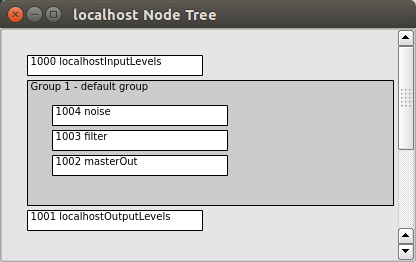
\includegraphics[scale=0.5]{fig-node-tree.png}}
\caption{A janela Node Tree}
\label{fig:node-tree}
\end{figure}

Os nódulos de Synth na janela Node Tree rodam de \emph{cima pra baixo}. Os synths mais recentes são adicionados no topo da pilha. Na figura \ref{fig:node-tree}, você pode ver que \texttt{"noise"} está no topo, \texttt{"filter"} vem em segundo, e \texttt{"masterOut"} aparece por último. Esta é a ordem correta que nós queremos para este exemplo: lendo de cima para baixo, o ruído branco passa para o filtro, e o resultado do filtro passa para o canal master. Tente agora rodar o exemplo de novo, mas de trás pra frente (ou seja, rode as linhas na ordem \texttt{n}, \texttt{f}, and \texttt{m}. Você não vai ouvir nada, porque os sinais estão sendo calculados na ordem errada.

Rodar as linhas certas na ordem certa é um método adequado em muitos casos, mas pode ser que isso fique um pouco complicado de controlar conforme o seu código vá ficando mais complexo. Para simplificar a tarefa, o SuperCollider permite que você defina explicitamente onde colocar os synths na janela Node Tree. Para tanto, usamos os argumentos \texttt{target} e \texttt{addAction}.

\begin{lstlisting}[style=SuperCollider-IDE, basicstyle=\scttfamily\footnotesize]
n = Synth("noise", addAction: 'addToHead');
m = Synth("masterOut", addAction: 'addToTail');
f = Synth("filter", target: n, addAction: 'addAfter');
\end{lstlisting}

Agora, não importa em que ordem você rodar as linhas acima, você pode ter certeza que os nódulos de cada synth vão ser colocados no lugar certo. O synth \texttt{"noise"} está sendo explicitamente adicionado na cabeça (topo) da janela Node Tree; o \texttt{"masterOut"} é adicionado na cauda (embaixo de todos os outros); e o \texttt{filter} é explicitamente adicionado logo depois do \texttt{n} (o synth de ruído).

\subsection{Grupos}

Conforme você começar a usar um monte de synths---alguns como fontes sonoras, outros para processamento, efeitos, seja lá o que você precisar---,pode ser uma boa ideia organizá-los em grupos. Aqui está um exemplo simples:

\begin{lstlisting}[style=SuperCollider-IDE, basicstyle=\scttfamily\footnotesize]
// Vá olhando tudo o que acontece na janela NodeTree
s.plotTree;

// Crie alguns canais de áudio
~reverbBus = Bus.audio(s, 2);
~masterBus = Bus.audio(s, 2);

// Defina os grupos
(
~sources = Group.new;
~effects = Group.new(~sources, \addAfter);
~master = Group.new(~effects, \addAfter);
)

// Rode todos os synths de uma vez
(
// Uma fonte de som qualquer
{
  Out.ar(~reverbBus, SinOsc.ar([800, 890])*LFPulse.ar(2)*0.1)
}.play(target: ~sources);

// Uma outra fonte sonora qualquer
{
  Out.ar(~reverbBus, WhiteNoise.ar(LFPulse.ar(2, 1/2, width: 0.05)*0.1))
}.play(target: ~sources);

// Uma pitada de reverb
{
  Out.ar(~masterBus, FreeVerb.ar(In.ar(~reverbBus, 2), mix: 0.5, room: 0.9))
}.play(target: ~effects);

// Um controle de volume com o mouse só porque é legal
{
  Out.ar(0, In.ar(~masterBus, 2) * MouseY.kr(0, 1))
}.play(target: ~master);
)
\end{lstlisting}

Para mais informações sobre ordem de execução, consulte os arquivos de ajuda ``Synth,'' ``Order of Execution,'' e ``Group.''
% PART V
\newpage
\part{E AGORA?}
Se você leu e mais ou menos entendeu tudo neste tutorial até agora, você já não é mais um iniciante em SuperCollider! Cobrimos um monte de material, e daqui pra frente você tem todas as ferramentas básicas necessárias para começar a desenvolver seus projetos pessoais, e continuar a aprender mais por conta própria. As seções a seguir fornecem uma breve introdução a alguns tópicos comuns de dificuldade intermediária. A última seção oferece uma lista concisa de outros tutoriais e fontes de aprendizado.

\section{MIDI}

Uma apresentação aprofundada dos conceitos e truques de MIDI está além do escopo deste tutorial. Os exemplos abaixo assumem alguma familiaridade com dispositivos MIDI e são fornecidos apenas como uma introdução.


\begin{lstlisting}[style=SuperCollider-IDE, basicstyle=\scttfamily\footnotesize]
// Jeito rápido de conectar todos os dispositivos disponíveis ao SC
MIDIIn.connectAll;

// Jeito rápido de ver todas as mensagens MIDI que estão chegando
MIDIFunc.trace(true);
MIDIFunc.trace(false); // pare de rastrear

// Jeito rápido de inspecionar todas as entradas CC
MIDIdef.cc(\someCC, {arg a, b; [a, b].postln});

// Obter entrada somente do cc 7, canal 0
MIDIdef.cc(\algumControleEspecifico, {arg a, b; [a, b].postln}, ccNum: 7, chan: 0);

// Uma SynthDef para testes rápidos
SynthDef("rápido", {arg freq, amp; Out.ar(0, SinOsc.ar(freq) * Env.perc(level: amp).kr(2))}).add;

// Toque de um teclado ou pad de percussão
(
MIDIdef.noteOn(\algumTeclado, { arg vel, nota;
	Synth("rápido", [\freq, nota.midicps, \amp, vel.linlin(0, 127, 0, 1)]);
});
)

// Criar um Pattern e o inicie pelo teclado
(
a = Pbind(
	\instrument, "rápido",
	\degree, Pwhite(0, 10, 5),
	\amp, Pwhite(0.05, 0.2),
	\dur, 0.1
);
)

// teste
a.play;

// Disparar o Pattern de um pad ou teclado
MIDIdef.noteOn(\algumTeclado, {arg vel, note; a.play});
\end{lstlisting}

Uma dúvida frequente é como administrar mensagens de "nota ligada" e "nota desligada" ("note on" e "note off") para notas sustentadas. Em outras palavras, quando você utiliza um envelope ADSR, você quer que cada nota seja sustentada enquanto a tecla estiver pressionada. O estágio de repouso ("release") inicia apenas quando o dedo solta a tecla correspondente (revise a seção sobre envelopes ADSR se necessário).

Para fazer isso, o SuperCollider simplesmente precisa monitorar qual nó de sintetizador corresponde a cada tecla. Podemos usar uma array para este fim, como demonstrado no exemplo abaixo. 

\begin{lstlisting}[style=SuperCollider-IDE, basicstyle=\scttfamily\footnotesize]
 // Uma SynthDef com envelope ADSR
SynthDef("rápido2", {arg freq = 440, amp = 0.1, gate = 1;
	var snd, env;
	env = Env.adsr(0.01, 0.1, 0.3, 2, amp).kr(2, gate);
	snd = Saw.ar([freq, freq*1.5], env);	
	Out.ar(0, snd)
}).add;

// Toque com um teclado MIDI

(
var arrayDeNotas = Array.newClear(128); // array com uma posição para cada nota MIDI possível

MIDIdef.noteOn(\minhaTeclaApertada, {arg vel, nota;
	arrayDeNotas[nota] = Synth("rápido2", [\freq, nota.midicps, \amp, vel.linlin(0, 127, 0, 1)]);
	["NOTA LIGADA", nota].postln;
});
	
MIDIdef.noteOff(\minhaTeclaLiberada, {arg vel, nota;
	arrayDeNotas[nota].set(\gate, 0);
	["NOTA DESLIGADA", nota].postln;
});
)
// PS. Garanta que as conexões MIDI do SC estejam ativas (MIDIIn.connectAll)
 \end{lstlisting} 
 
Para ajudar a entender o código acima:

\begin{itemize}
\item A SynthDef \texttt{"rápido2"} usa um envelope ADSR. O argumento \texttt{gate} é responsável por ligar e desligar as notas.
\item Um Array chamado \texttt{"arrayDeNotas"} é criado para monitorar quais notas estão sendo tocadas. Os índices do array devem corresponder aos números das notas MIDI sendo tocadas.
\item Toda vez que uma tecla é pressionada no teclado, um Synth começa a tocar (um nó de sintetizador é criado no servidor) e \emph{a referência a este nó de sintetizador é armazenada em uma posição exclusiva na array}; o índice da array é simplesmente o próprio número de nota MIDI.
\item Sempre que a tecla é liberada, a mensagem \texttt{.set(\textbackslash gate, 0)} é enviada para o nó de sintetizador apropriado, recuperado da array através do número da nota.
\end{itemize}

Nesta curta demonstração de MIDI apenas discutimos como enviar informação MIDI \emph{para} o SuperCollider. Para enviar mensagens MIDI \emph{a partir} do SuperCollider para algum outro programa ou equipamento MIDI, dê uma olhada no arquivo de Ajuda de \texttt{MIDIOut}.

\section{OSC}

OSC (Open Sound Control ou "Controle de Som Aberto") é uma excelente maneira de comunicar qualquer tipo de mensagem entre diferentes programas ou diferentes computadores em uma rede. Em muitos caos, é uma alternativa muito mais flexível às mensagens MIDI. Não temos espaço para explicar isso em mais detalhes aqui, mas o exemplo abaixo deve servir como um bom ponto de partida.

O objetivo desta demonstração é mandar mensagens OSC de um smartphone para seu computador ou de um computador para outro computador.

No computador receptor, rode este fragmento simples de código:

\bigskip
\begin{lstlisting}[style=SuperCollider-IDE, basicstyle=\scttfamily\footnotesize]
(
OSCdef(
	key: \seiLa,
	func: {arg ...args; args.postln},
	path: '/coisas')
)
\end{lstlisting}

Nota: pressionando [ctrl+.] interromperá o \texttt{OSCdef} e você não receberá mais mensagens.

\subsection{Mandando OSC para um outro computador}

Isso assume que ambos os computadores estejam rodando o SuperCollider e conectados a uma rede. Descubra o endereço IP do computador receptor e rode as seguintes linhas no computador emissor:

\begin{lstlisting}[style=SuperCollider-IDE, basicstyle=\scttfamily\footnotesize]
// Use isso na máquina que está mandando mensagens
~destino = NetAddr("127.0.0.1", 57120); // use o endereço IP correto para o computador de destino

~destino.sendMsg("/coisas", "aaloooo");
\end{lstlisting}

\subsection{Mandando OSC de um smartphone}

\begin{itemize}
\item Instale qualquer aplicativo grátis de OSC no telefone (por exemplo, gyrosc);
\item Entre o endereço IP do computador receptor no aplicativo OSC (como ‘target’);
\item Entre a porta de entrada do SuperCollider no app OSC (geralmente 57120);
\item Verifique o caminho de mensagem ("message path") que o aplicativo usa para mandar OSC e mude o seu OSCdef de acordo;
\item Tenha certeza que seu telefone está conectado à rede
\end{itemize}

Desde que seu telefone esteja enviando mensagens para o caminho correto, você deve vê-las chegando no computador.

\section{Quarks and plug-ins}

You can extended the functionality of SuperCollider by adding classes and UGens created by other users. \emph{Quarks} are packages of SuperCollider classes, extending what you can do in the SuperCollider language. \emph{UGen plugins} are extensions for the SuperCollider audio synthesis server.

Please visit \url{http://supercollider.github.io/} to get up-to-date information on how to add plug-ins and quarks to your SuperCollider installation. The ``Using Quarks'' Help file is also a good starting point: \url{http://doc.sccode.org/Guides/UsingQuarks.html}. From any SuperCollider document, you can evaluate \texttt{Quarks.gui} to see a list of all available quarks (it opens in a new window).

\section{Extra Resources}

This is the end of this introduction to SuperCollider. A few extra learning resources are listed below. Enjoy!

\begin{itemize}
\item An excellent series of YouTube tutorials by Eli Fieldsteel: \url{http://www.youtube.com/playlist?list=PLPYzvS8A_rTaNDweXe6PX4CXSGq4iEWYC}. 

\item The standard SC get-started tutorial by Scott Wilson and James Harkins, available online and in the built-in Help files: \url{http://doc.sccode.org/Tutorials/Getting-Started/00-Getting-Started-With-SC.html}

\item Nick Collins' online tutorial: \url{http://composerprogrammer.com/teaching/supercollider/sctutorial/tutorial.html}
 
\item The official SuperCollider mailing list is the best way to get friendly help from a large pool of users. Beginners are very welcome to ask questions in this list. You can sign up here: \url{http://www.birmingham.ac.uk/facilities/BEAST/research/supercollider/mailinglist.aspx}

\item Find a SuperCollider meet-up group in your city. The official sc-users mailing list is the best way to find out if there is one where you live. If there is no meet-up group in your area, start one!

\item Lots of interesting snippets of code can be found here: \url{http://sccode.org/}. Sign up for an account and share your code too.

\item Have you heard of SuperCollider tweets? \url{http://supercollider.github.io/community/sc140.html}

\end{itemize}


\newpage
% this adds the endnotes here
\theendnotes

% this ends the document
\end{document}
